\chapter{Estimaci\'on del fondo}
\label{ch:bkg}
% \epigraph{\emph{“Champions keep playing until they get it right.”}}{Billie Jean King}


Con la selección de eventos descripta en el \Ch{\ref{ch:evt_selection}}, los eventos con \acp{FP} y los eventos del canal \(t\) se redujeron en gran medida, aumenando la significancia de la señal, proporcionando as\'i un escenario excelente para la búsqueda de resonancias en el espectro de masas invariantes \myj. En este capítulo se describe en primer lugar (\Sect{\ref{sec:bkg:estimation}}) la estimación del fondo en estas regiones de señal, en particular aquel en el que un jet falsea un fotón. El fondo en este tipo de búsqueda de resonancia se modela con una función analítica, y se necesitan varios tests estadísticos para definirlo. En la \Sect{\ref{sec:bkg:modeling}}, se presenta la selección de la(s) función(es) óptima(s), donde se discuten en detalle todas los tests estadísticos para lograrlo.


\section{Estimación del fondo de jets falseando fotones}
\label{sec:bkg:estimation}

Los principales fondos encontrados para este análisis son aquellos en los que hay al menos un fotón y un jet en el estado final. Aunque los eventos \ac{SM} \gammajet (fotones prompt discutidos en \Sect{\ref{subsec:theory:sm:prompt_photon}}) son el fondo dominante, los eventos de jets falseando fotones son otra fuente importante de fondo que hay que tener en cuenta.




Los jets pueden ser identificados erróneamente como fotones (fotones falsos) si contienen un \pizero muy energético, dando lugar a un objeto \ac{EM} indistinguible de un fotón real y altamente energético (también llamado fotón prompt). Para hacer frente a los grandes fondos conteniendo jets se aplica el criterio de identificación \texttt{Tight} a los candidatos a fotón. Se espera que esta selección contenga fotones prompt con una contaminación de jet moderada. Como no se espera que esta tasa de identificación errónea se modele con precisión en \ac{MC}, se ha utilizado un método basado en datos. La identificación offline \texttt{Tight} es por diseño más ajustada que el trigger de fotones usado para recolectar los datos, por lo que hay una fracción no despreciable de jets candidatos a fotones que fallan el \ac{WP} \texttt{Tight} pero satisfacen alguna selección intermedia. Estos jets similares a fotones, a partir de ahora llamados pseudofotones (o \texttt{Non-Tight}), se definen como aquellos que pasan la identificación \texttt{Loose} pero fallan (al menos) uno de los cortes en las siguientes \acp{SS} utilizadas en la identificación \texttt{Tight}~\cite{ATLAS-EGamma-Performance-2015-2017}: \wone, \fside, \deltae y \eratio.

Para estimar el número de jets falseando fotones en las regiones de señal del presente análisis se emplea una combinación de dos métodos. Utilizando el método ABCD con las diferentes distribuciones de aislamiento calorimétrico de fotones reales y falsos es posible estimar lo que se conocen como \acp{FaF} que permiten obtener el número de fotones falsos en las regiones de señal~\cite{ATLAS-SUSY-PhotonMetX-13TeV,ATLAS-SUSY-PhotonMetX-13TeV-NOTE,ATLAS-SUSY-PhotonJetMet-13TeV,ATLAS-SUSY-PhotonJetMet-13TeV-NOTE}. El segundo método permite contar correctamente el número de fotones reales y falsos en las regiones delimitadas por el método ABCD, haciendo uso de un procedimiento secuencial de ajustes a la distribución de aislamiento de fotones en datos y \ac{MC}.

\begin{table}[ht!]
    \centering
    \caption{Selección de eventos utilizada para los estudios de jets falseando fotones utilizando el método ABCD y ajustes a las variables de \etiso. En la \Eqn{\ref{eq:objects:egamma:iso:definitions}} se define la expresión  de \ptiso.}
    \begin{tabular}{ l  c }
        \toprule
                                & Selección \\
        \midrule
        Trigger                 & HLT\_g140\_loose \\
        \ngamma                 & \(\ge1\) \\
        \ptgam [GeV]            & \(>150\) \\
        \ptjet [GeV]            & \(> 60\) \\
        \njets                  & \(>0\) \\
        \nlep                   & \(0\) \\
        Aislamiento de trazas   & \(\ptiso < 0.05\) \\
        \(|\etagam|\)           & \(\abseta < 1.37\) o \(1.52 < \abseta < 2.37\) \\
        \myj [GeV]              & \(\myj > 500\) \\
        \bottomrule
    \end{tabular}
    \label{tab:bkg:estimation:selection}
\end{table}

Para este estudio se utilizan fotones identificados con el \ac{WP} \texttt{Loose} y no aislados. Una descripción completa de la selección de eventos utilizada se encuentra en la \Tab{\ref{tab:bkg:estimation:selection}}.
Es importante señalar que los fotones \texttt{Tight} y aislados utilizados en la búsqueda son sólo un subconjunto de los utilizados en este estudio de estimación del fondo. Al requerir que los fotones \texttt{Loose} no aislados pasen la selección mostrada en la \Tab{\ref{tab:bkg:estimation:selection}} y además pasen la identificación \texttt{Tight} y \(\etiso < 0 ~\gev\) (ver la \Eqn{\ref{eq:objects:egamma:iso:definitions}}), se recuperan los fotones \texttt{Tight} y aislados utilizados en la búsqueda.
Finalmente se lleva a cabo un procedimiento manual de eliminaciones de objetos superpuestos entre los fotones y los jets para eliminar el jet solapado con el fotón \texttt{Loose} si \(\dryj<0.4\).

Este método se lleva a cabo utilizando datos, pero, dado que el \textit{unblinding} de los datos completos del Run-2 no se realiza hasta la última etapa del análisis, sólo se utiliza el conjunto de datos de 2015+2016, ya que ya fue observado en un trabajo anterior de la colaboración \ac{ATLAS}~\cite{ATLAS-PhotonJetResonances-2016}.


\subsection{Método ABCD}
\label{subsec:bkg:estimation:abcd}

El método ABCD define una región de señal \(A\) y tres regiones de control: \(B\), \(C\) y \(D\).
Estas regiones se definen variando el estado de identificación entre \texttt{Tight} y \texttt{Non-Tight}, y también cambiando los requisitos de aislamiento calorimétrico (aislado y no aislado)~\cite{ATLAS-EXOTICS-Monophoton-2017}.
La definición completa de las regiones ABCD es la siguiente
\begin{itemize}
    \item Región \(A\): Fotones \texttt{Tight} y \(\etiso < 0~ \gev\),
    \item Región \(B\): Fotones \texttt{Tight} y \(\etiso > 8~ \gev\),
    \item Región \(C\): Fotones \texttt{Non-Tight} y \(\etiso < 0~ \gev\),
    \item Región \(D\): Fotones \texttt{Non-Tight} y \(\etiso > 8~ \gev\),
\end{itemize}
donde \etiso se definió en la \Eqn{\ref{eq:objects:egamma:iso:definitions}}. La \Fig{\ref{fig:bkg:estimation:abcd:diagram}} muestra las cuatro regiones diferentes resultantes.

\begin{figure}[ht!]
    \centering
    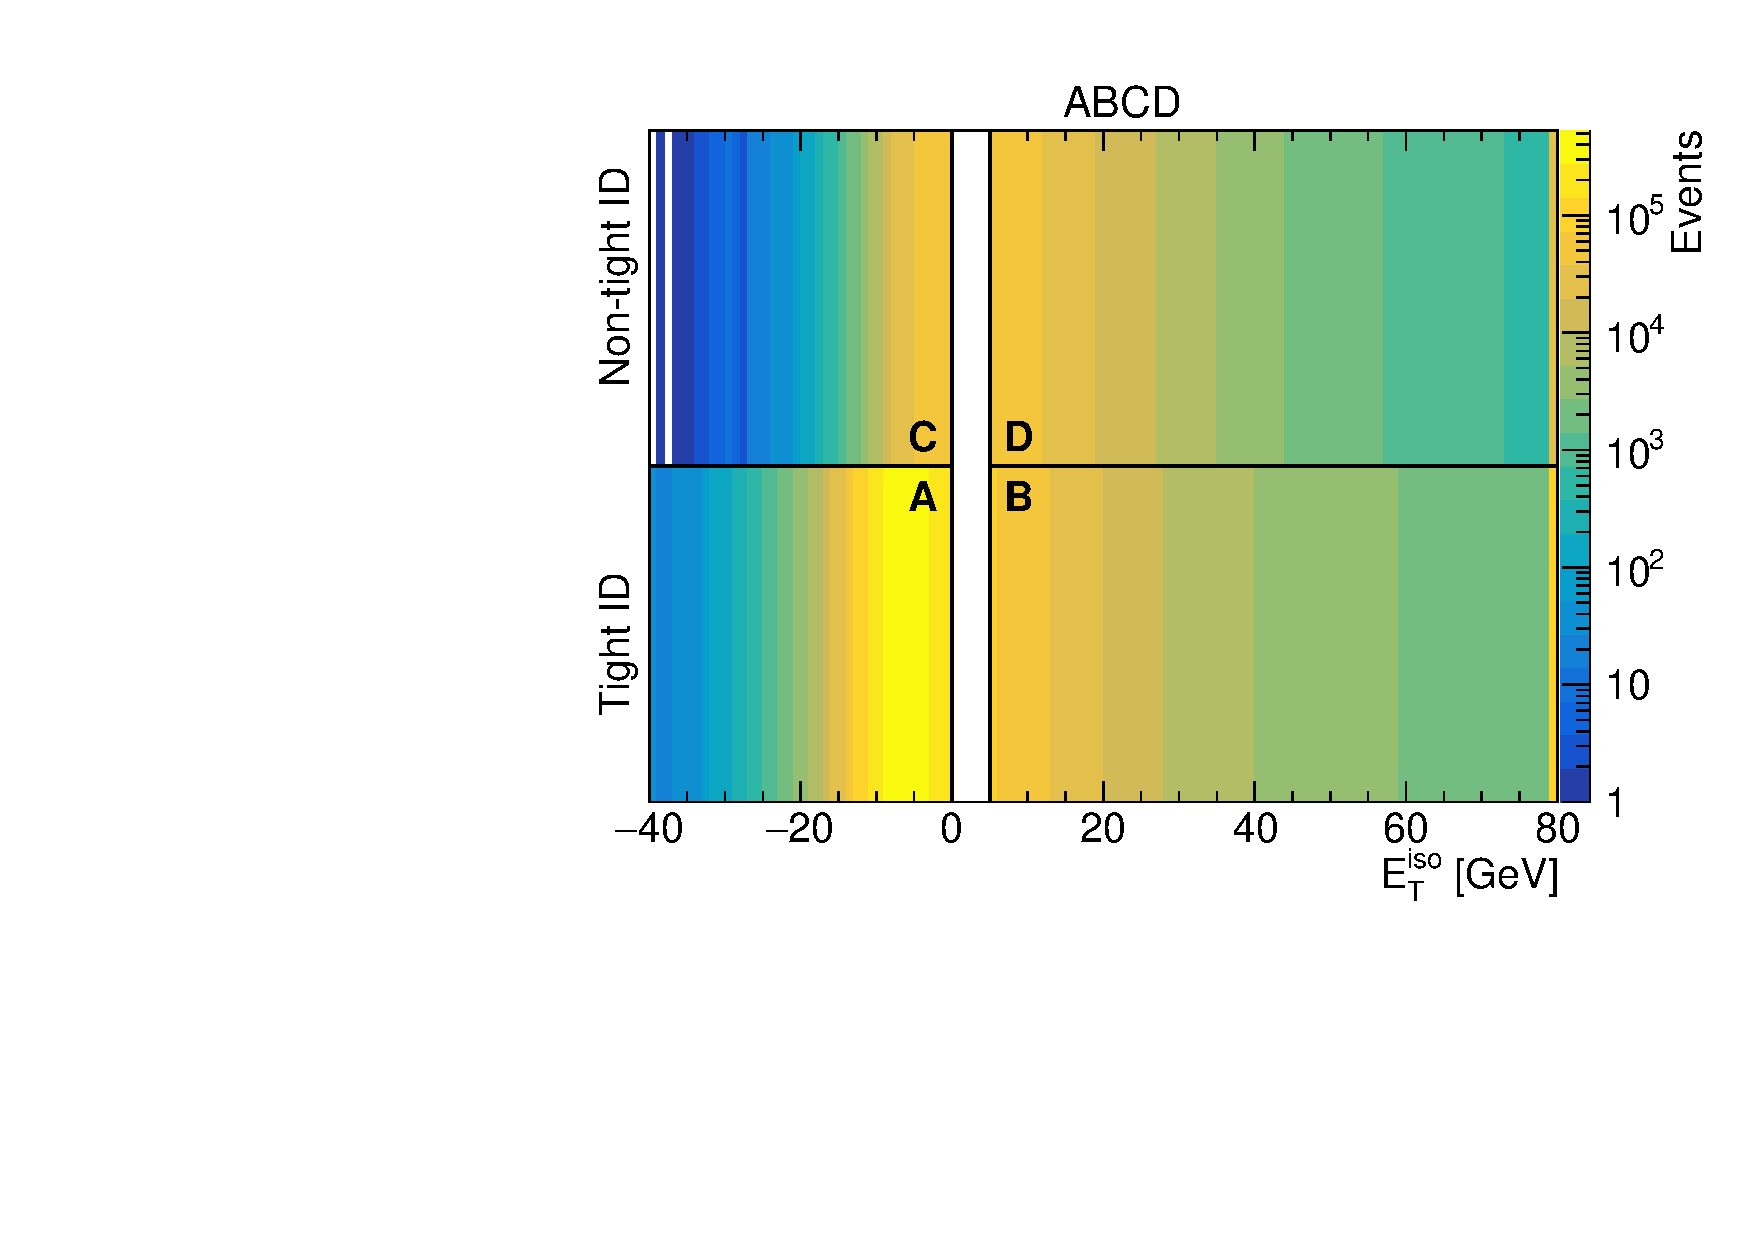
\includegraphics[width=0.65\textwidth]{5_resonances/bkg/estimation/ABCD_data_regions}
    \caption{Distribución bidimensional en el plano de identificación vs. \etiso obtenida de los datos.}
    \label{fig:bkg:estimation:abcd:diagram}
\end{figure}

Suponiendo que no hay contaminación de señal en ninguna región de control, las regiones \(B\), \(C\) y \(D\) sólo se componen de fondo \(N_{(B,C,D)}=N^{b}_{(B,C,D)}\). Además, suponiendo que no existe correlación entre el aislamiento y las \acp{SS} consideradas, se cumple la siguiente relación \(N^{b}_{B}/N^{b}_{A}=N^{b}_{D}/N^{b}_{C}\). Des esta forma, podrían definirse dos \acp{FaF} diferentes:
\begin{equation*}
    \ffiso = \frac{N_{C}}{N_{D}} \qquad \ffid = \frac{N_{B}}{N_{D}}
\end{equation*}
Por lo tanto, el número de jets que falsan fotones se puede estimar utilizando los \ac{FaF} como:
\begin{equation}
    \label{eq:bkg:estimation:abcd:njfakes}
    N_{\jfake} = N_{A} = \ffiso \times N_{B}  = \ffid \times N_{C}.
\end{equation}

Se podrían utilizar dos enfoques diferentes: modelar los fotones falsos utilizando fotones \texttt{Tight} pero no aislados de la región \(B\) utilizando los \ffiso, o modelar los fotones falsos utilizando el fotones \texttt{Non-Tight} pero aislados usando los \ffid.
Aunque ambos enfoques dan resultados equivalentes, se utiliza el enfoque \ffiso ya que conduce a estadísticas más altas.


Utilizando el \ac{FaF}, ahora es posible estimar la contribución de fondo de los jets falseando fotones en cada región del análisis (\(X\)). Para ello, se define una región de control de jets (CRJ-X) igual a la región \(X\) pero sustituyendo los requisitos de aislamiento por los utilizados en la región \(B\), y pesada por el correspondiente \ffiso:
\begin{equation*}
    N^{X}_{\jfake}(\pt) = \ffiso(\pt)\cdot N_{\text{CRJ-X}}(\pt)
\end{equation*}





\subsection{Correcciones al método de ABCD}
\label{subsec:bkg:estimation:abcd_corrections}

Deben aplicarse varias correcciones al método ABCD.
La primera consiste en considerar la posibilidad de una contaminación de señal en cualquiera de las regiones de control \(B\), \(C\) o \(D\) (fotones filtrados). Restando la cantidad de eventos de señal en estas regiones, la \Eqn{\ref{eq:bkg:estimation:abcd:njfakes}} se convierte en:
\begin{equation}
    \label{eq:bkg:estimation:abcd_corrections:njfakes_leak}
    N_{\jfake} = \frac{N_{B} - N_{B}^{s}}{N_{D} - N_{D}^{s}} \times (N_{C} - N_{C}^{s})
\end{equation}
donde \(N_{(B,C,D)}^{s}\) es el número de fotones reales en cada región. La estimación de estos números es una tarea complicada ya que se necesita para tener una descripción correcta de los fotones reales en los datos y está altamente contaminada con fotones falsos. El cálculo del número de fotones reales en los datos se realiza con un método de ajustes secuenciales a la distribución de aislamiento calorimétrico en los datos, que se explica con más detalle a continuación.


La presencia de una correlación residual del fondo en las cuatro regiones que puede manifestarse como una diferencia en las distribuciones del fondo para las regiones \texttt{Tight} y \texttt{Non-Tight} podría tenerse en cuenta calculando:
\begin{equation*}
    R = \frac{N^{b}_{A}\,N^{b}_{D}}{N^{b}_{B}\,N^{b}_{C}} \neq 1.
\end{equation*}
Sin embargo, como \(R\) no se puede encontrar en los datos porque eso significaría obtener \(N_A\) (es decir, mirar los datos en la región de se\~nal), se calcula un parámetro equivalente, que también se puede escribir utilizando teniendo en cuenta los fotones reales en las regiones de control:
\begin{equation*}
    R' = \frac{N_{A'}\,N_{D'}}{N_{B'}\,N_{C'}} = \frac{(N_{A'} - N^{s}_{A'})\,(N_{D'}-N^s_{D'})}{(N_{B'}-N^s_{B'})\,(N_{C'}-N^s_{C'})}
\end{equation*}
con la definición para cada región siendo:
\begin{itemize}
    \item región \(A'\): Fotones \texttt{Tight} y \(8 < \etiso < 15~ \gev\).
    \item región \(B'\): Fotones \texttt{Tight} y \(16 < \etiso < 80~ \gev\).
    \item región \(C'\): Fotones \texttt{Non-Tight} y \(8 < \etiso < 15~ \gev\).
    \item región \(D'\): Fotones \texttt{Non-Tight} y \(16 < \etiso < 80~ \gev\).
\end{itemize}
La selección particular de 8 \gev\ pretende definir una región sólo de fondo, pero manteniendo suficientes estadística para calcular los valores de \(R'\). En la \Fig{\ref{fig:bkg:estimation:abcd_corrections:rprime}} se muestran los valores \(R'\) en función de \ptgam.
Los valores están muy próximos a 1, con algunas excepciones en las que los valores se desvían de 1 en una cantidad máxima de \(\approx 20\%\) a bajo \ptgam.
\begin{figure}[htbp]
    \centering
    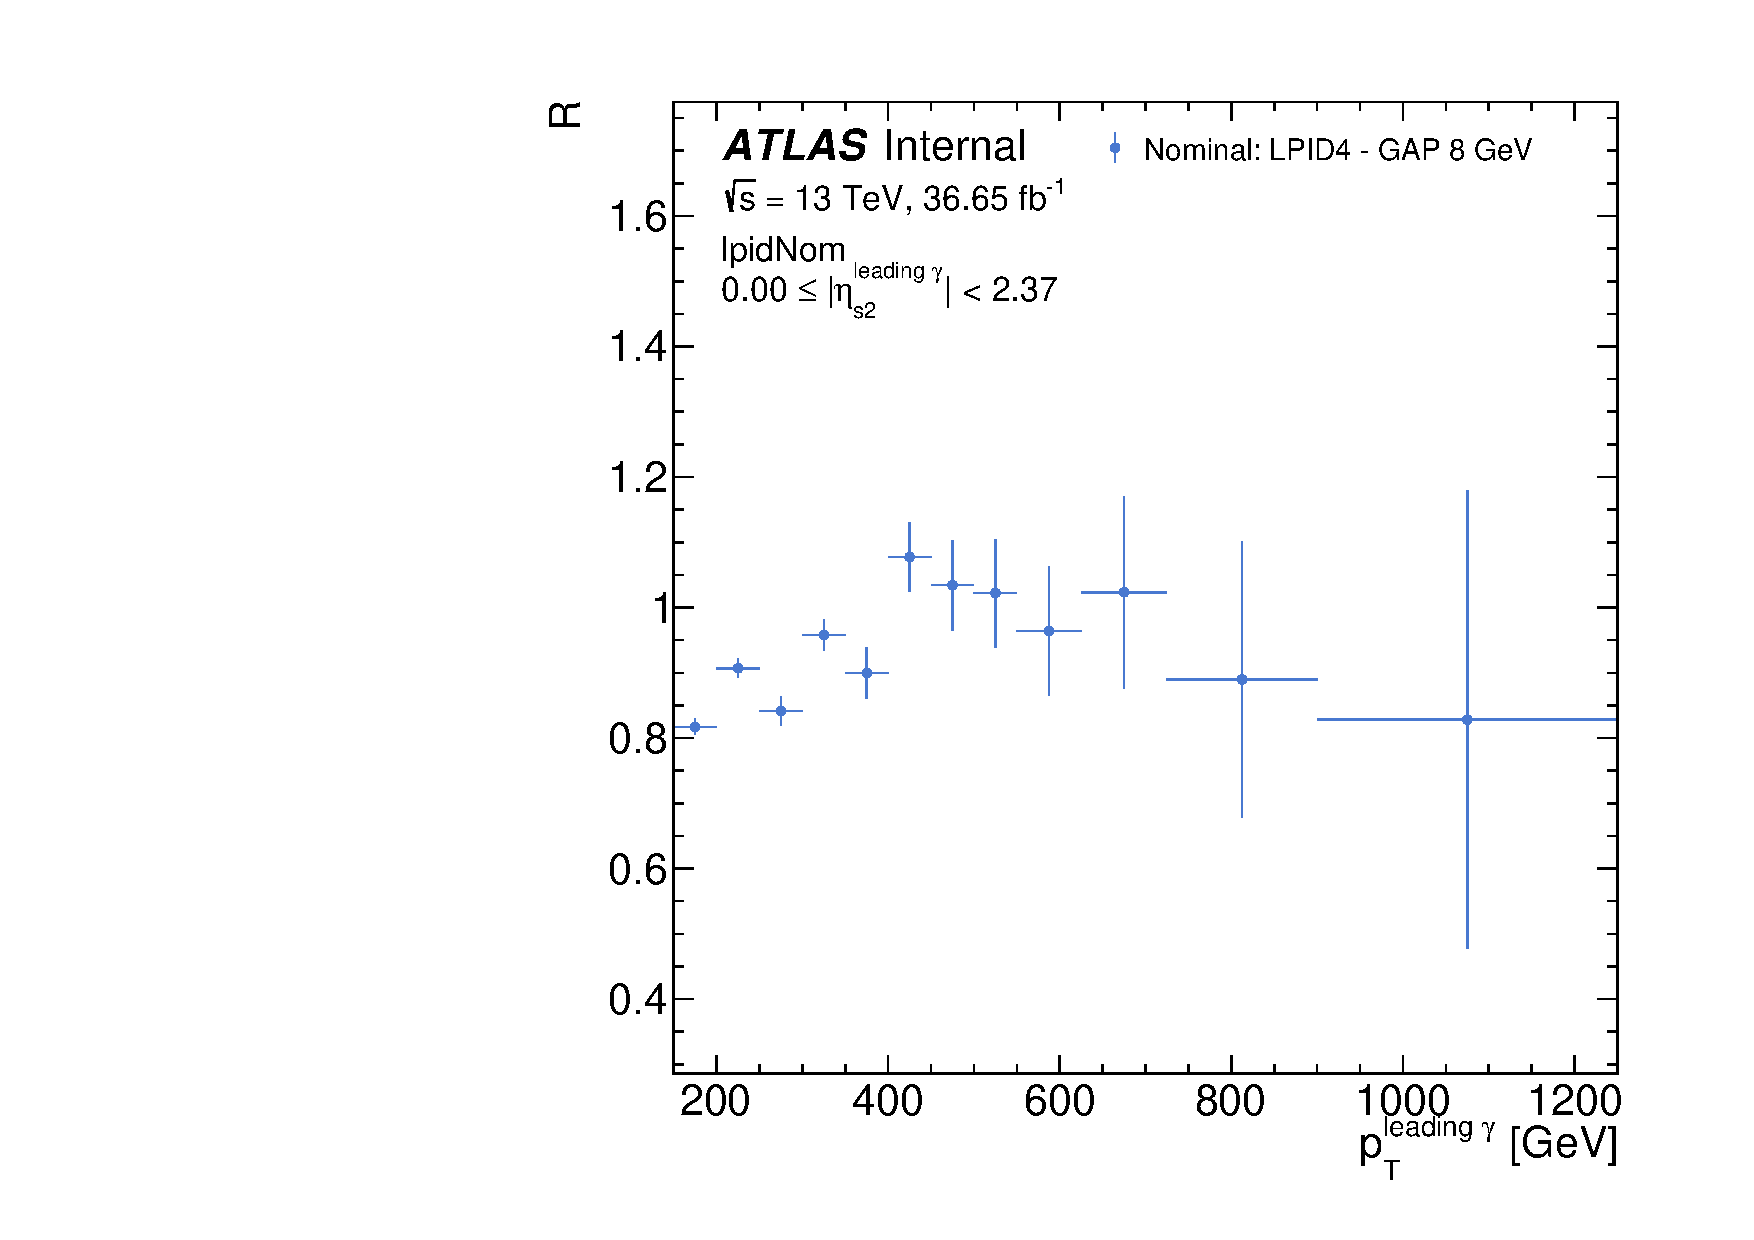
\includegraphics[width=0.5\linewidth]{5_resonances/bkg/estimation/coefficients/can__R__lpidNom__lph_pt0__abslph_etas20_0__2015_2016}
    \caption{Valores medidos de \(R'\) en función de \ptgam. Las barras de error muestran el error estadístico.}
    \label{fig:bkg:estimation:abcd_corrections:rprime}
\end{figure}

Por último, teniendo en cuenta los fotones filtrados en las regiones de control y las posibles correlaciones, la \Eqn{\ref{eq:bkg:estimation:abcd_corrections:njfakes_leak}} resulta, para el número esperado jets falseando fotones:
\begin{equation}
    \label{eq:bkg:estimation:abcd_corrections_ffiso}
    N_{\jfake}(\pt) =
    N^{b}_{A} =
    \left[R'  \frac{N_{C}-N^{s}_{C}}{N_{D}-N^{s}_{D}}  \left(1 - \frac{N^{s}_{B}}{N_{B}} \right)\right] \times N_B = \ffiso(\pt)  \times  N_{B}(\pt).
\end{equation}






\subsection{Procedimiento de ajustes al aislamiento calorimétrico}
\label{subsec:bkg:estimation:fits}


Para estimar el número de jets falseando fotones en las regiones de señal del análisis es necesario tener una estimación del número de eventos con fotones reales en las regiones de control del ABCD: regiones \(B\), \(C\) y \(D\). Para ello, se realiza una serie de ajustes a la distribución de aislamiento de los datos y de fotones reales obtenidos por \ac{MC}, tanto para fotones \texttt{Tight} como \texttt{Non-Tight}. El objetivo final de los ajustes secuenciales es contar con las componentes de fotones reales y falsos de los datos, que luego se utilizarán para calcular el número de fotones reales en las regiones de control ABCD. El procedimiento utiliza las muestras de \ac{MC} de las que se espera que únicamente contengan fotones reales. El cálculo se realiza en 11 bines de \ptgam:
\begin{equation*}
    \ptgam: \left[ 150, 200, 250, 300, 350, 400, 450, 500, 550, 625, 725, 900, \infty \right]~\gev.
\end{equation*}


La forma del aislamiento calorimétrico \etiso se ajusta de forma secuencial utilizando fotones que pasan los criterios de identificación \texttt{Tight} y \texttt{Non-Tight}, como se ha explicado anteriormente.
Por definición, los eventos con \(\etiso<0~\gev\) pasan el criterio de aislamiento calorimétrico y corresponden a fotones que caen en la región \(A\) si son \texttt{Tight} o \(C\) si son \texttt{Non-Tight}. Por otro lado, los eventos con \(\etiso>0~\gev\) definen las regiones \(B\) (fotones \texttt{Tight}) y \(D\) (fotones \texttt{Non-Tight}).
Tanto los fotones \texttt{Tight} como los \texttt{Non-Tight} contendrán un componente de fotones falsos que dominará sobre los fotones filtrados en el último caso~\cite{ATLAS-DiPhotonSearchIsolation-NOTE,ATLAS-EleMuPhoIsolation-NOTE}.

La secuencia de ajustes es la siguiente:
\begin{enumerate}
    \item \underline{Ajuste de fotones \texttt{Tight} en \ac{MC}}: Dado que las muestras de fotones prompt proporcionan una buena descripción de los fotones \texttt{Tight}, su distribución de \etiso se ajusta con una función \ac{CBall}\footnote{Esta función consiste en una función Gaussian pero una de las colas de ella está descripta por una forma funcional que sigue la ley de potencia.}. Se encontró que la simple descripción \ac{CBall} no se acomoda bien en toda el rango ajustado, especialmente en la zona del pico de la distribución de \etiso, por lo tanto se requiere de una función más flexible. De este modo, se utiliza una versión mejorada de la \ac{CBall}: la \ac{DSACB}\footnote{Como su nombre sugiere, en una \ac{DSACB}, las dos colas se modelan mediante funciones que siguen de ley de potencia, y el núcleo de la distribución gaussiana tiene dos desviaciones estándar diferentes, de ahí la asimetría.}.
    % Aunque la descripción es mucho mejor en este caso, el núcleo gaussiano sigue teniendo dificultades para modelar correctamente el pico de la distribución.
    \item \underline{Fotones filtrados}: La forma de los fotones falsos se estima sustrayendo la componente de fotones filtrados (obtenida de la simulación \ac{MC}) a los datos en todo el rango \etiso. Esto proporciona una descripción muy buena de la componente de fotones falsos en las regiones \texttt{Non-Tight} (eso es, regiones \(C\) y \(D\)).
    \item \underline{Ajuste combinado a los datos en regiones \texttt{Tight}}: Utilizando la forma de fotones reales brindada por la función \ac{DSACB} estimada en el primer paso y la forma de fotones falsos estimada en el paso anterior, se realiza un ajuste combinado a la distribución \etiso de fotones \texttt{Tight} de los datos. Ejemplos del ajuste resultante en tres bines de \pt se muestran en la \Fig{\ref{fig:bkg:estimation:fits_tightID_data}}.
    
        La distribución final concuerda bien con los datos, lo que indica la correcta selección de las distribuciones para cada componente. El componente de fotones reales es el responsable del pico en valores bajos de aislamiento, mientras que las componentes de fotones falsos contribuyen principalmente en el rango \(0~\gev < \etiso < 40 ~\gev\) contribuyendo al número total de eventos mucho menos que los reales como era de esperar. Pueden observarse algunas diferencias entre el ajuste combinado y los datos cerca del pico de la distribución, que es evidente en los residuos normalizados del ajuste. Esta diferencia también se observó en el primer paso del cálculo al modelar las componentes de los fotones reales y tiene su origen directo en el modelado gaussiano del pico.

        \begin{figure}[bth!]
            \centering
            \begin{subfigure}[h]{0.32\linewidth}
                \centering
                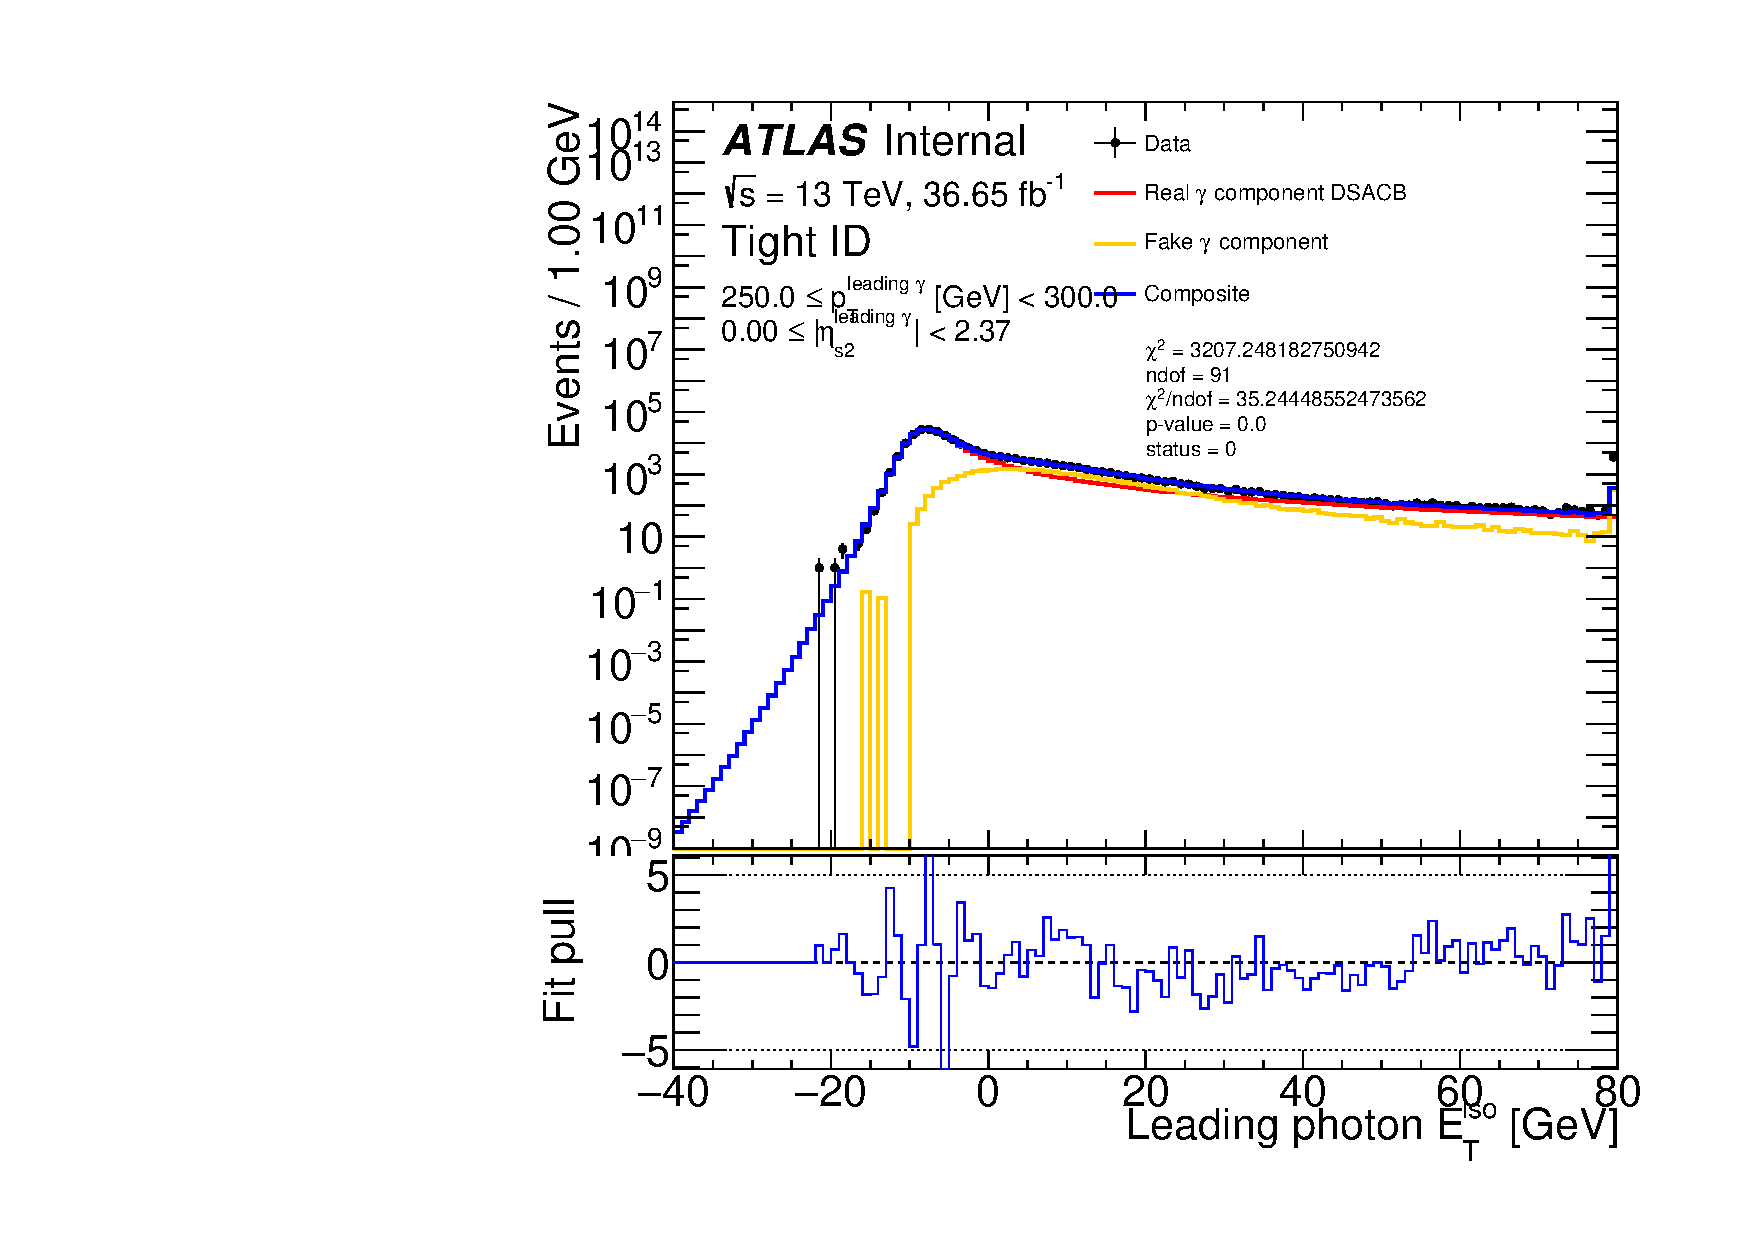
\includegraphics[width=\linewidth]{5_resonances/bkg/estimation/fits/lpid4/2015_2016/lph_pt0/lph_pt0__250p0/data__tight__composite__lph_pt0__250p0__abslph_etas20__0p00}
                \caption{\(250 < \ptgam < 300~\gev\).}
            \end{subfigure}
            \begin{subfigure}[h]{0.32\linewidth}
                \centering
                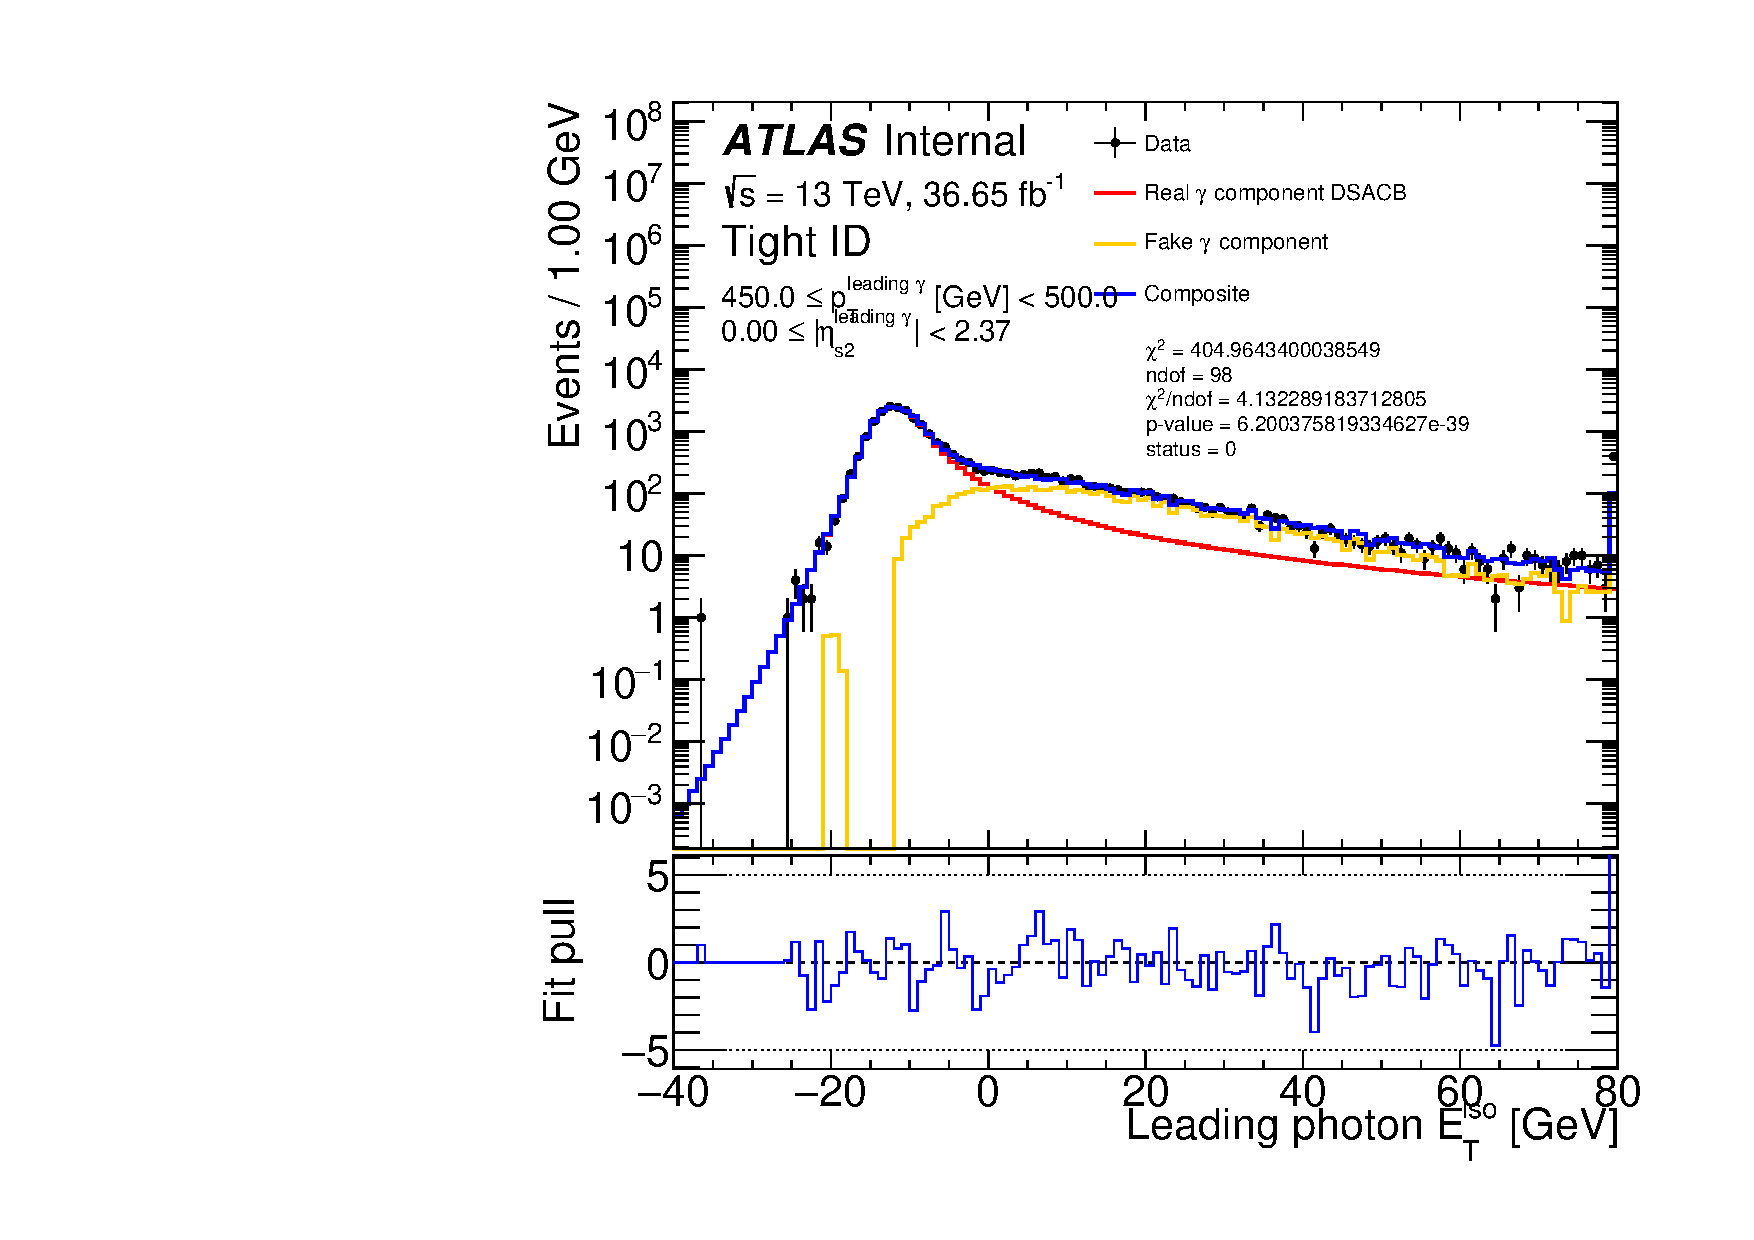
\includegraphics[width=\linewidth]{5_resonances/bkg/estimation/fits/lpid4/2015_2016/lph_pt0/lph_pt0__450p0/data__tight__composite__lph_pt0__450p0__abslph_etas20__0p00}
                \caption{\(450 < \ptgam < 500~\gev\).}
            \end{subfigure}
            \begin{subfigure}[h]{0.32\linewidth}
                \centering
                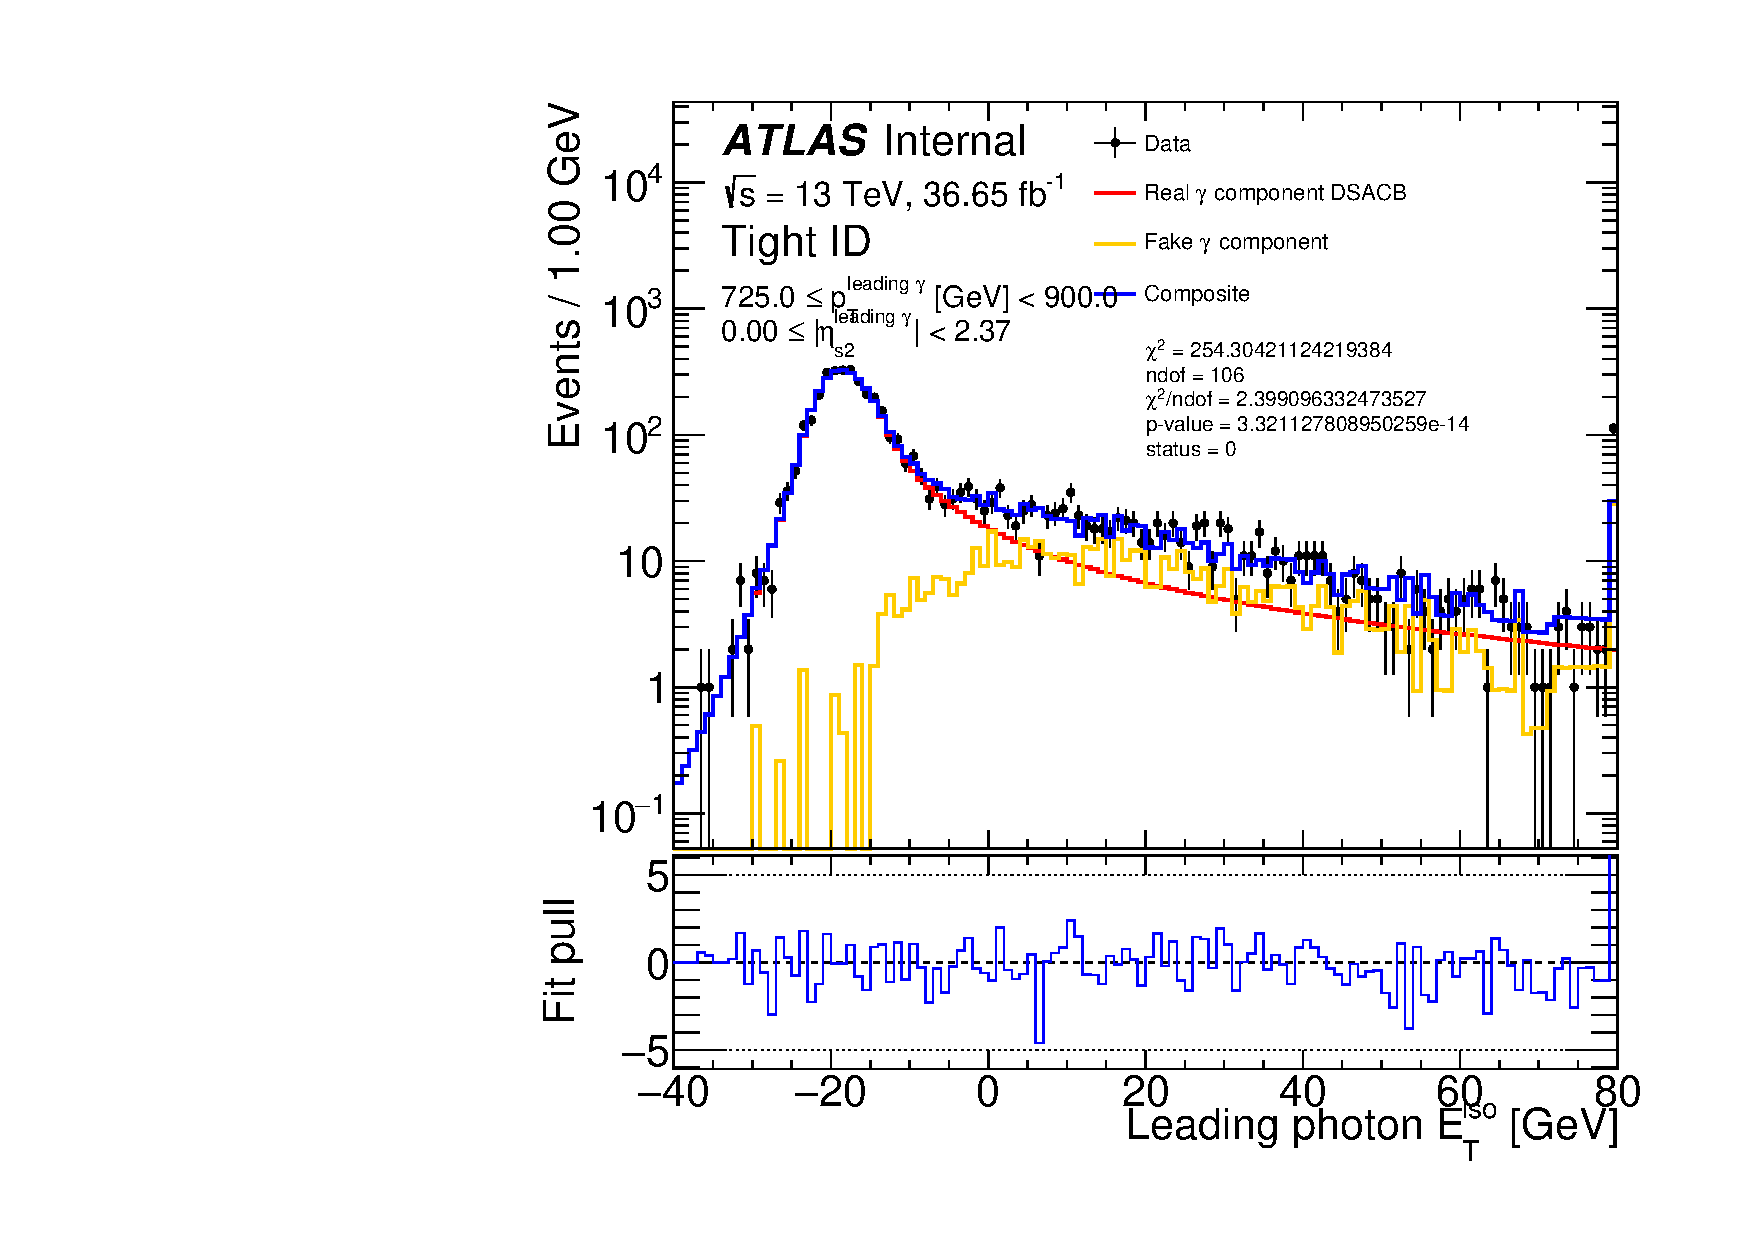
\includegraphics[width=\linewidth]{5_resonances/bkg/estimation/fits/lpid4/2015_2016/lph_pt0/lph_pt0__725p0/data__tight__composite__lph_pt0__725p0__abslph_etas20__0p00}
                \caption{\(725 < \ptgam < 900~\gev\).}
            \end{subfigure}
            \caption{Ajuste combinado a los datos. La curva roja representa la componente de fotones reales, que se representa mediante una función del tipo \ac{DSACB}, calculada en el primer paso de la secuencia de ajustes. El histograma amarillo es la contribución de los fotones falsos, obtenida en el segundo paso. El panel inferior de las figuras muestran los residuos normalizados (o pull) de los ajustes.}
            \label{fig:bkg:estimation:fits_tightID_data}
        \end{figure}
\end{enumerate}





\subsection{Resultados}
\label{subsec:bkg:estimation:results}

Del procedimiento anterior, que utiliza el método ABCD y una secuencia de ajustes usando la distribución de \etiso se pueden extraer varias cifras clave. En primer lugar, una variable importante para comprender mejor la física subyacente es la pureza de procesos \gammajet, calculada como
\[
    P_A = \frac{
        N^{A}_{\text{real}\gamma, \text{postfit}}
    }{
        N^{A}_{\text{real}\gamma, \text{postfit}} + N^{A}_{\text{fake}\gamma, \text{postfit}}
    }.
\]
Estas purezas se muestran en la \Fig{\ref{fig:bkg:estimation:results:results:purities}} y sus valores numéricos en la \Tab{\ref{tab:bkg:estimation:results:ffiso_purity_values}}. Como puede observarse, se alcanzan purezas mayores al \(92\%\) en todo el rango de \ptgam, lo que indica que los procesos que contienen un fotón real y un jet abarcan la mayor parte de la muestra, mientras que la fracción de los procesos de jet falseando fotones son menores al \(10\%\).
% Las medidas de pureza se suavizan utilizando un spline de orden \(3^{\text{rd}}\), mostrado con la línea roja en la figura.

\begin{table}[ht!]
    \caption{\acp{FaF} y purezas en función de \ptgam calculadas con los métodos descriptos previamente.}
    \begin{tabular}{lcc}
        \toprule
        \(p_{T}^{\text{leading} \gamma}\) [GeV] & \(FF_{\text{iso}}\) &  Pureza de \(\gamma\) reales en region \(A\) \\
        \midrule
        $150-200$    & $0.1873$ & $0.9201$ \\
        $200-250$    & $0.1885$ & $0.9321$ \\
        $250-300$    & $0.1901$ & $0.9418$ \\
        $300-350$    & $0.1918$ & $0.9494$ \\
        $350-400$    & $0.1934$ & $0.9552$ \\
        $400-450$    & $0.1948$ & $0.9593$ \\
        $450-500$    & $0.1956$ & $0.9620$ \\
        $500-550$    & $0.1956$ & $0.9636$ \\
        $550-625$    & $0.1943$ & $0.9642$ \\
        $625-725$    & $0.1891$ & $0.9633$ \\
        $725-900$    & $0.1703$ & $0.9604$ \\
        $900-\infty$ & $0.0835$ & $0.9650$ \\
        \bottomrule
    \end{tabular}
    \label{tab:bkg:estimation:results:ffiso_purity_values}
    \centering
\end{table}




\begin{figure}[ht!]
    \centering
    \begin{subfigure}[h]{0.49\linewidth}
        \centering
        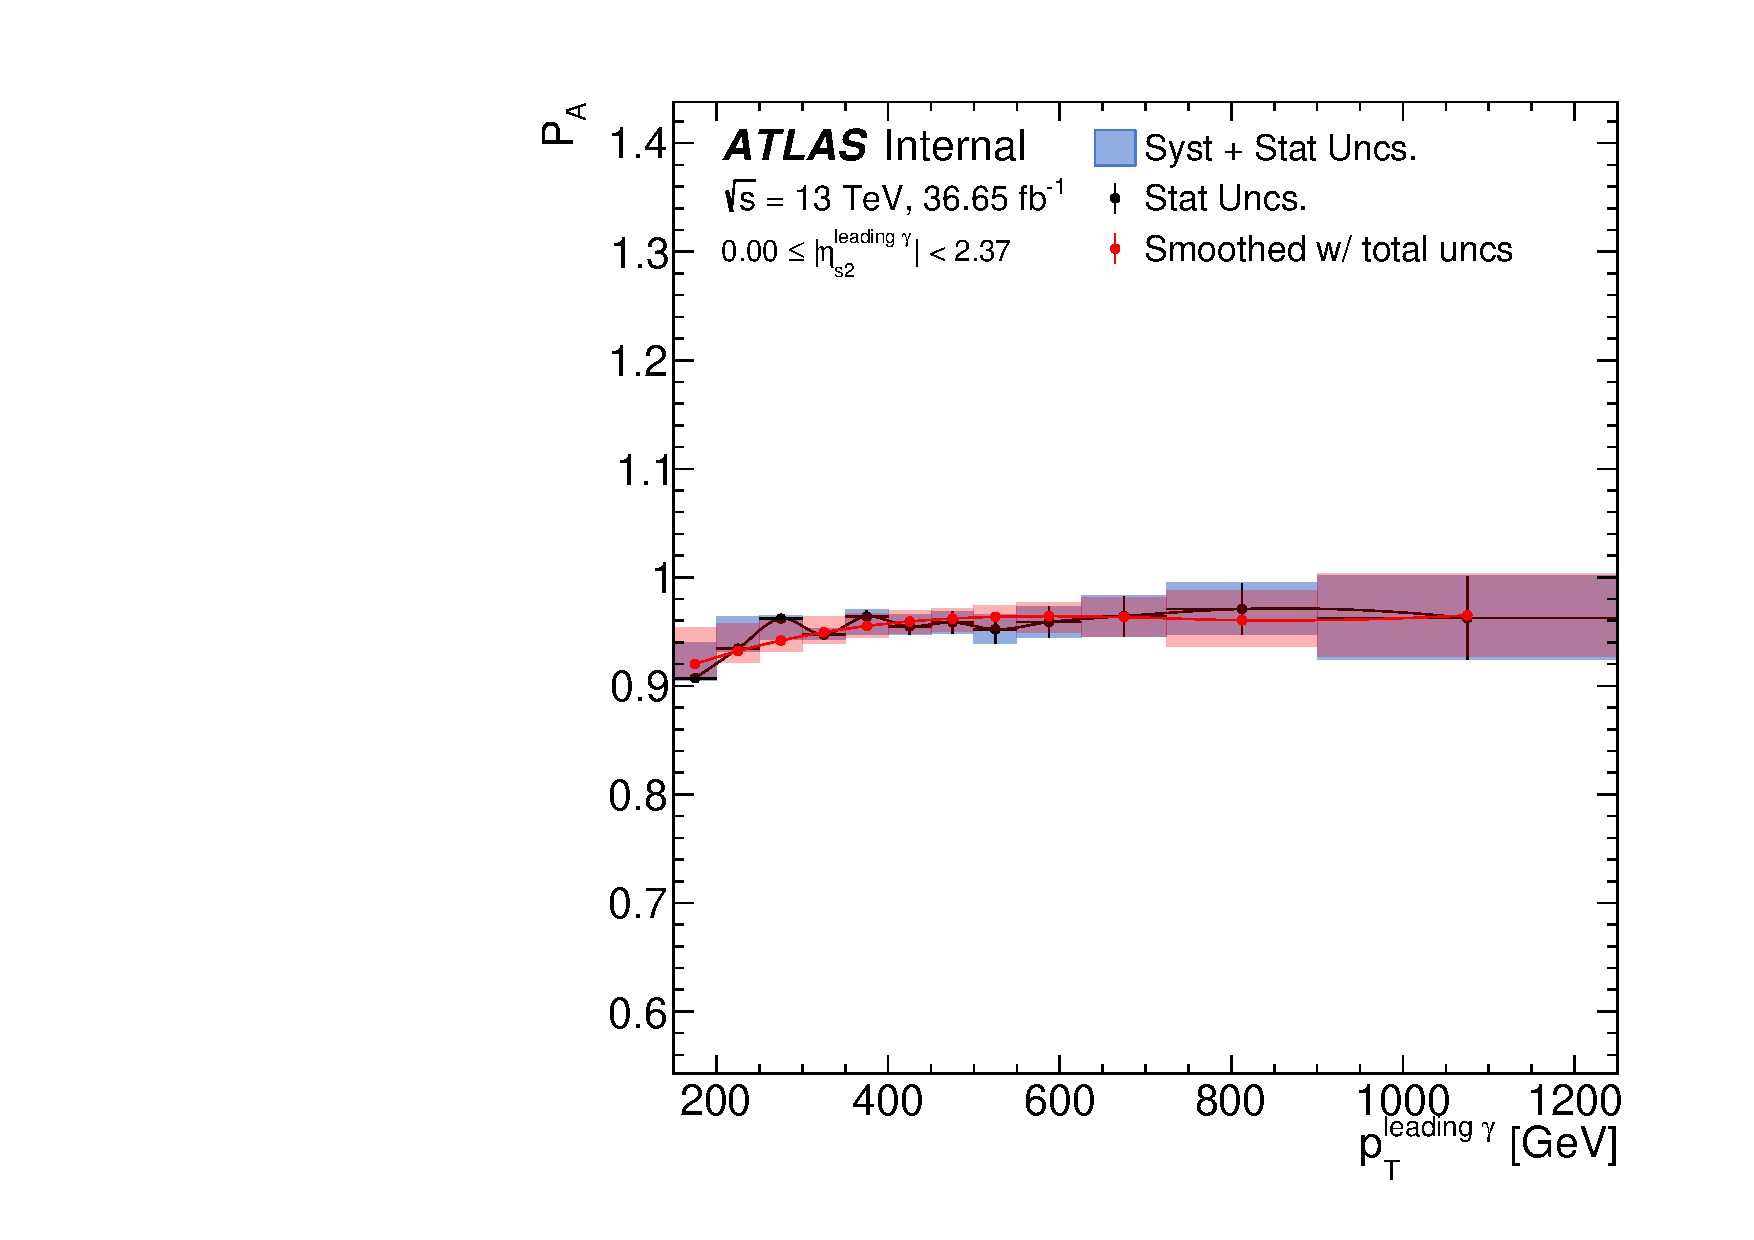
\includegraphics[width=\linewidth]{5_resonances/bkg/estimation/coefficients/can__purity_real_A__withsysts__lph_pt0__abslph_etas20_abslph_etas20__0p00__2015_2016}
        \caption{\(P_A\).}
        \label{fig:bkg:estimation:results:results:purities}
    \end{subfigure}
    \hfill
    \begin{subfigure}[h]{0.49\linewidth}
        \centering
        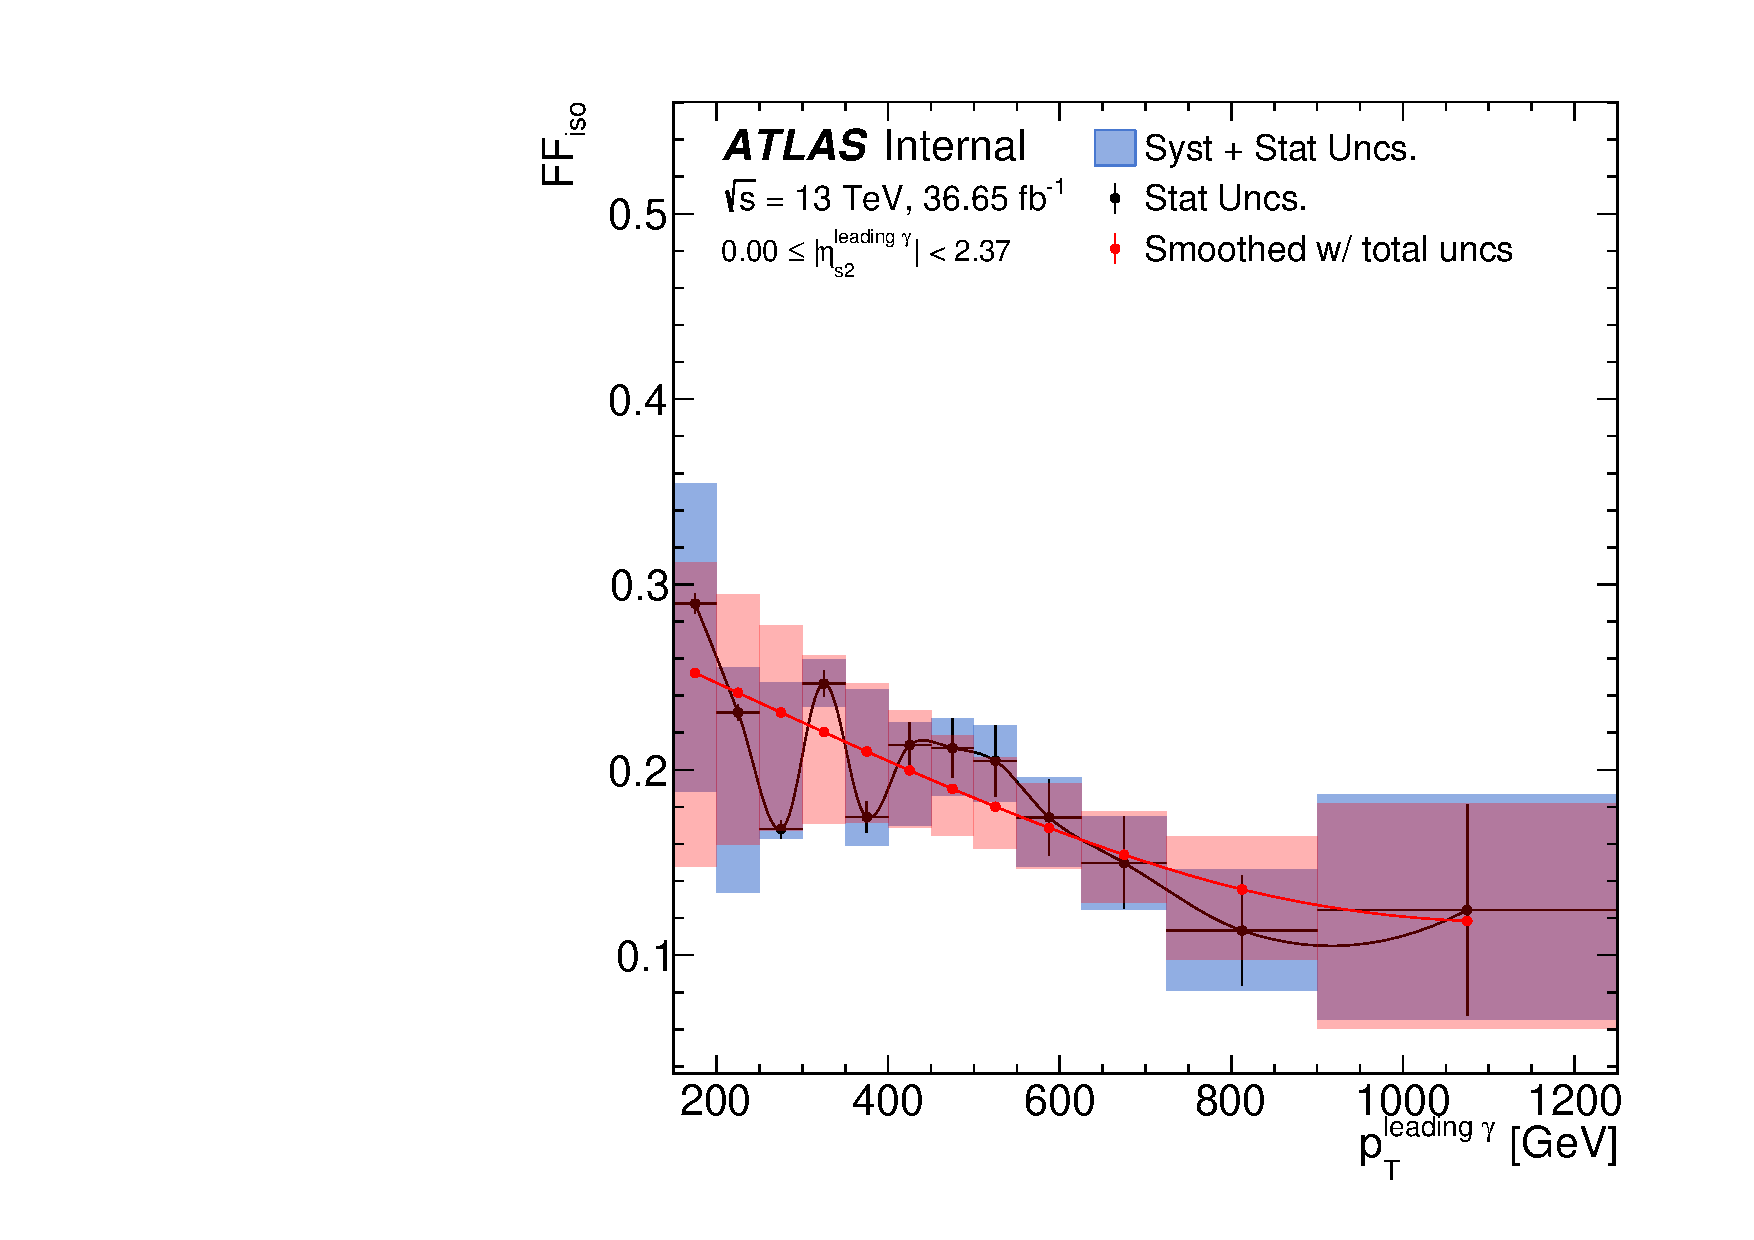
\includegraphics[width=\linewidth]{5_resonances/bkg/estimation/coefficients/can__FF_iso__withsysts__lph_pt0__abslph_etas20_abslph_etas20__0p00__2015_2016}
        \caption{\ffiso.}
        \label{fig:bkg:estimation:results:results:ffiso}
    \end{subfigure}
    \caption{Valores medidos de la pureza de \gammajet \(P_A\) (izquierda) y de los \ffiso (derecha) como función de \ptgam utilizando el método ABCD. Las medidas se muestran con los puntos negros (sólo con incerteza estadística), las áreas sombreadas de azul muestran la incerteza total (estadística y sistemática añadidas en cuadratura) y los puntos rojos con las áreas sombreadas rojas las medidas suavizadas utilizando una interpolación \textit{spline} de tercer orden.}
    \label{fig:bkg:estimation:results:results}
\end{figure}


Los \acp{FaF}, y en particular \ffiso, se aplican a los eventos de datos en una región de control CRJ-X, que sólo difiere de cualquier región de señal \(X\) en el análisis al requerir fotones no aislados. Los valores de \ffiso, por tanto, pueden interpretarse como la probabilidad de que un jet falsee un fotón en la región \(X\) dada la tasa de fotones falsos en CRJ-X. Los resultados se muestran con los puntos negros en la \Fig{\ref{fig:bkg:estimation:results:results:ffiso}} y las incertezas totales con las áreas sombreadas en azul. Como se desprende en estos resultados, se observan valores \ffiso inestables para \(\ptgam<400~\gev\) lo que puede llevar a bumps espurios introducidos por el propio método. Para ello, los valores fueron interpolados utilizando un método de \textit{spline} de tercer orden. Los valores numéricos de los \ffiso se muestran en la \Tab{\ref{tab:bkg:estimation:results:ffiso_purity_values}}.
\section{Modelado del fondo}
\label{sec:bkg:modeling}


La tarea más compleja en una búsqueda de resonancias es el correcto modelado del fondo. Como se ha mencionado anteriormente, este análisis sólo hace uso de las muestras simuladas del fondo para optimizar la selección de eventos y seleccionar las posibles formas funcionales para modelar el fondo. Al mismo tiempo que se selecciona la forma funcional óptima, se selecciona el rango en el que se realizarán los ajustes, para luego clasificar las combinaciones de modelos funcionales y rangos de ajuste basándose en el valor de la \acf{SSig}.
Una vez que se realiza la búsqueda propiamente dicha en los datos, se utiliza la función del fondo y el rango de ajuste que da la \ac{SSig} más baja para ajustar los datos, teniendo entonces un caso en el que el fondo es modelado por los datos.













\subsection{Familia de funciones}
\label{subsec:bkg:modeling:functions}

Para modelar los fondos irreducibles y reducibles de forma inclusiva, se utiliza la siguiente familia de funciones que presentan un decaimiento suave:
\begin{equation}
    \label{eq:bkg:modeling:functions:general_equation}
    f_{b}( x \equiv \myj / \sqrt{s}) = (1-x)^{p_0} x^{-\sum_{i=1} p_i \left(\ln x\right)^{i-1}} 
\end{equation}
Esta familia de funciones se usa habitualmente en búsquedas de resonancias en un espectro de fondo de decaimiento suave, como aquellos brindados por estados finales de dos jets, de pares fotón+jet~\cite{ATLAS-Dijet-2019,ATLAS-PhotonJetResonances-2016}. Estas, además, permiten modificar la forma funcional añadiendo o quitando \ac{dof}. Existen múltiples formas de añadir \acp{dof} adicionales, cada una de las cuales tiene un efecto diferente en el ajuste. La función de fondo siempre se escalará por su normalización, aunque en la \Eqn{\ref{eq:bkg:modeling:functions:general_equation}} se omite el parámetro. La función de fondo final es:
\begin{equation}
    \label{eq:bkg:modeling:functions:general_equation_normalization}
    f_{b}( x \equiv \myj / \sqrt{s}) = n_{\text{bkg}\, }(1-x)^{p_0} x^{-\sum_{i=1} p_i \left(\ln x\right)^{i-1}} 
\end{equation}
En lo que sigue, al contar el número de parámetros se incluye la normalización. Por ejemplo, una función \textit{dof3} tendrá 3 parámetros que controlan su forma y uno que controla la normalización, por lo que tendrá un total de 4 parámetros.

Estas funciones se prueban en predicciones \ac{MC}, con el fin de determinar qué funciones deben considerarse para el ajuste de las distribuciones de datos.
La elección se realiza teniendo en cuenta la estadística total del espectro de \myj, los tests de \acp{SSig}, tests de inyección de señal y tests \(F\).










\subsection{Preparación de las muestras}
\label{subsec:bkg:modeling:preparation}

Para los estudios de modelización del fondo se utilizan dos tipos diferentes de muestras: toys y Asimov. Estas muestras se derivan directamente de la distribución de fondo del \ac{MC}, que consiste en eventos de \gammajet y de jet falseando fotones. La estrategia para generar estas muestras se resume en el diagrama de la \Fig{\ref{fig:bkg:modeling:preparation:datasets_generation}} y a continuación se describe detalladamente cada paso.

\begin{figure}[ht!]
    \centering
    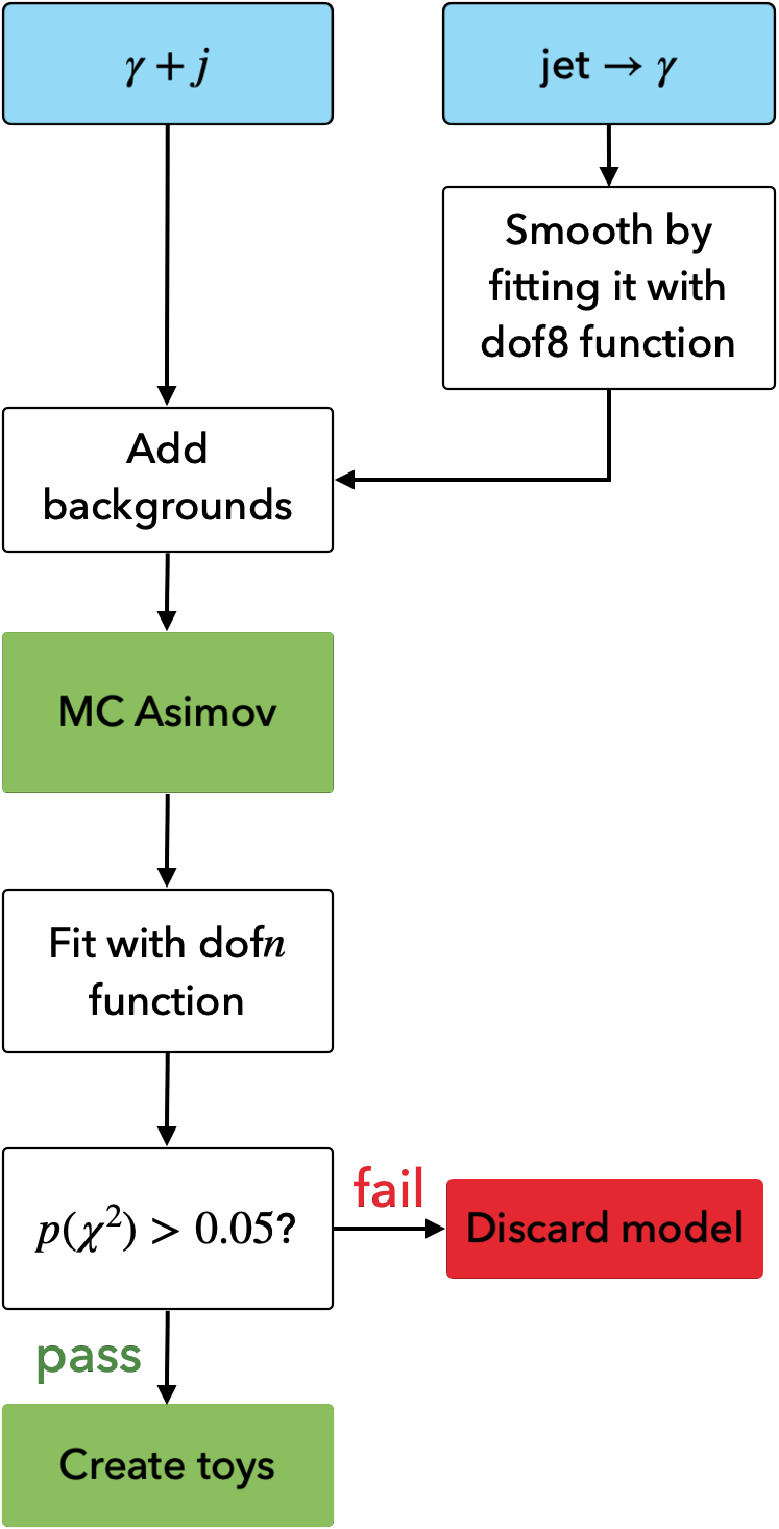
\includegraphics[width=0.3\linewidth]{5_resonances/bkg/modeling/toys_generation}
    \caption{Procedimiento para la preparación de las muestras del fondo para estimar la forma funcional.}
    \label{fig:bkg:modeling:preparation:datasets_generation}
\end{figure}




\subsubsection{Suavizado del fondo de jets falseando fotones}
\label{subsubsec:bkg:modeling:preparation:jfakes_smooth}


Se observó que aproximadamente \(5\%\) de la muestra \gammajet está poblada por eventos de fotones falsos. Este fondo se estima directamente a partir de datos en regiones de control que fallan el aislamiento calorimétrico, y luego se pesa por el \ac{FaF} correspondiente en función del \ptgam. Sin embargo, especialmente a valores altos de \myj, se encuentra que hay muy pocos eventos pero que cuando se añaden al fondo dominante de \gammajet, distorsionan la distribución suave y empiezan a aparecer bumps artificiales, mostrados en la \Fig{\ref{fig:bkg:modeling:preparation:jfakes_smooth:bkg_myj_distribution}}.
Además, cabe notar que la contribución de los fotones falsos es siempre un orden de magnitud menor que el fondo de \gammajet.

\begin{figure}[ht!]
    \centering
    \begin{subfigure}[h]{0.49\linewidth}
        \centering
        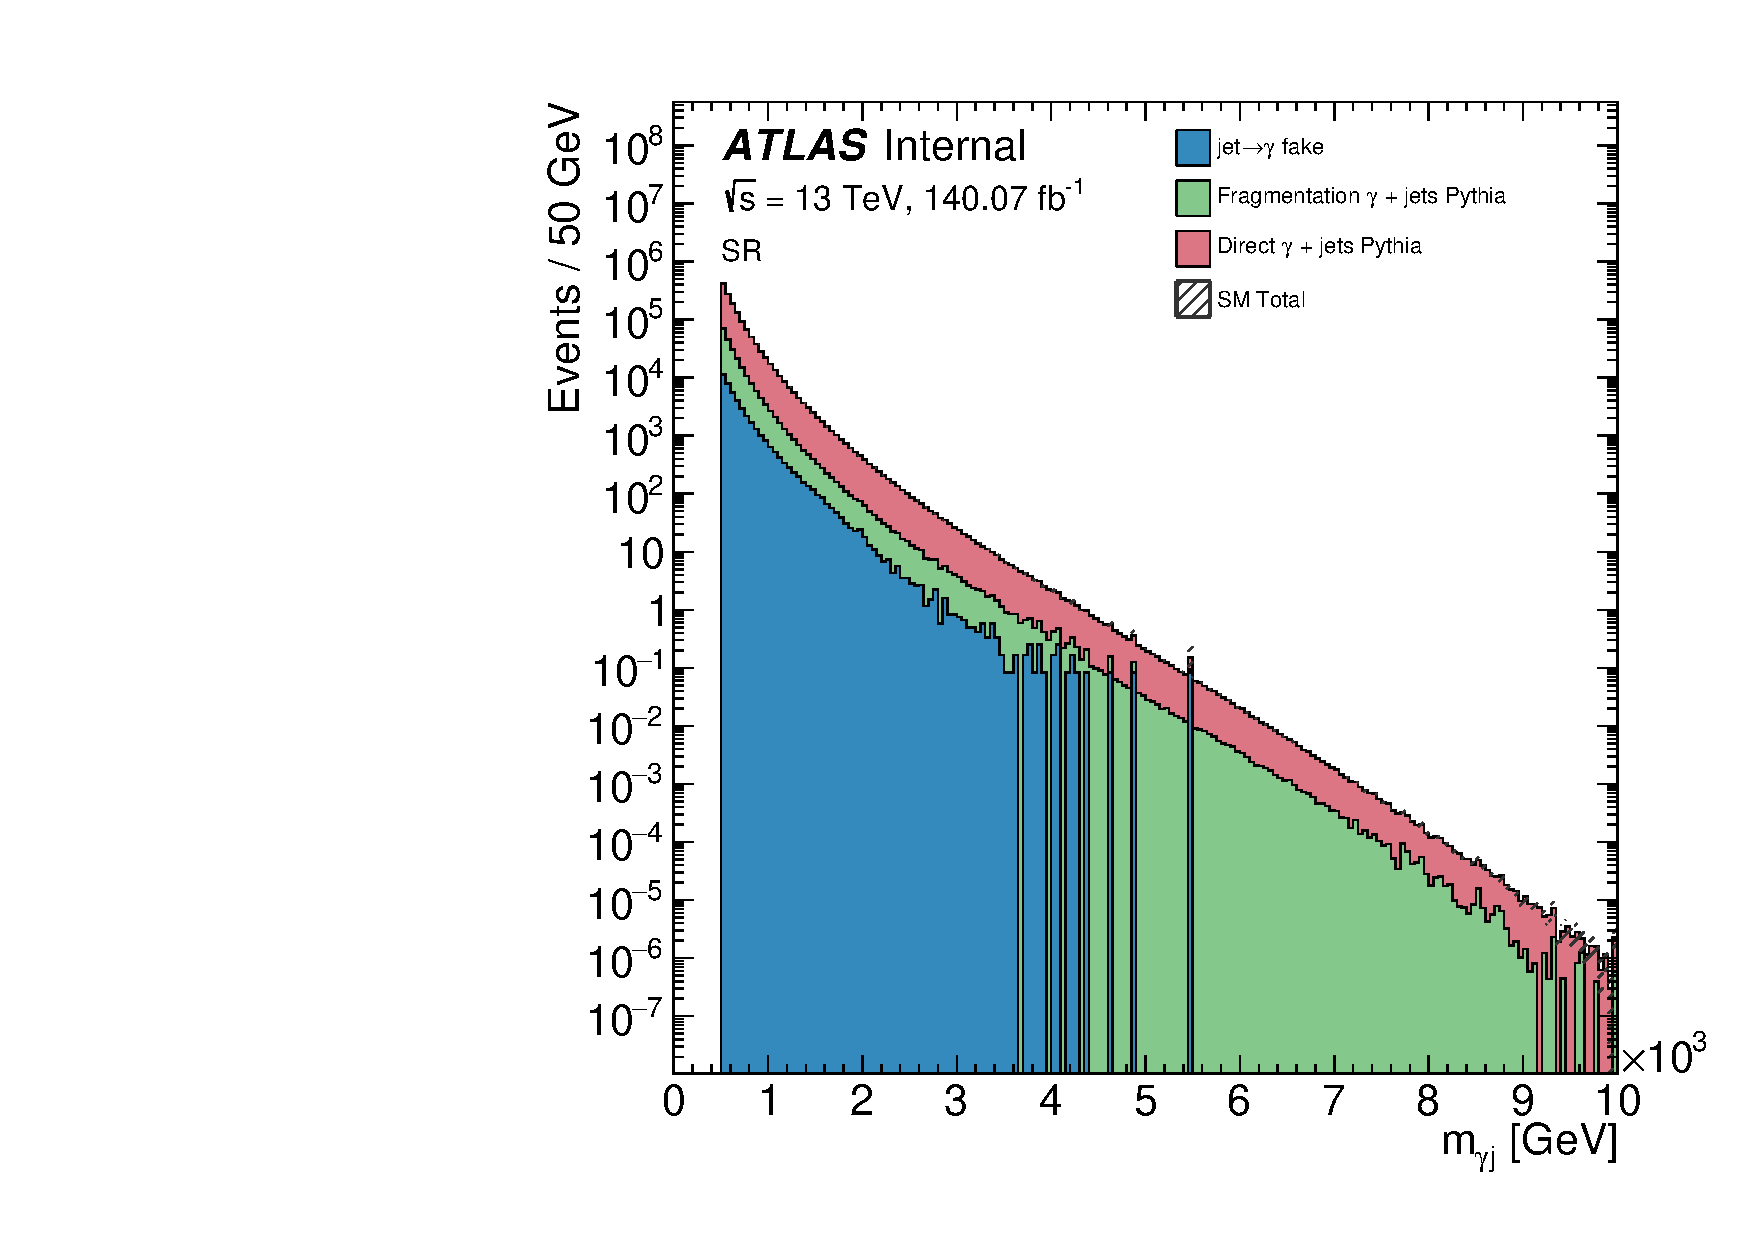
\includegraphics[width=\textwidth]{5_resonances/bkg/modeling/datasets_preparation/jfakes_smoothing/can__photonjet_Pythia_jfakeisosmooth__SR__phjet_m__Run2}
        \caption{SR}
    \end{subfigure}
    \hfill
    \begin{subfigure}[h]{0.49\linewidth}
        \centering
        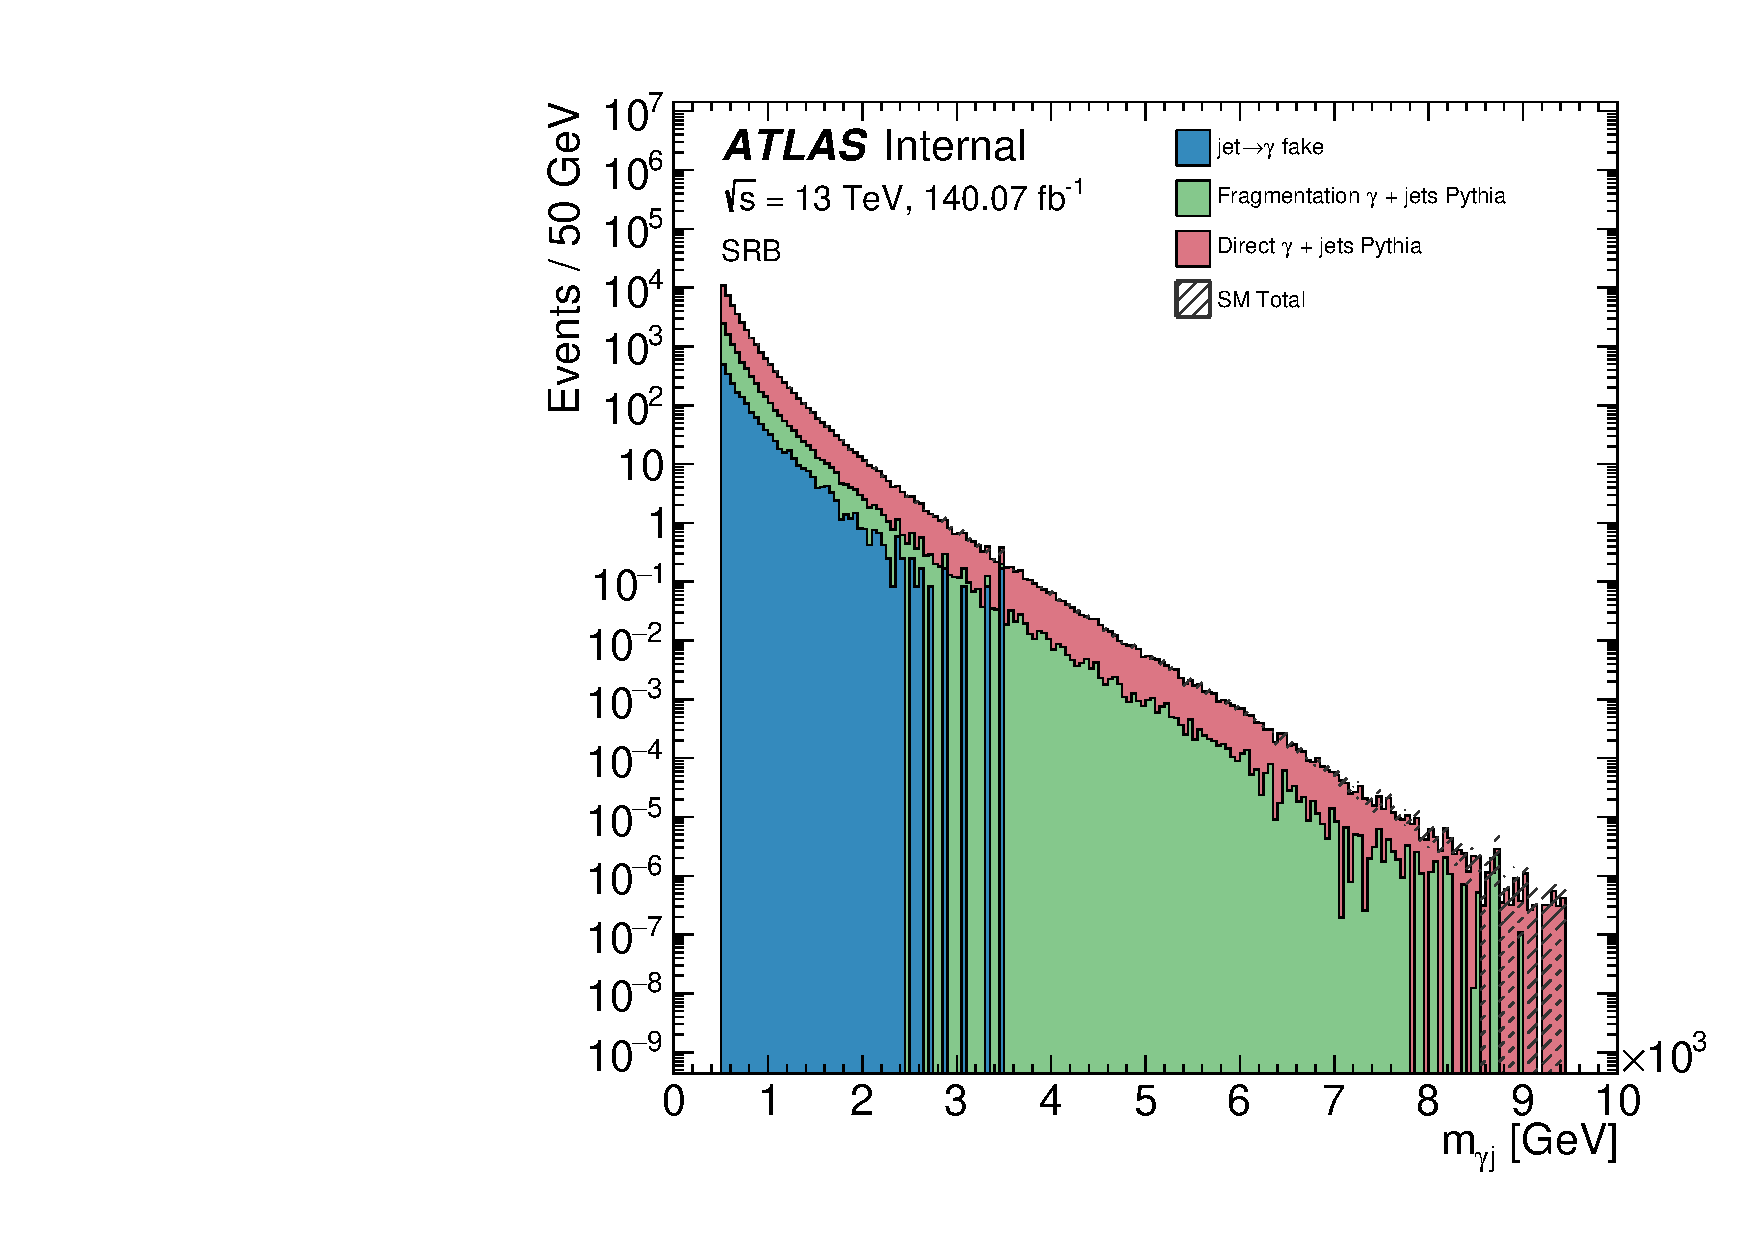
\includegraphics[width=\textwidth]{5_resonances/bkg/modeling/datasets_preparation/jfakes_smoothing/can__photonjet_Pythia_jfakeisosmooth__SRB__phjet_m__Run2}
        \caption{SRB}
    \end{subfigure}\\
    \caption{Distribución de \myj mostrando el efecto de los eventos aislados de fotones falsos que distorsionan la forma total, para las regiones de se\~nal SR y SRB.}
    \label{fig:bkg:modeling:preparation:jfakes_smooth:bkg_myj_distribution}
\end{figure}

Teniendo en cuenta estas razones, se realiza un suavizado del fondo de fotones falsos ajustando su distribución \myj con una función \textit{dof8} que no se utilizará para modelar el fondo combinado.
Los ajustes se realizan en el rango \([500-10000]~\gev\), para evitar el pico de la distribución \myj. Ejemplos de estos ajustes para diferentes regiones de señal se muestran en la \Fig{\ref{fig:bkg:modeling:preparation:jfakes_smooth:jfakes_fits}}, donde en todos los casos se obtienen convergencias en los ajustes.

\begin{figure}[ht!]
    \centering
    \begin{subfigure}[h]{0.49\linewidth}
        \centering
        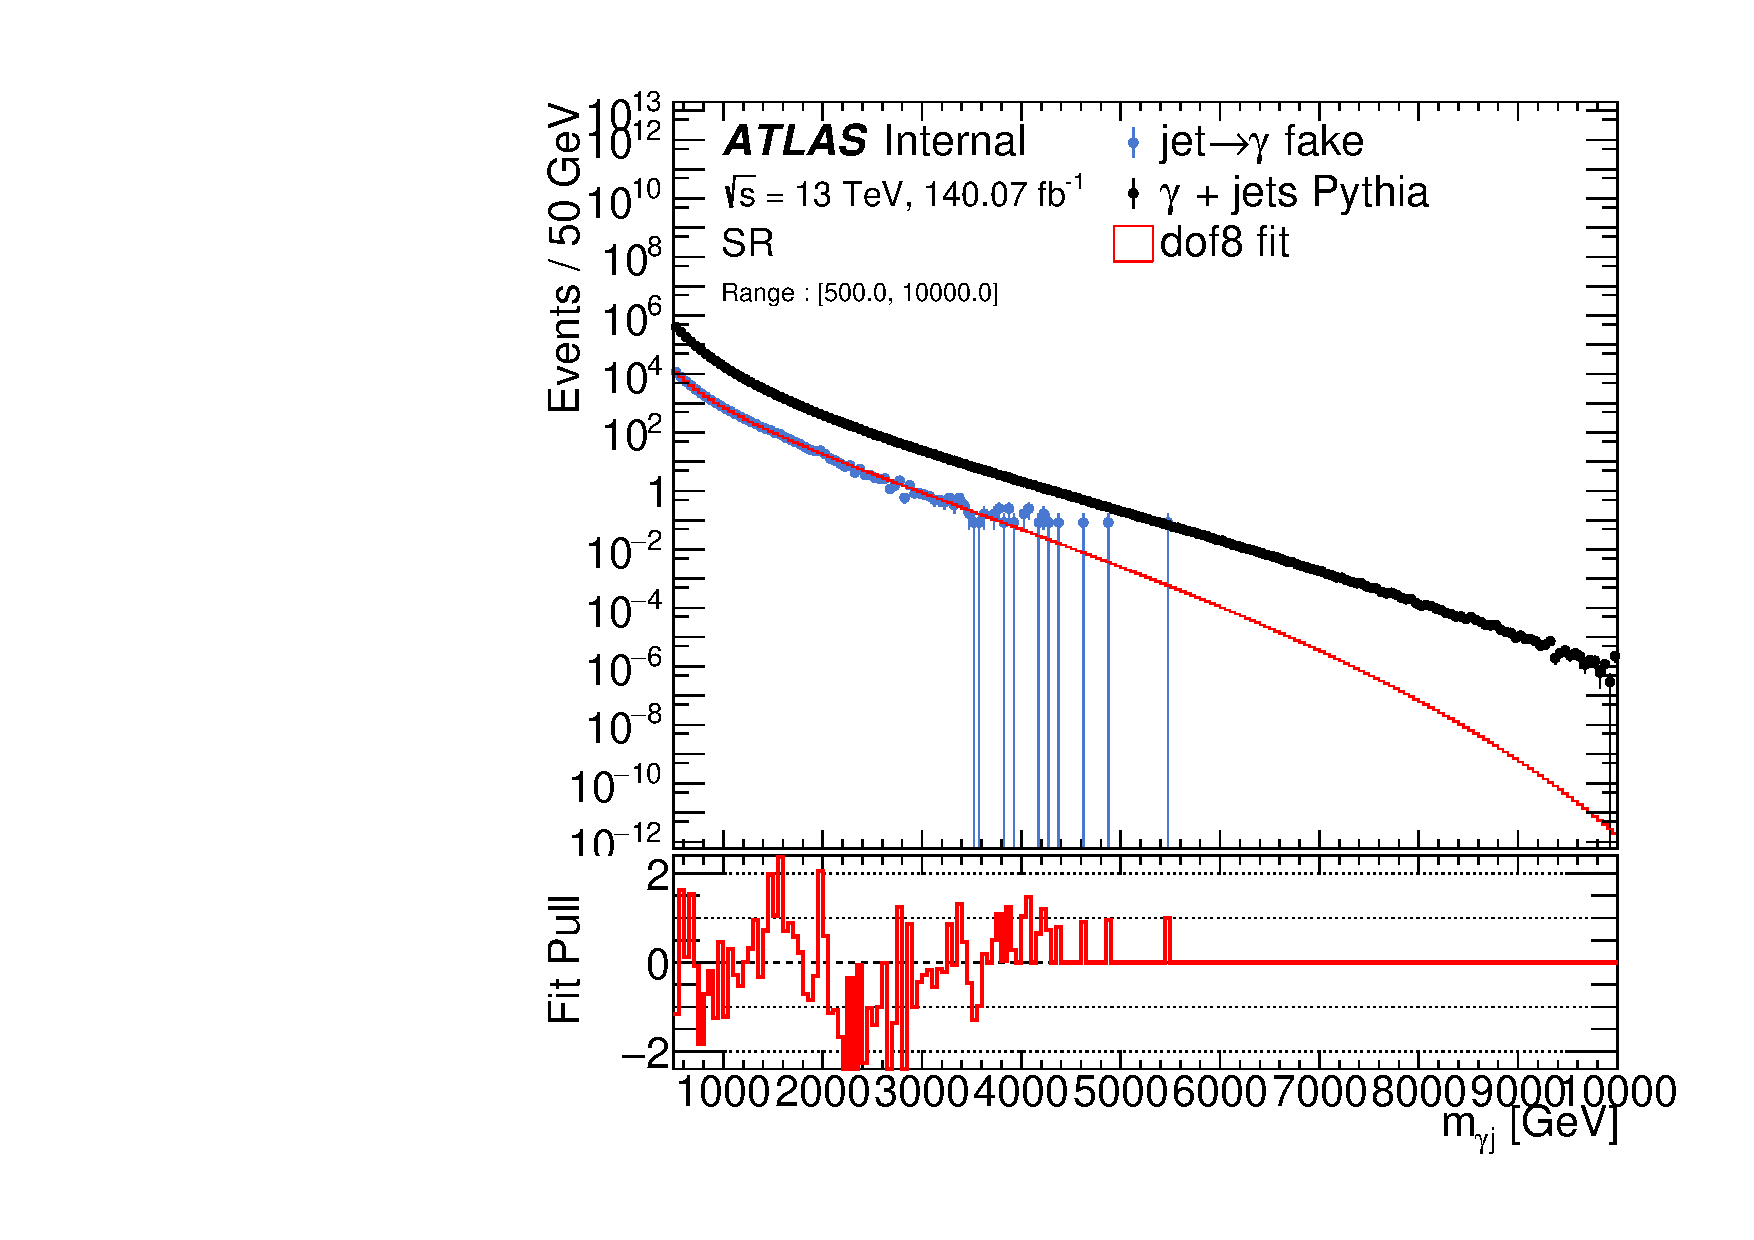
\includegraphics[width=\textwidth]{5_resonances/bkg/modeling/datasets_preparation/jfakes_smoothing/can__jfakes_fit__dof8__SR__range_500-10000}
        \caption{Inclusive SR region}
    \end{subfigure}
    \hfill
    \begin{subfigure}[h]{0.49\linewidth}
        \centering
        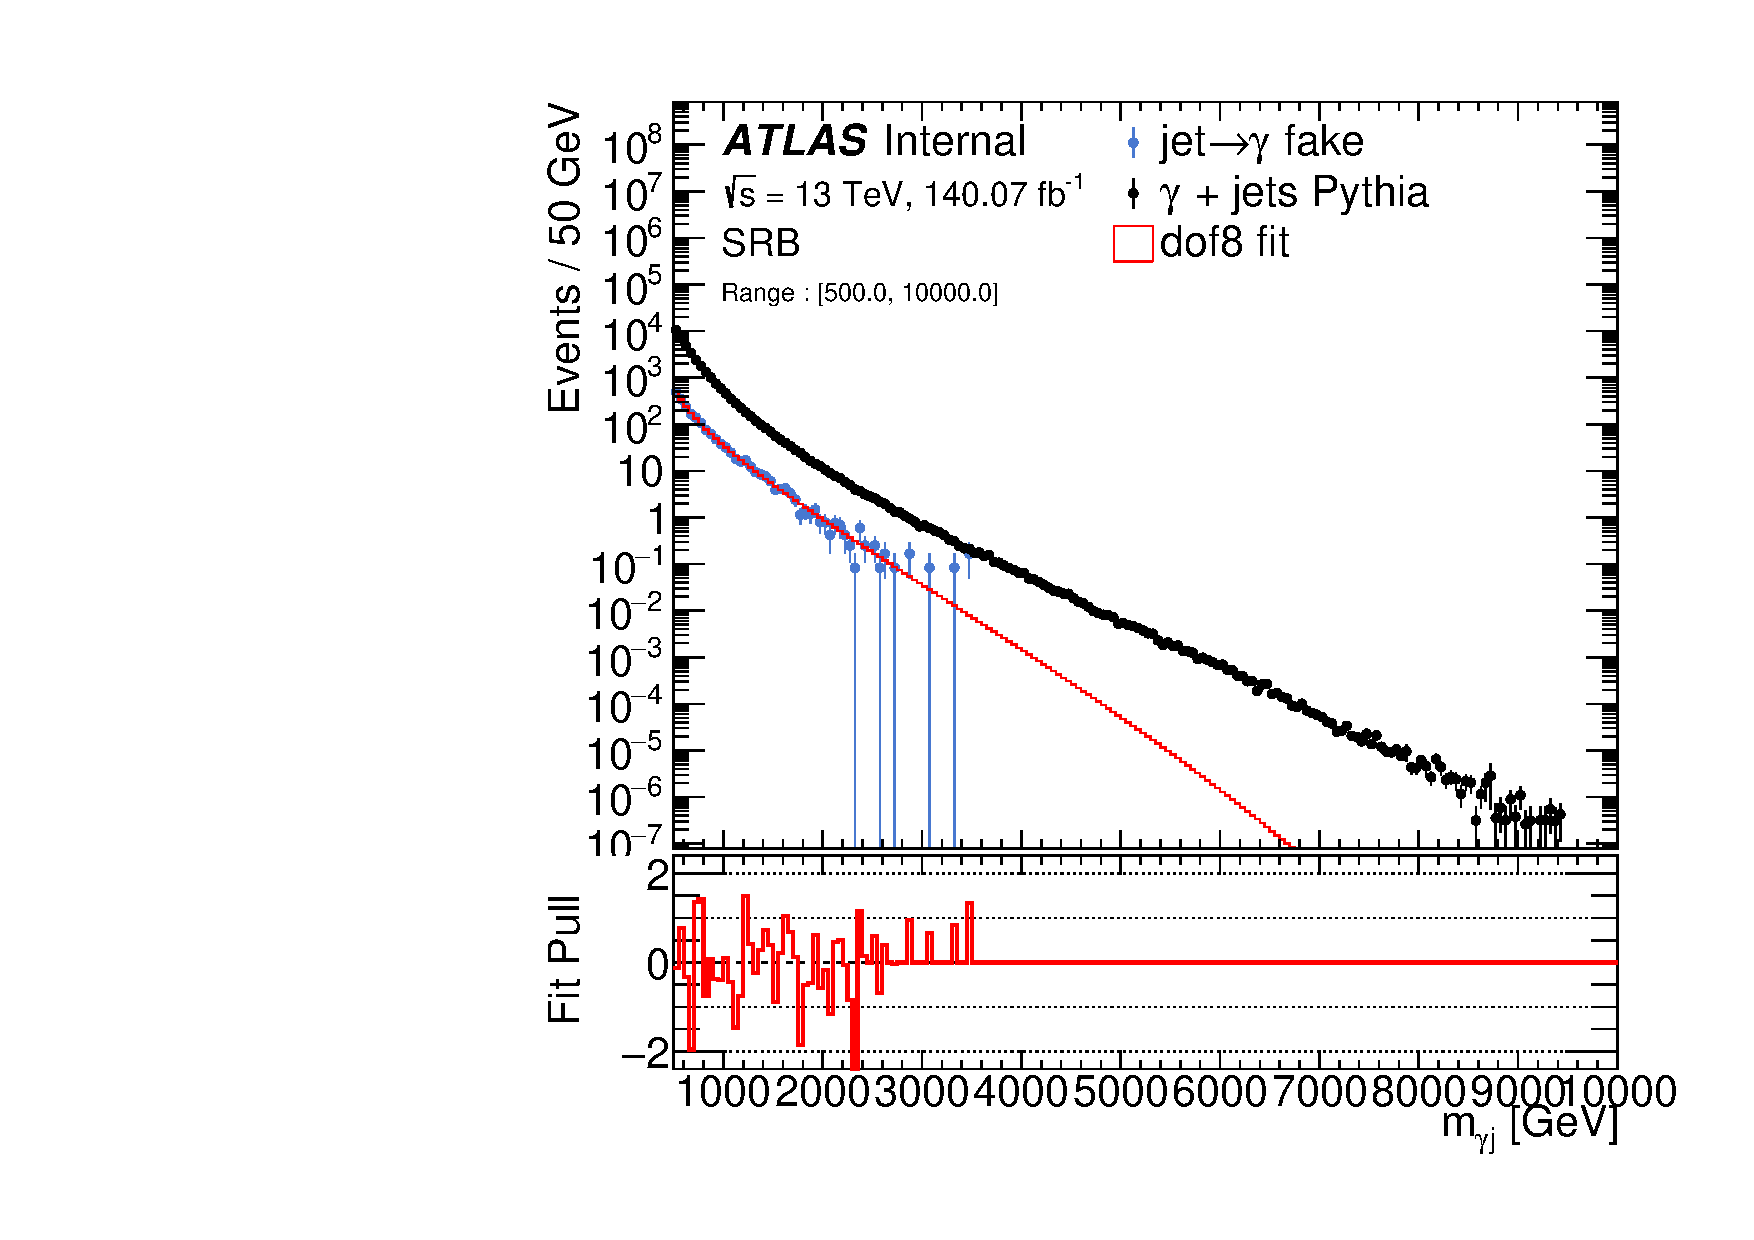
\includegraphics[width=\textwidth]{5_resonances/bkg/modeling/datasets_preparation/jfakes_smoothing/can__jfakes_fit__dof8__SRB__range_500-10000}
        \caption{\btag region, SRB}
    \end{subfigure}
    \caption{Ajustes al fondo de fotones falso utilizando la función \textit{dof8} en diferentes regiones de se\~nal.}
    \label{fig:bkg:modeling:preparation:jfakes_smooth:jfakes_fits}
\end{figure}

Una vez que se ha suavizado la contribución al fondo de los fotones falsos, la función resultante se añade directamente al histograma de \ac{MC} del fondo de \gammajet.







\subsubsection{Muestras Asimov y ajustes de sólo fondo}
\label{subsubsec:bkg:modeling:preparation:asimov_bkgonly}

Un muestra Asimov se define de tal manera que, cuando se utiliza para evaluar los estimadores de todos los parámetros, se obtienen los verdaderos valores de los parámetros:
\begin{equation}
    \hat{x} = x_0
\end{equation}
para todos los parámetros \(x\), donde \(x_0\) es el valor verdadero del parámetro. Estos conjuntos de datos se construyen como histogramas con un binneado muy fino, en la que el el número de eventos en cada bin es el número de eventos esperado.

El fondo de \gammajet se beneficia de tener una gran estadística, lo que lo convierte en la mejor elección para modelar el espectro de masa invariante \gammajet. Por lo tanto, la muestra de \gammajet, con la adición de la distribución de fotones falsos, se ajusta para crear las muestras Asimov. En primer lugar, el contenido de cada uno de los bins se establece en:
\begin{equation}
    n_i = 
    \begin{cases}
        n_i, & n_i > 0\\
        0, & n_i \leq 0
    \end{cases},
\end{equation}
y los errores de los bines son de la forma \(\sqrt{n_i}\), donde \(n_i\) es el número de eventos en el bin \(i\).


Se definen numerosas combinaciones de modelos funcionales (número de \ac{dof}) y rangos de ajuste por región de señal. Además, con el fin de crear muestras de pseudo-datos (o toys, discutidos más adelante) para cada uno de los modelos funcionales y rangos, es importante garantizar que se pueda lograr un ajuste de \ac{BO} con los conjuntos de datos creados previamente.
Para ello, se utilizan las distribuciones de \myj preparadas para crear conjuntos de datos Asimov ajustándolos con los diferentes modelos, utilizando un rango lo suficientemente grande como para acomodar todas las señales que se van a utilizar en el análisis en cada región.

\begin{figure}[ht!]
    \centering
    \begin{subfigure}[h]{0.32\linewidth}
        \centering
        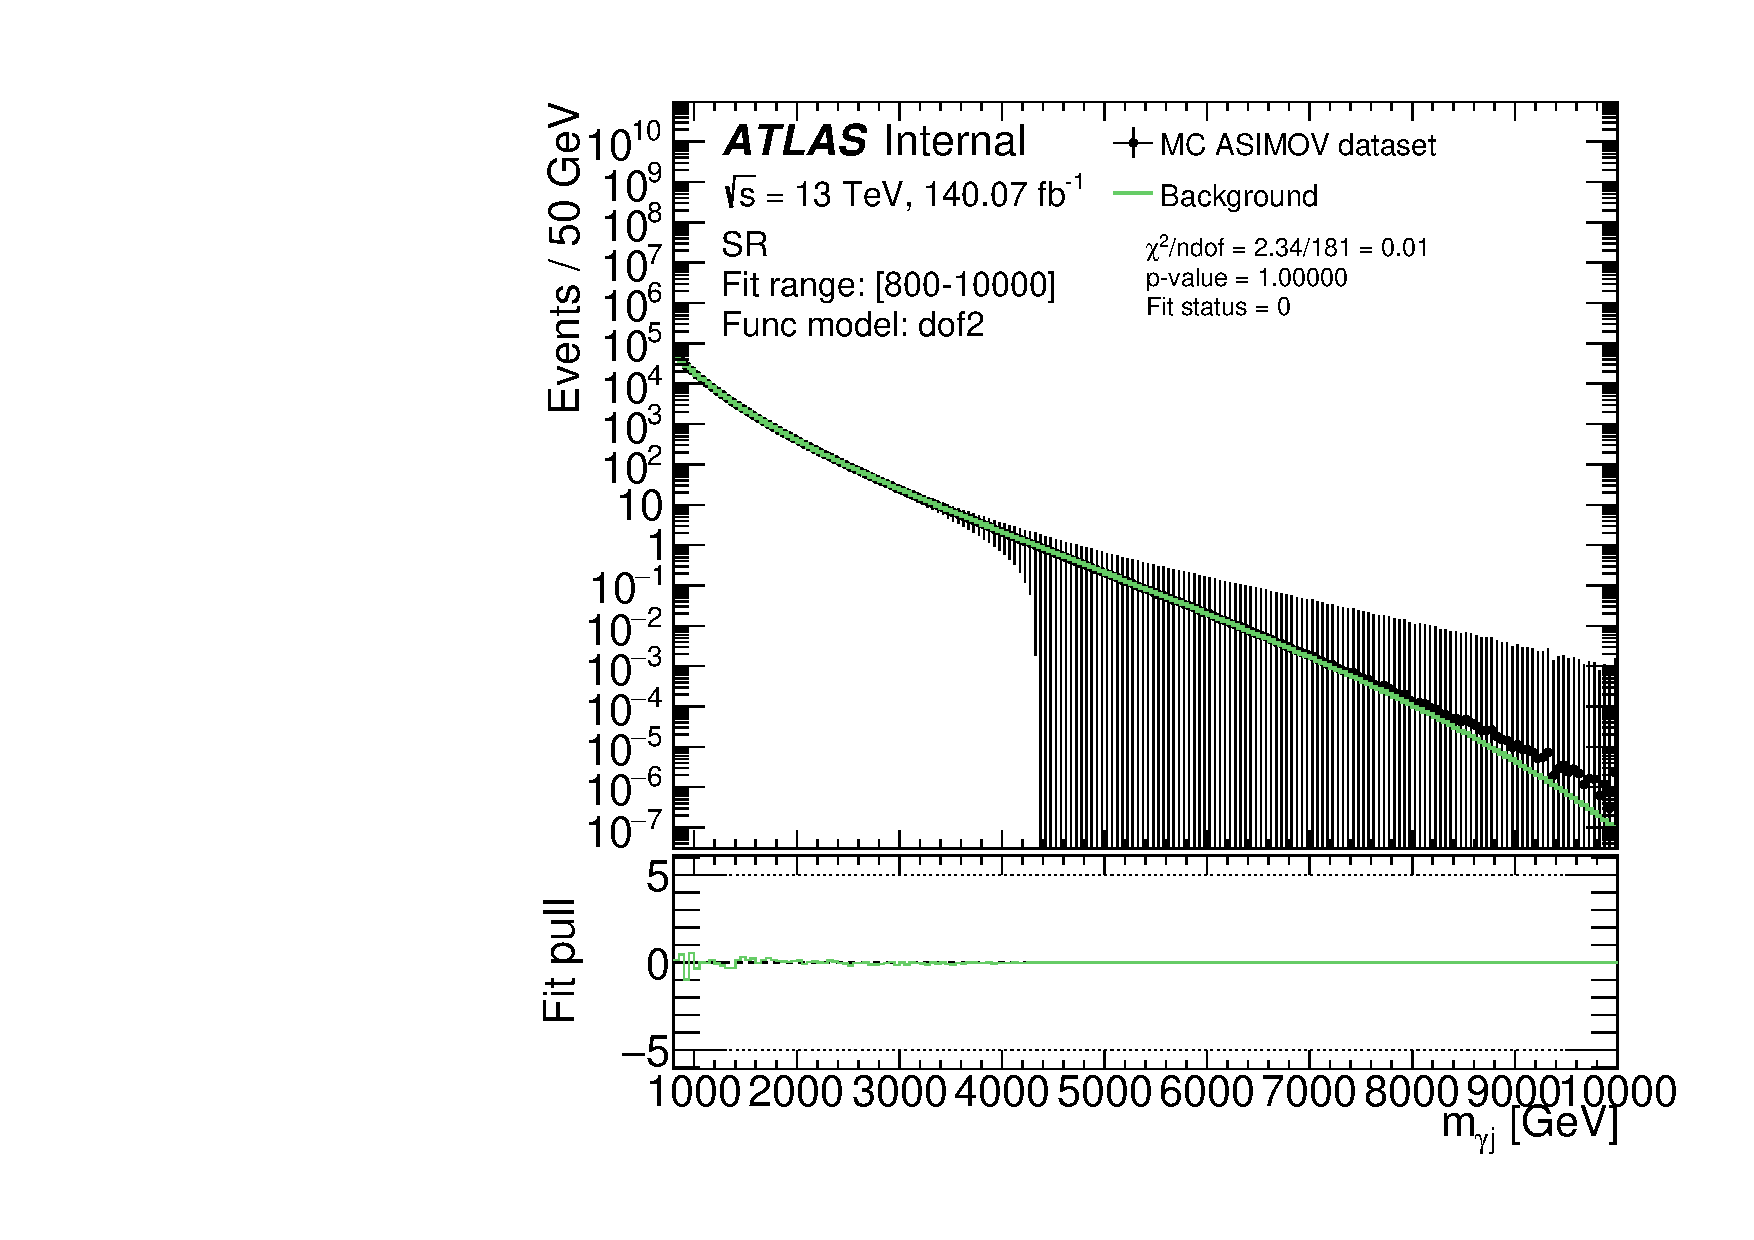
\includegraphics[width=\textwidth]{5_resonances/bkg/modeling/datasets_preparation/fit_hists/SR/can__bkgonlyfit__asimov__photonjet_Pythia__SR__dof2__range_800-10000}
    \end{subfigure}
    \hfill
    \begin{subfigure}[h]{0.32\linewidth}
        \centering
        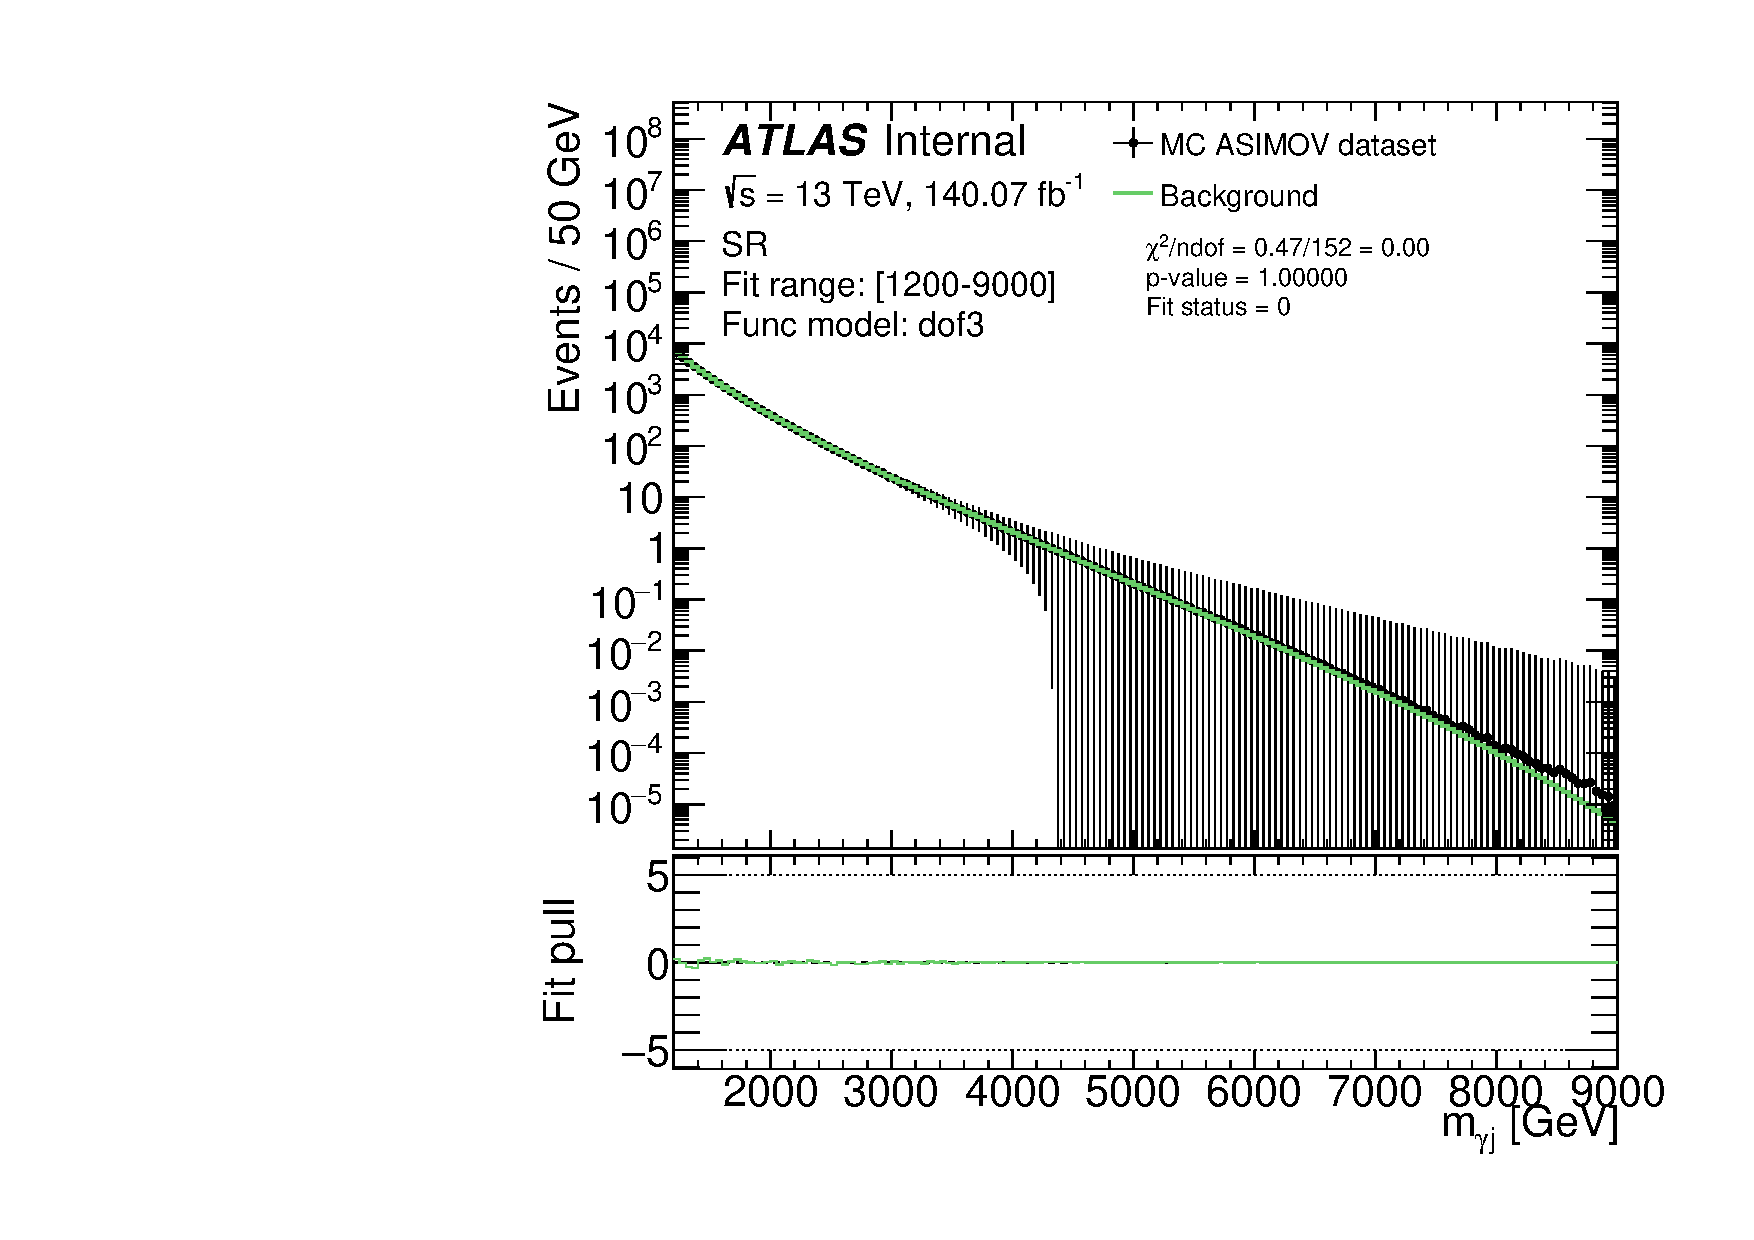
\includegraphics[width=\textwidth]{5_resonances/bkg/modeling/datasets_preparation/fit_hists/SR/can__bkgonlyfit__asimov__photonjet_Pythia__SR__dof3__range_1200-9000}
    \end{subfigure}
    \hfill
    \begin{subfigure}[h]{0.32\linewidth}
        \centering
        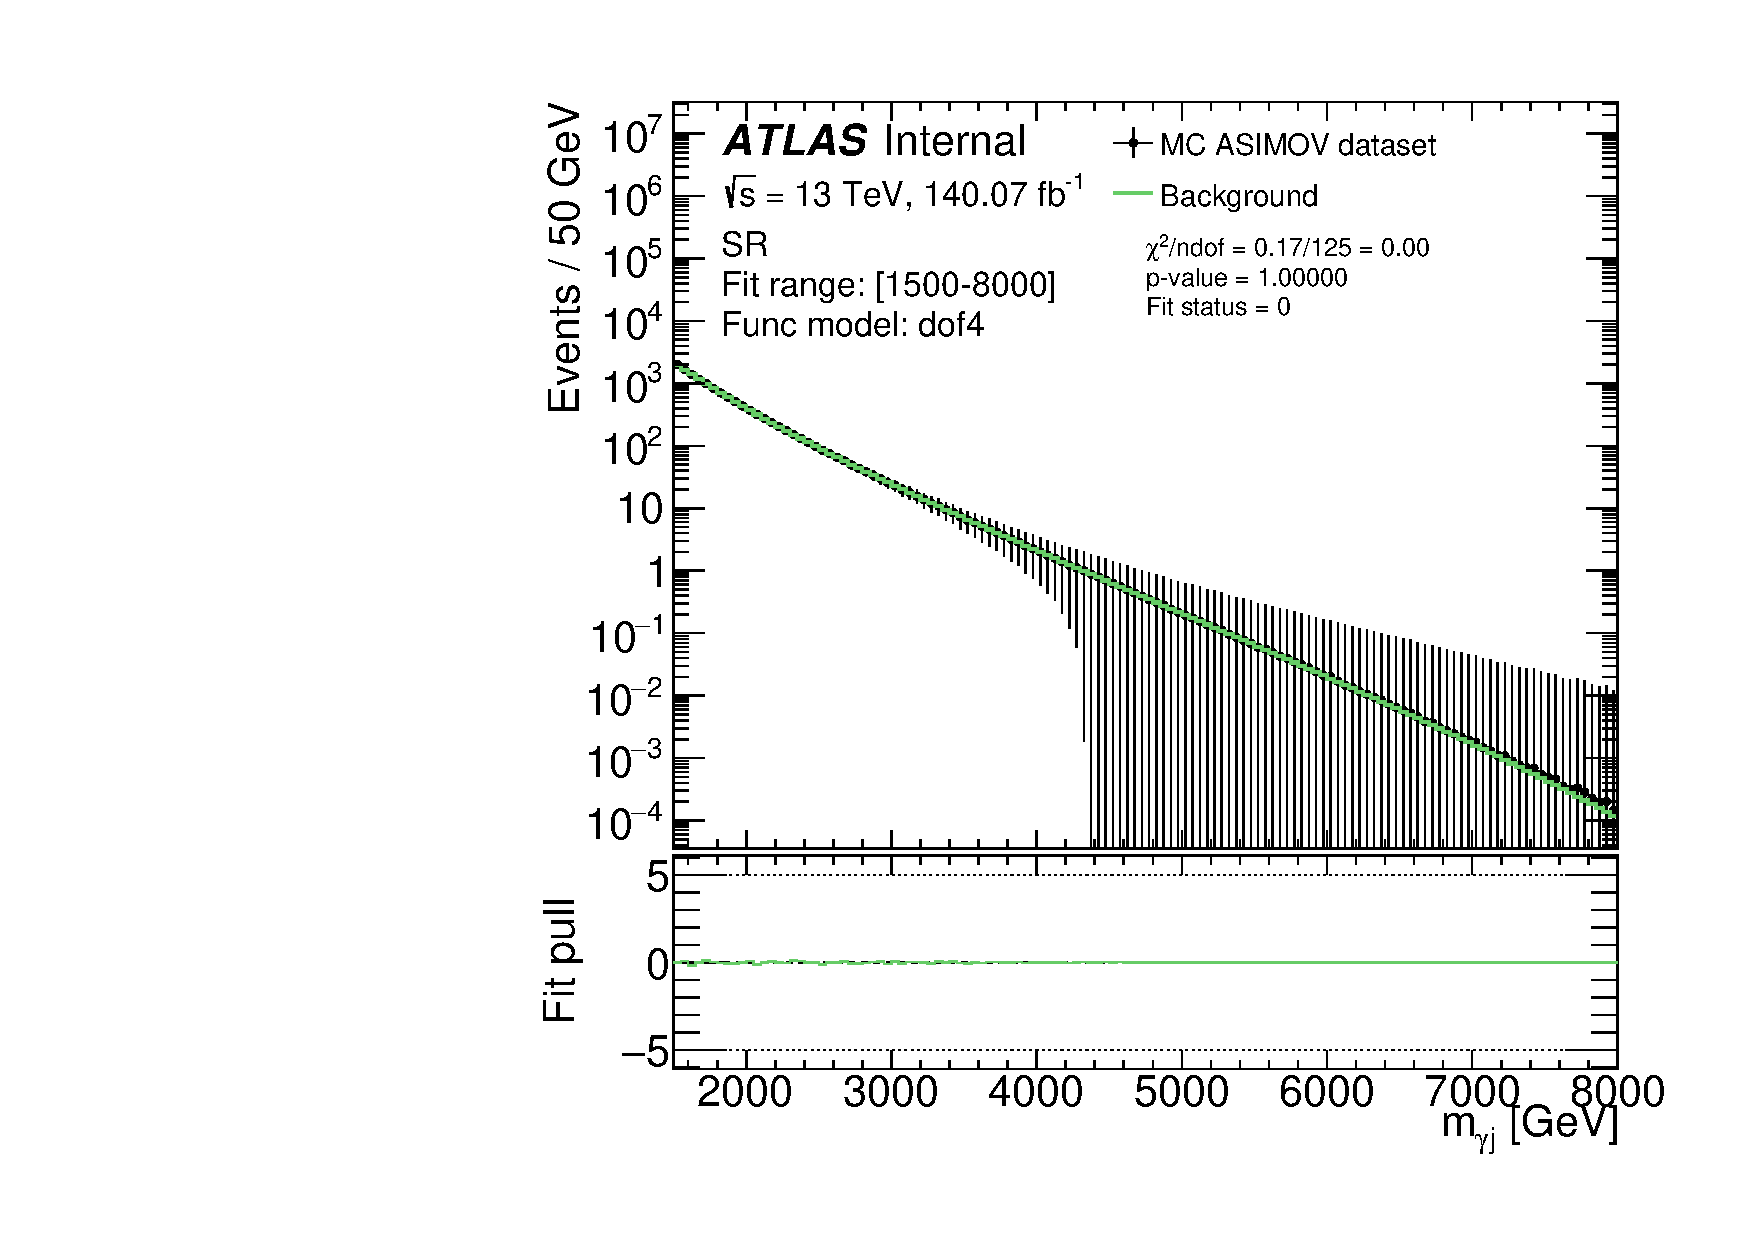
\includegraphics[width=\textwidth]{5_resonances/bkg/modeling/datasets_preparation/fit_hists/SR/can__bkgonlyfit__asimov__photonjet_Pythia__SR__dof4__range_1500-8000}
    \end{subfigure}\\
    \caption{Ajustes de \ac{BO} utilizando diversas funciones y rangos de ajuste en la región inclusiva SR.}
    \label{fig:bkg:modeling:preparation:asimov_bkgonly:bkgonly_fits}
\end{figure}

La \Fig{\ref{fig:bkg:modeling:preparation:asimov_bkgonly:bkgonly_fits}} muestra algunos ejemplos de los ajustes de \ac{BO} en la región SR. Como se puede notar, todas las funciones lograr ajustar bien al fondo, logrando obtener una descripción correcta de el.








\subsubsection{Creación de pseudodatos}
\label{subsubsec:bkg:modeling:preparation:toys}

Los pseudodatos, o también llamados distribuciones \textit{toys}, son esencialmente distribuciones del fondo utilizadas para imitar datos reales. Los toys se calculan a partir de ajustes de \ac{BO} a los conjuntos de datos Asimov, y cada bin de la distribución se calcula como un número aleatorio de Poisson con media \(v_i = n_i\), donde \(n_i\) es el ajuste evaluado en el bin \(i\). Se calculan diferentes conjuntos de distribuciones de toys en función del número de parámetros con los que se haya realizado el ajuste de \ac{BO}. Se genera un total de 500 toys por región de señal y por modelo funcional.

Para probar los ajustes con el modelo \textit{dofn}, se utilizan distribuciones de pseudodatos generadas a partir de un modelo más complejo, \textit{dof(n+1)}. En la \Fig{\ref{fig:bkg:modeling:preparation:toys:bkgonly_examples_toys_fits}}, se muestran dos ejemplos de ajuste a toys. En este caso, los toys se generaron a partir de un ajuste \textit{dof3} al \ac{MC}, y ahora se están ajustando con un modelo \textit{dof2}.

\begin{figure}[ht!]
    \centering
    \begin{subfigure}[h]{0.49\linewidth}
        \centering
        \includegraphics[width=\textwidth, page=123]{5_resonances/bkg/modeling/datasets_preparation/fit_toys/SR/dof2__range_800-10000/can__bkgonlyfit__toys__photonjet_Pythia__SR__dof2__range_800-10000}
    \end{subfigure}
    \hfill
    \begin{subfigure}[h]{0.49\linewidth}
        \centering
        \includegraphics[width=\textwidth, page=432]{5_resonances/bkg/modeling/datasets_preparation/fit_toys/SR/dof2__range_800-10000/can__bkgonlyfit__toys__photonjet_Pythia__SR__dof2__range_800-10000}
    \end{subfigure}\\
    \caption{Ajustes de \ac{BO} a diferentes toys en la region SR.}
    \label{fig:bkg:modeling:preparation:toys:bkgonly_examples_toys_fits}
\end{figure}

\begin{figure}[ht!]
    \centering
    \begin{subfigure}[h]{0.32\linewidth}
        \centering
        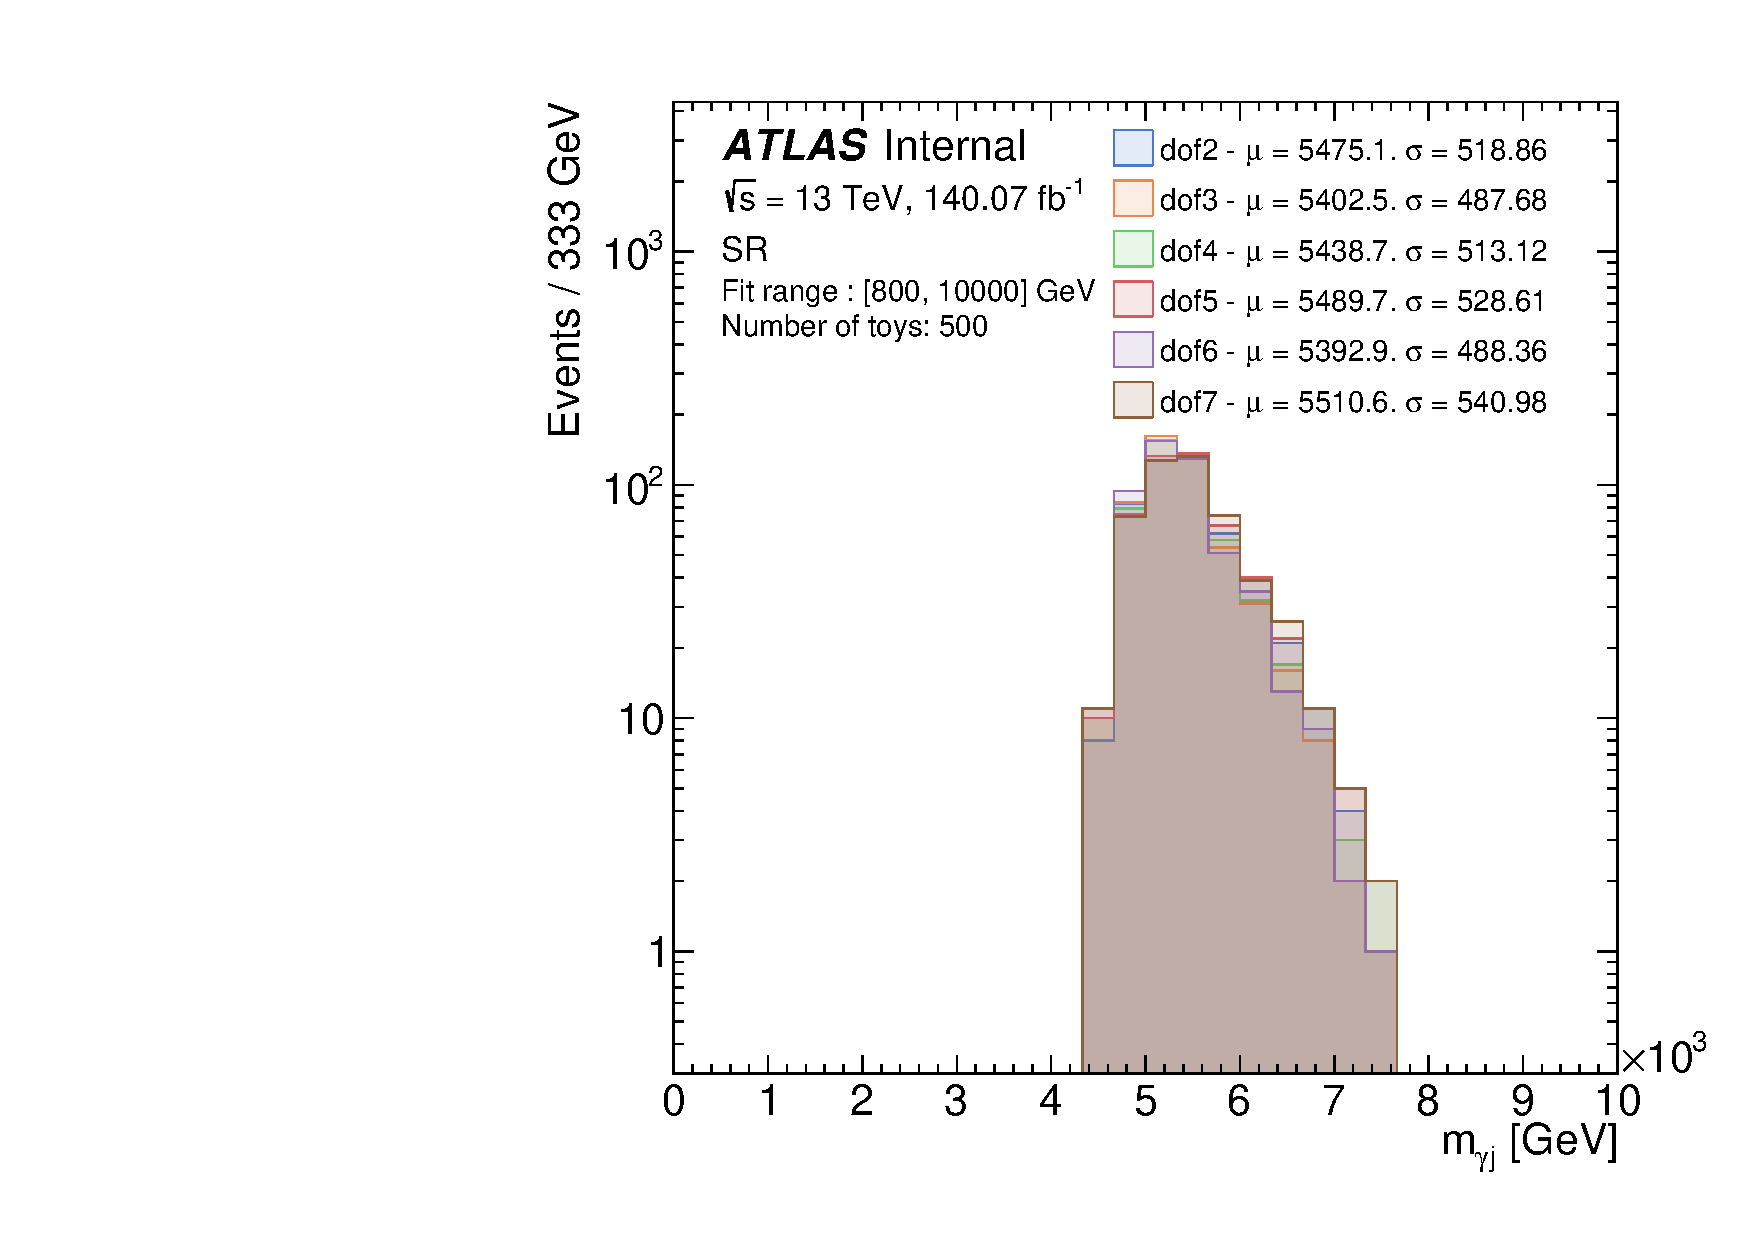
\includegraphics[width=\textwidth]{5_resonances/bkg/modeling/datasets_preparation/fit_toys/maximums/can__bkgPythia__SR__range_800_10000__phjet_m__toys_maximum}
        \caption{SR}
    \end{subfigure}\\
    \begin{subfigure}[h]{0.32\linewidth}
        \centering
        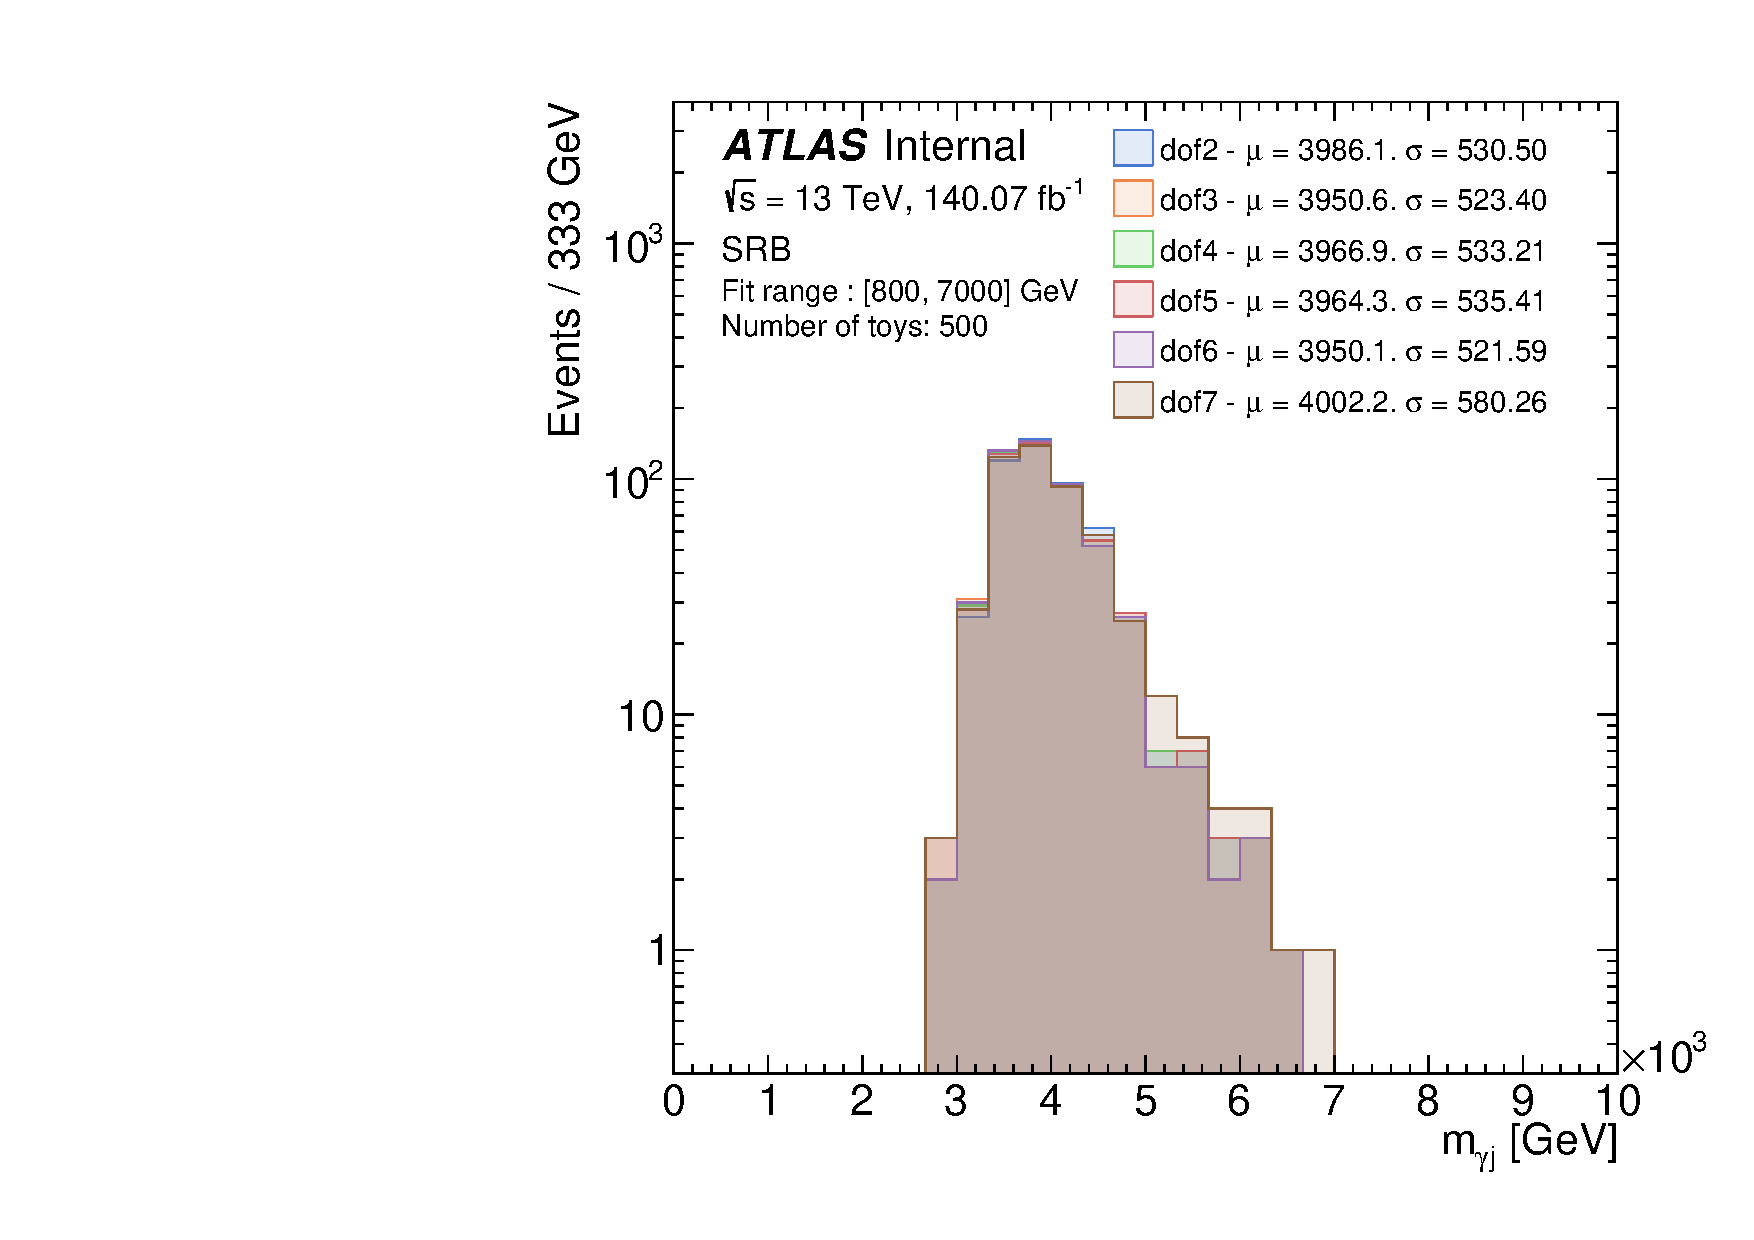
\includegraphics[width=\textwidth]{5_resonances/bkg/modeling/datasets_preparation/fit_toys/maximums/can__bkgPythia__SRB__range_800_7000__phjet_m__toys_maximum}
        \caption{SRB}
    \end{subfigure}
    \begin{subfigure}[h]{0.32\linewidth}
        \centering
        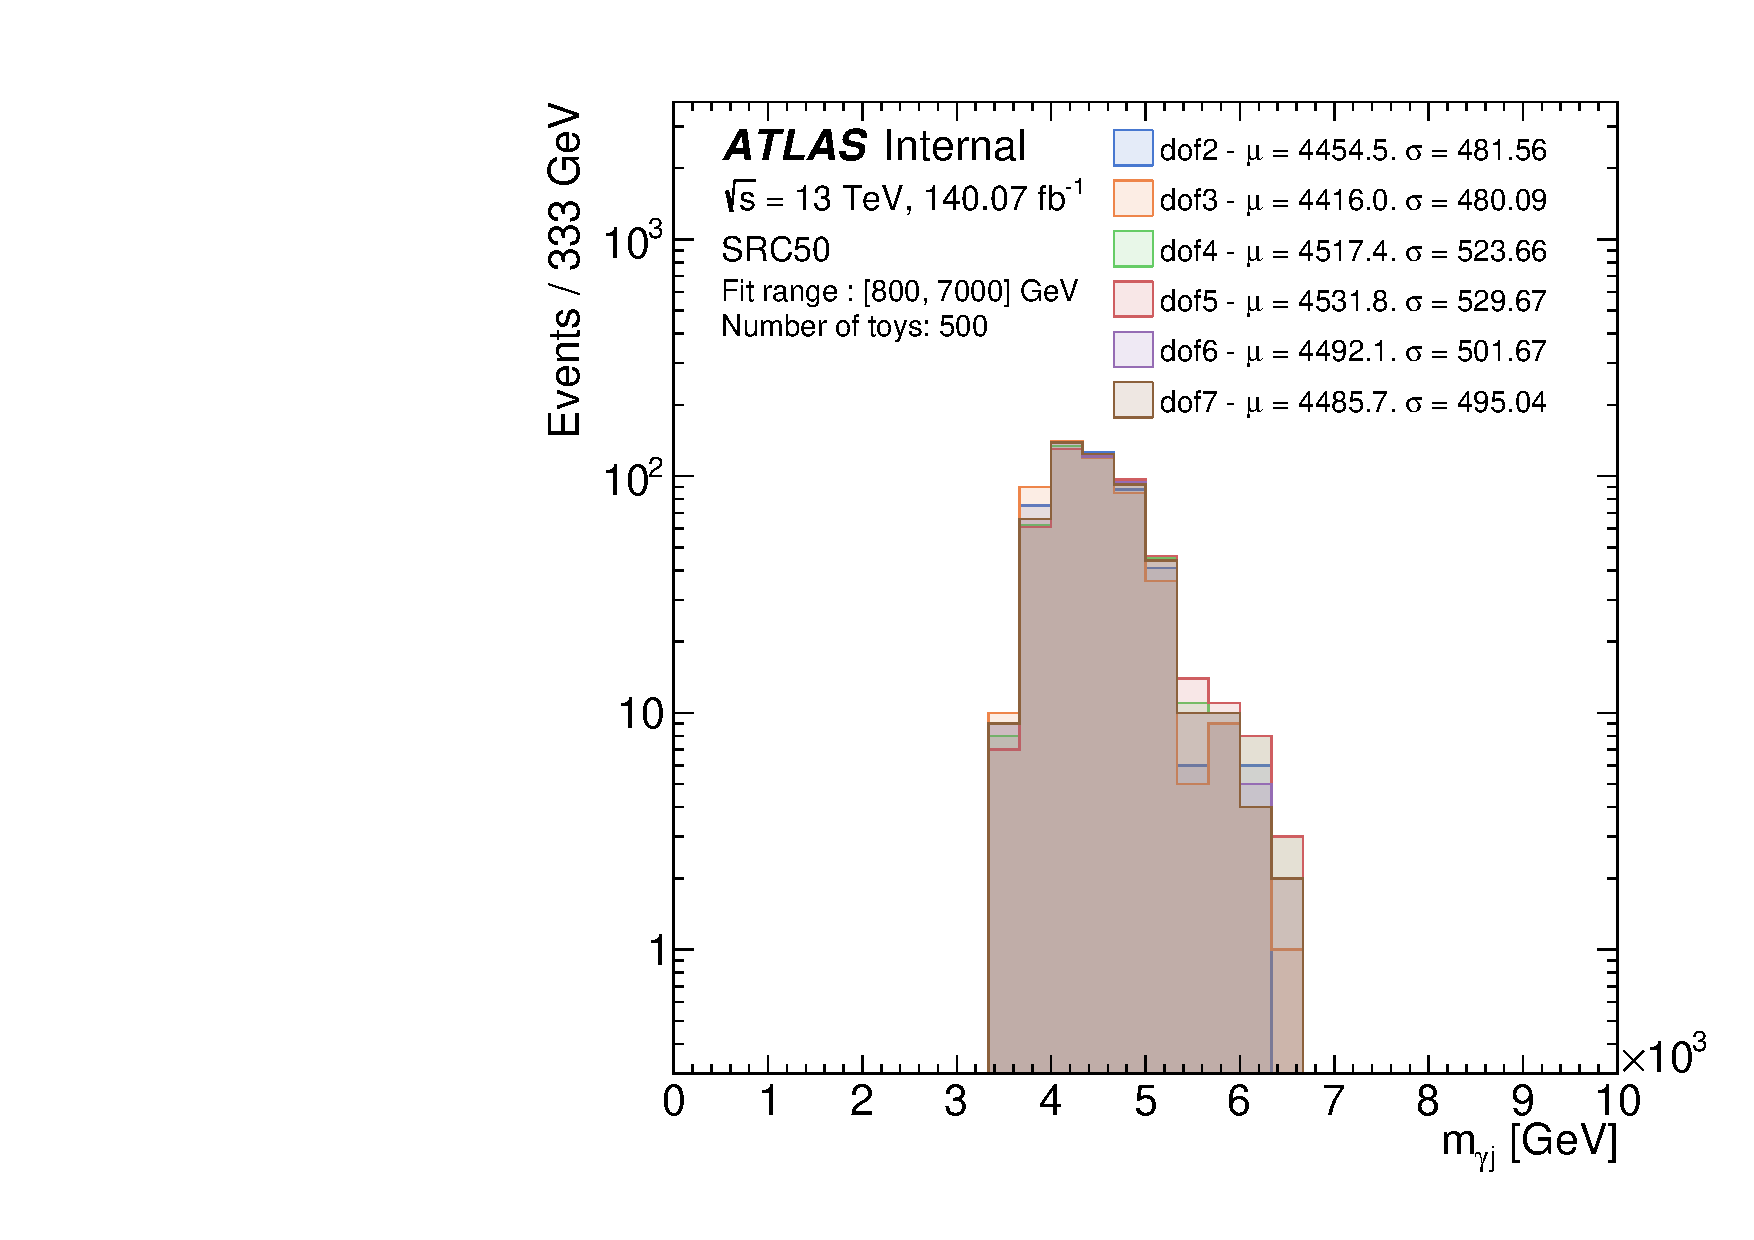
\includegraphics[width=\textwidth]{5_resonances/bkg/modeling/datasets_preparation/fit_toys/maximums/can__bkgPythia__SRC50__range_800_7000__phjet_m__toys_maximum}
        \caption{SRC}
    \end{subfigure}
    \begin{subfigure}[h]{0.32\linewidth}
        \centering
        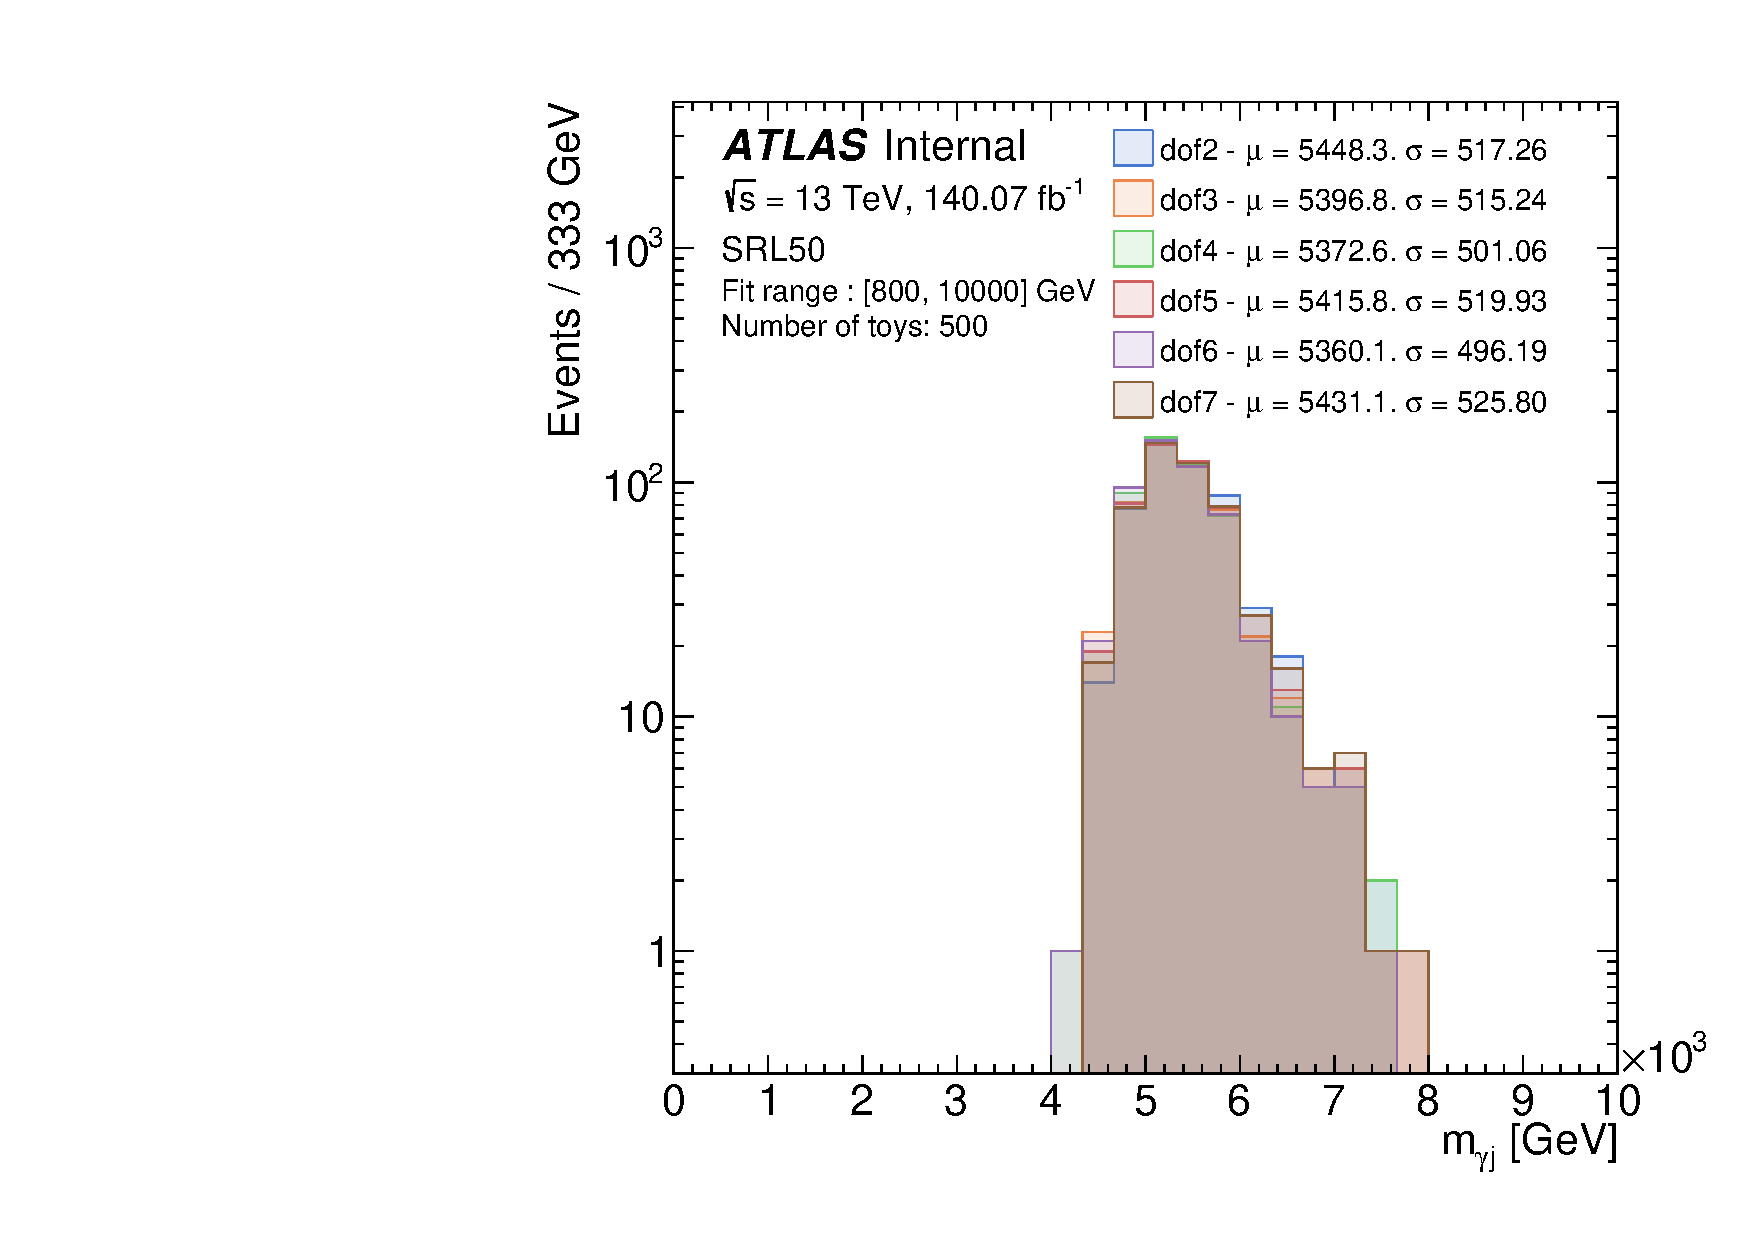
\includegraphics[width=\textwidth]{5_resonances/bkg/modeling/datasets_preparation/fit_toys/maximums/can__bkgPythia__SRL50__range_800_10000__phjet_m__toys_maximum}
        \caption{SRL}
    \end{subfigure}\\
    \caption{Distribuciones del máximo de valor de \myj observado de las muestras de pseudodatos en cada región del análisis considerada. Se muestran diferentes distribuciones para cada uno de los modelos funcionales considerados. Para cada uno de ellos, se muestra el valor medio y la desviación estándar de la distribución.}
    \label{fig:bkg:modeling:preparation:toys:toys_maximums}
\end{figure}

Como ya se ha dicho, las distribuciones de los toys están hechas para imitar el comportamiento que tendrían los datos reales. Para tener una primera aproximación al valor máximo de \myj que se puede obtener, en la \Fig{\ref{fig:bkg:modeling:preparation:toys:toys_maximums}} se muestra la distribución del valor máximo observado de \myj, para cada conjunto de toy generado a partir de los diferentes modelos funcionales. Para cualquiera de las regiones dominadas por \ljets, el valor máximo de \myj se sitúa aproximadamente en \(\sim 5500~\gev\) y la cola derecha se extiende hasta \(\sim 8000~\gev\). Del mismo modo, para las regiones \cjets y \bjets, hay eventos de toys hasta \(\sim 6~\tev\), con la media en \(\sim 4~\tev\). Por estas razones, es importante que el límite superior de los rangos de ajuste sea siempre superior al último evento presente.
























\subsection{Estrategia para definir la función de ajuste}
\label{subsec:bkg:modeling:strategy}


\begin{figure}[ht!]
    \centering
    \begin{subfigure}[t]{0.49\linewidth}
        \centering
        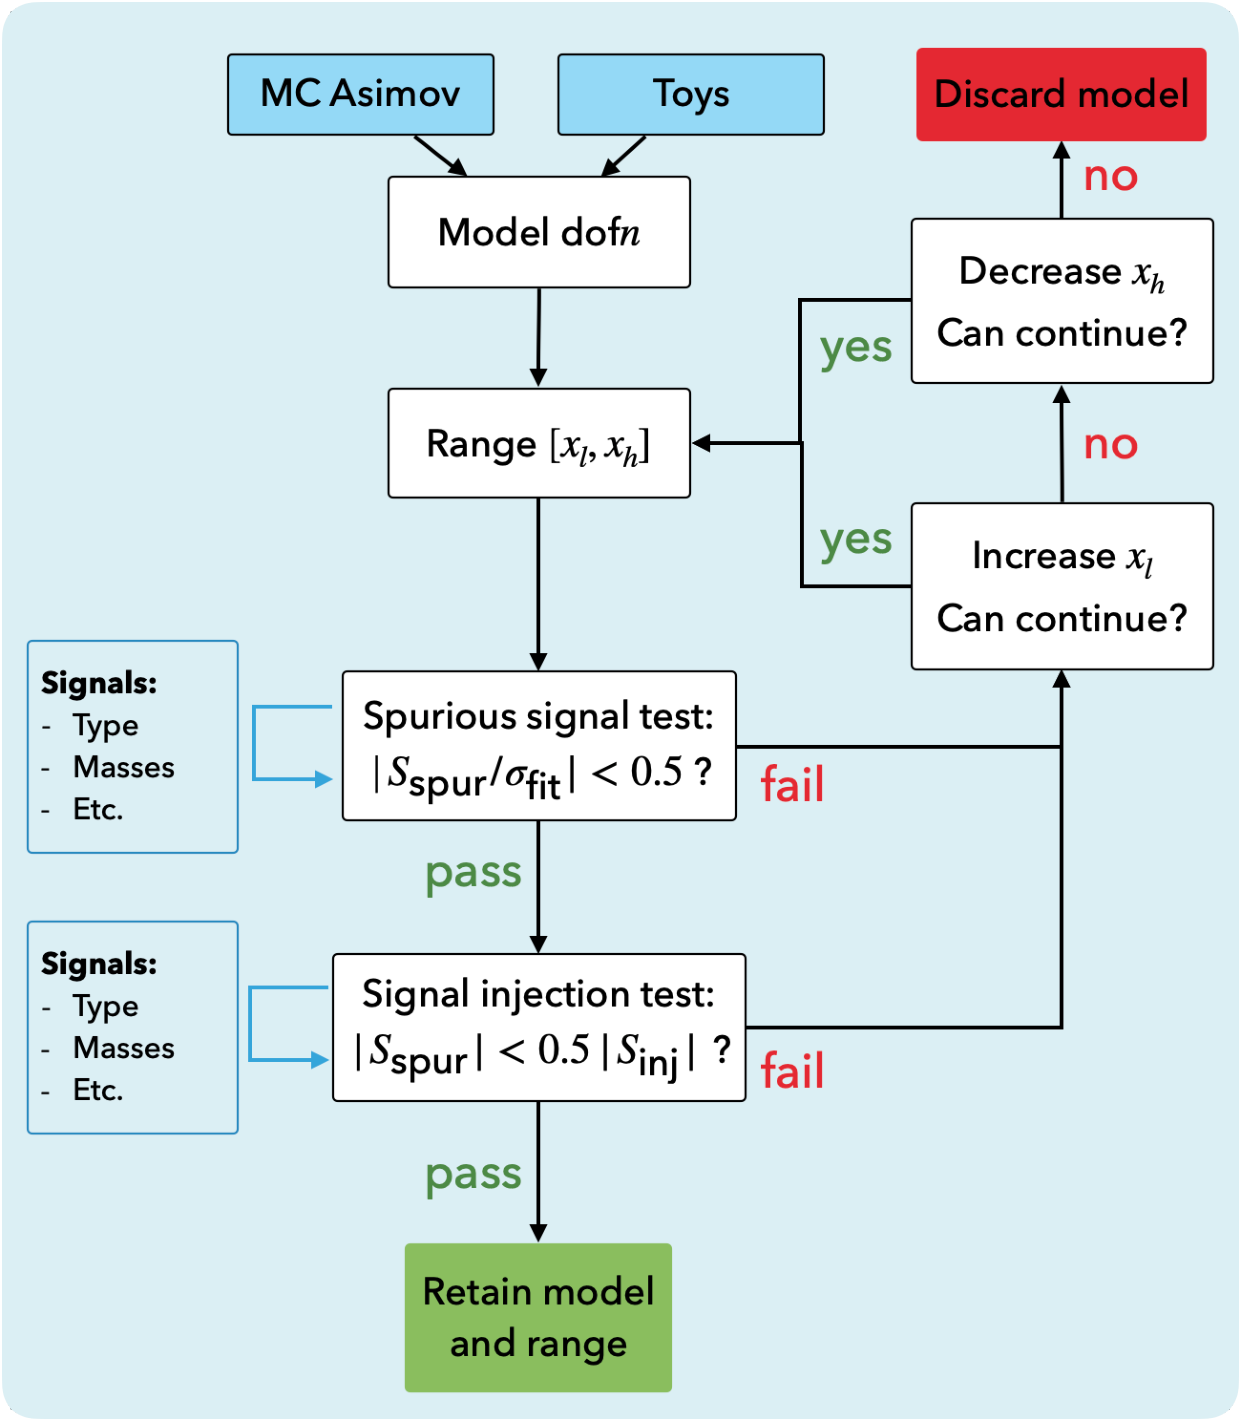
\includegraphics[width=\textwidth]{5_resonances/bkg/modeling/fitmodel_validation}
        \caption{Proceso para la validación de la función y el rango de ajuste mediante los tests de \ac{SSig} e \ac{SI}.}
        \label{fig:bkg:modeling:strategy:validation:tests}
    \end{subfigure}
    \hfill
    \begin{subfigure}[t]{0.49\linewidth}
        \centering
        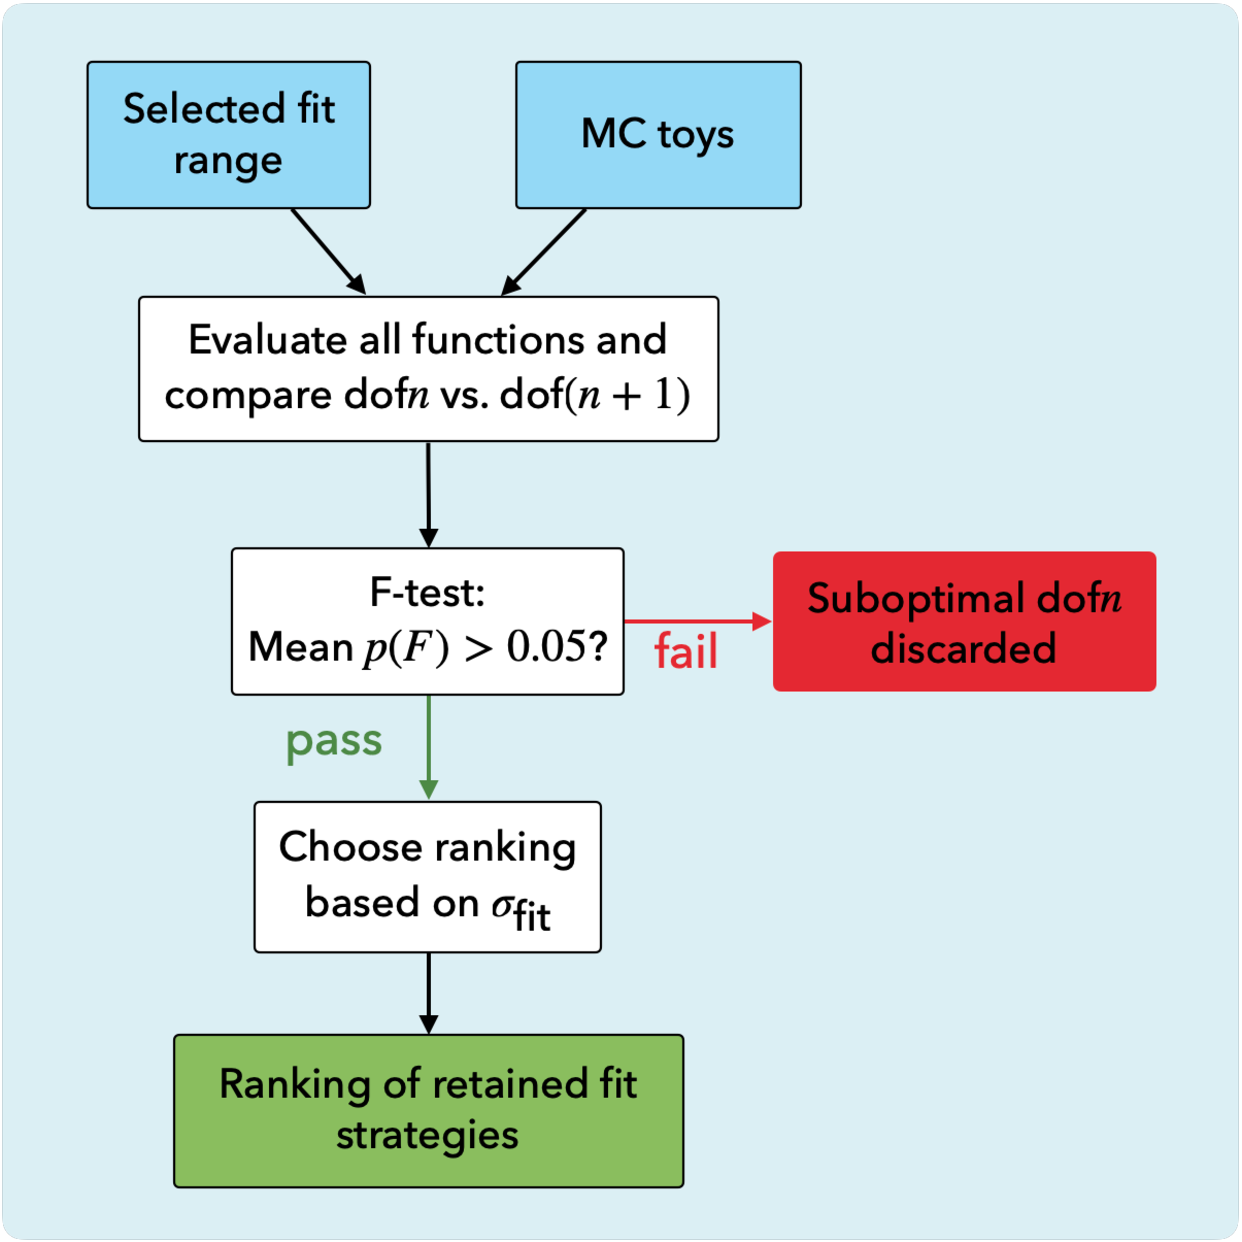
\includegraphics[width=\textwidth]{5_resonances/bkg/modeling/unblind_strategy2}
        \caption{Esquema de la selección de la función óptima basado en el test-\(F\).}
        \label{fig:bkg:modeling:strategy:validation:function_selection}
    \end{subfigure}
    \caption{Proceso para la validación de la función y el rango de ajuste.}
    \label{fig:bkg:modeling:strategy:validation}
\end{figure}

En la \Fig{\ref{fig:bkg:modeling:strategy:validation:tests}} se esquematiza el proceso de selección de una combinación óptima del modelo funcional y el rango del ajuste.
El proceso de validación se lleva a cabo con muestras de \ac{MC}, para ambas muestras creadas, toys y Asimov. Como primer paso, los ajustes de \ac{BO} a la muestra de Asimov deben superar los requisitos indicados en la \Fig{\ref{fig:bkg:modeling:preparation:datasets_generation}} (\(p(\chisq) > 0.05\)) y, a continuación, se obtienen los toys. El primer test al que se someten las muestras es el test de \acf{SSig}. Los modelos y rangos que superan este test se utilizan para los tests de \acf{SI}. En caso de que todos ellos se superen, la función de ajuste se guarda y se somete a otro test, que se describe a continuación. Hay casos en los que los modelos funcionales no cumplen estos requisitos. Para tratar esos casos, el primer paso consiste en aumentar el límite inferior del ajuste, y se vuelve a realizar todo el procedimiento. Cuando ya no se puede aumentar el límite inferior, se puede disminuir el límite superior, teniendo en cuenta que es necesario acomodar todos los modelos de señal. Para cada uno de los tests mencionadas anteriormente, se presenta una explicación completa con los resultados en las secciones siguientes.

Con las funciones y los rangos de ajuste seleccionados, la elección de la función se realiza en función del test-\(F\), y se crea una clasificación de los modelos y rangos de ajuste en función de la \ac{SSig}. Este proceso se encuentra esquematizado en la \Fig{\ref{fig:bkg:modeling:strategy:validation:function_selection}}.







































\subsection{Validación de la estrategia de ajuste}
\label{subsec:bkg:modeling:sigbkg}

En las siguientes secciones, se presenta un análisis detallado de cada parte del proceso de modelización del fondo. Como se indicó anteriormente, el proceso comienza realizando los tests de \ac{SSig} e \ac{SI}, para reunir primero las posibles funciones y rangos de ajuste que se utilizarán en los ajustes finales a los datos. Estas combinaciones de rango-función se clasifican en función del valor de la \ac{SSig}. Por último, se utiliza el test-\(F\) para reordenar estas combinaciones.


\subsubsection{Tests de \acl{SSig}}
\label{subsubsec:bkg:modeling:sigbkg:sstest}

El sesgo en el ajuste, o \acf{SSig}, se estima ajustando una distribución de \ac{BO} con un modelo combinado de \ac{SB}, en el que una de las componentes es la distribución de la señal (o una función gaussiana), y la componente de fondo son las distintas funciones evaluadas.
La \ac{SSig} (\sspur) y su incerteza (\(\sigma_{\text{fit}}\)) se obtienen a partir del númer de eventos de la señal resultante (\(N_{\text{sig}}\)) tras el ajuste a la distribución de \ac{BO}. En un caso ideal, \sspur debería aproximarse a cero, lo que indica que el modelo funcional seleccionado para el fondo captura correctamente toda la distribución.
La \ac{SSig} también puede calcularse a partir de los ajustes a las distribuciones de los toys. En tales casos, \sspur es el valor medio de todos los ajustes realizados a los toys, y \(\sigma_{\text{fit}}\) se calcula como la el ancho de la distribución \sspur. Por tanto, las dos definiciones del valor \ac{SS} son:
\begin{equation}
    \label{eq:bkg:modeling:sigbkg:sstest:sspur_definition_sstest}
    \sspur = 
    \begin{cases}
        N_{\text{sig}} & \qif \text{Asimov dataset},\\
        \expval{N_{\text{sig}}}_{\text{toys}} & \qif \text{Toys dataset}.
    \end{cases}
\end{equation}

El cálculo se realiza para cada una de las masas de señal para cada modelo, en cada una de las regiones de señal. La distribución de \ac{BO} puede ser el conjunto de datos Asimov o todas las distribuciones de los toys. En la \Fig{\ref{fig:bkg:modeling:sigbkg:sstest:sstest_asimov_examples}}, se muestran dos ejemplos de ajustes a la muestra de Asimov para la región inclusiva SR. Los modelos de señal tenidos en cuenta son ambos \qstar con \(f=1.0\) y utilizando las masas \(\mq = 2000~\gev\) y \(\mq = 6000~\gev\). El modelo funcional utilizado para modelar el fondo es el modelo \textit{dof2} y el ajuste se realiza en el rango \myj de \(800-10000~\gev\).

\begin{figure}[ht!]
    \centering
    \begin{subfigure}[h]{0.49\linewidth}
        \centering
        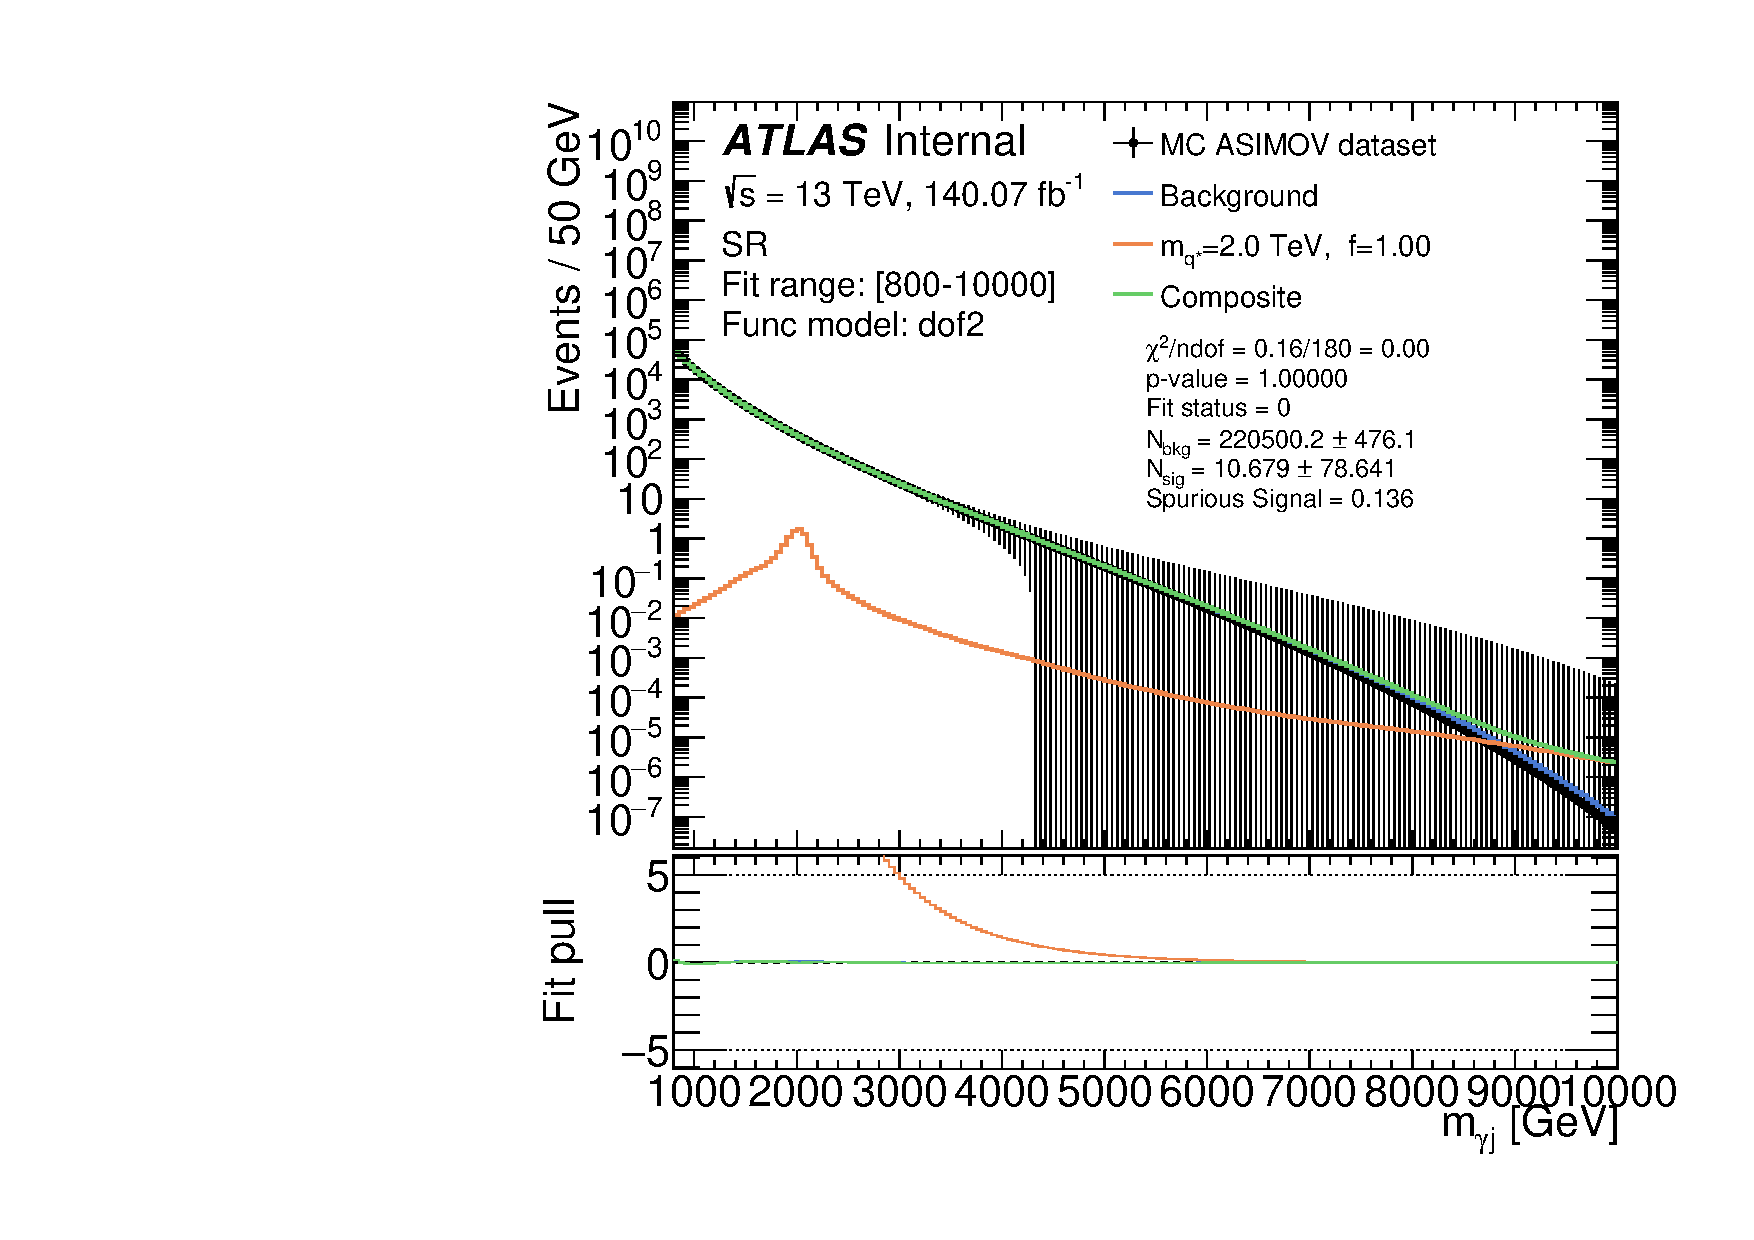
\includegraphics[width=\textwidth]{5_resonances/bkg/modeling/ss/asimov/fits/can__sigbkg_fit__asimov__photonjet_Pythia__SR__dof2__range_800-10000__qstar__qStar_f1p00_M2000}
        \caption{\(\mq = 2000~\gev\)}
    \end{subfigure}
    \hfill
    \begin{subfigure}[h]{0.49\linewidth}
        \centering
        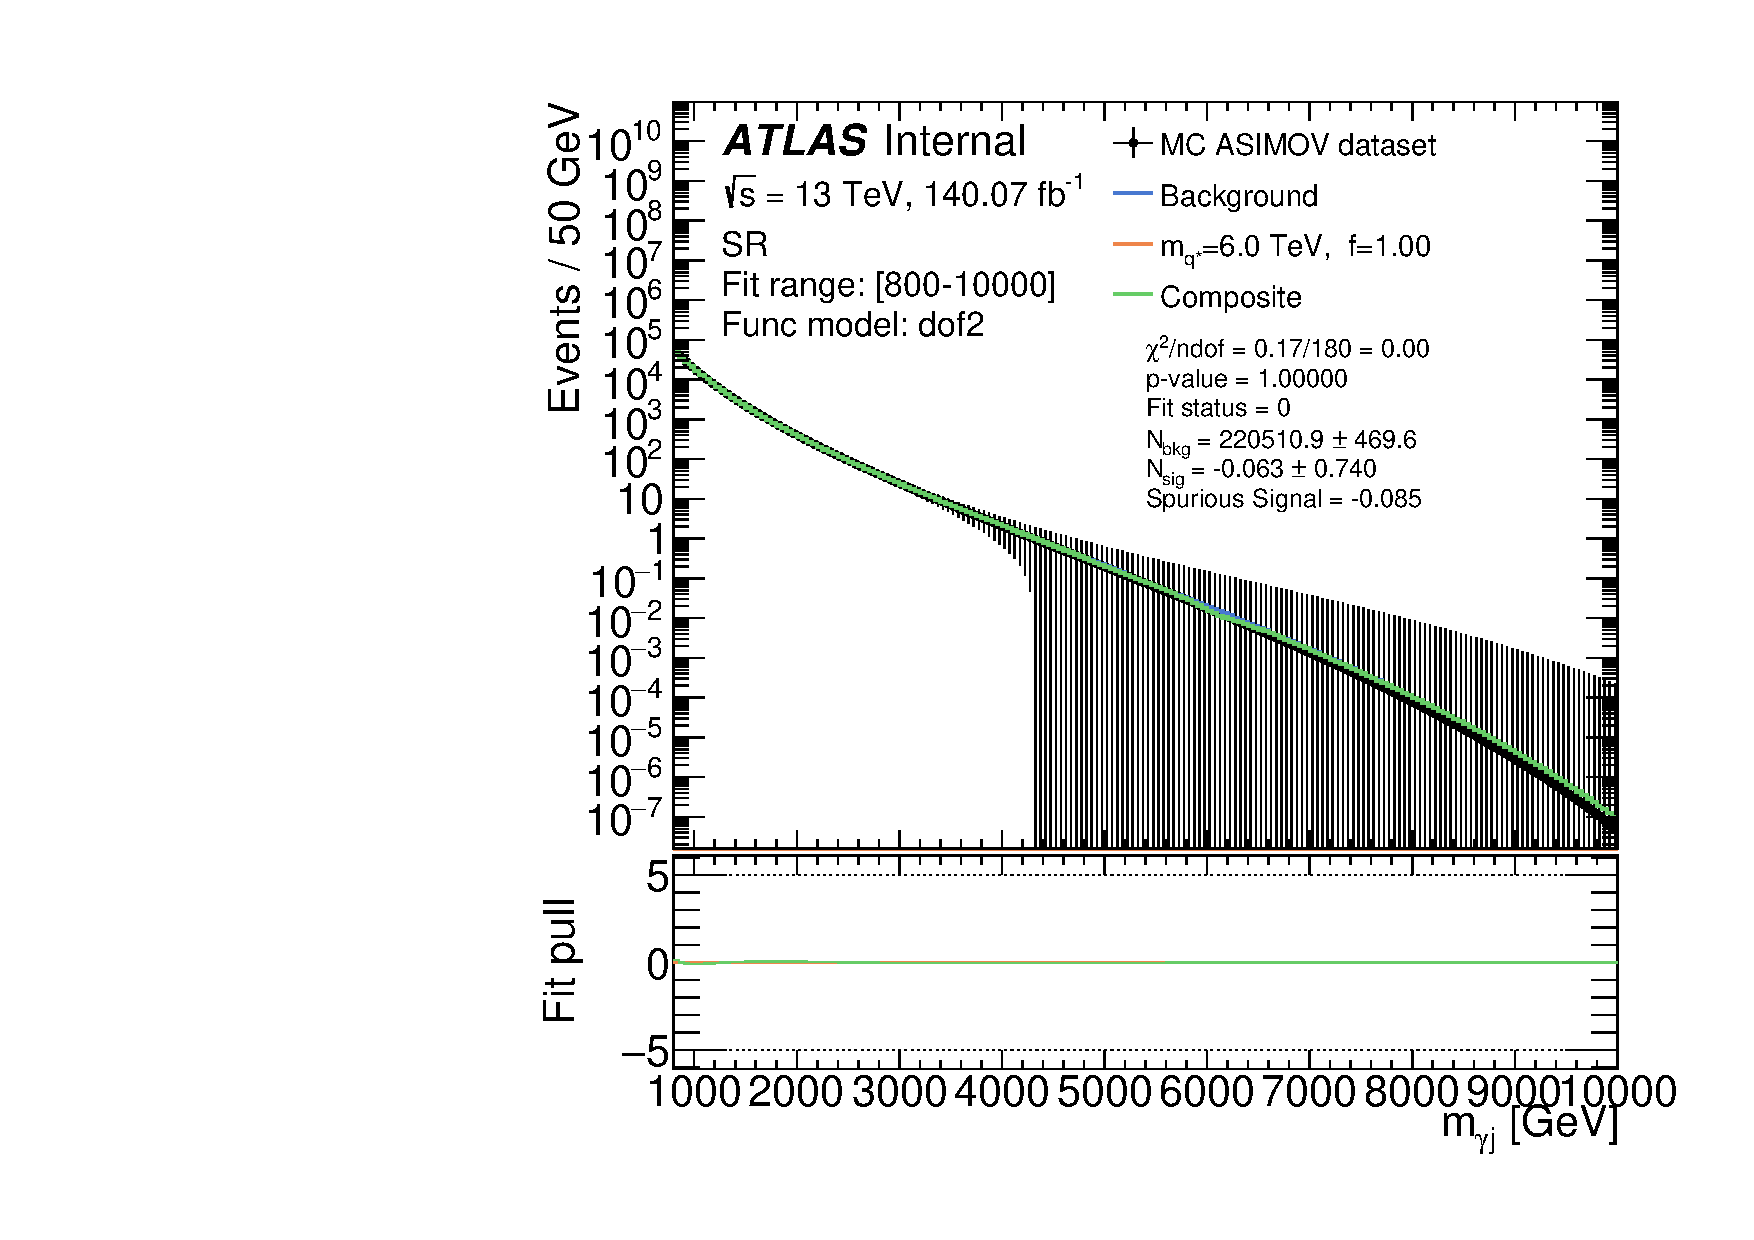
\includegraphics[width=\textwidth]{5_resonances/bkg/modeling/ss/asimov/fits/can__sigbkg_fit__asimov__photonjet_Pythia__SR__dof2__range_800-10000__qstar__qStar_f1p00_M6000}
        \caption{\(\mq = 6000~\gev\)}
    \end{subfigure}
    \caption{Ajuste \ac{SB} al fondo representado por una muestra Asimov para el cáclulo de la \ac{SSig}. El modelo de se\~nal se muestra con las líneas naranjas, la función que describe al fondo en este caso es la función \textit{dof2}, representada por la las líneas azules. Finalmente, la suma de las dos componentes se muestra con las líneas verdes. El panel inferior en ambas figuras muestras los residuos del ajuste, normalizados por la incerteza del histograma del fondo. También se muestran las normalizaciones resultantes del fondo y la se\~nal, junto con el valor de la \ac{SSig}.}
    \label{fig:bkg:modeling:sigbkg:sstest:sstest_asimov_examples}
\end{figure}

\begin{figure}[ht!]
    \centering
    \begin{subfigure}[h]{0.49\linewidth}
        \centering
        \includegraphics[width=\textwidth, page=24]{5_resonances/bkg/modeling/ss/toys/fits/can__sigbkg_fit__toys__photonjet_Pythia__SR__dof2__range_800-10000__qstar__qStar_f1p00_M2000}
    \end{subfigure}
    \hfill
    \begin{subfigure}[h]{0.49\linewidth}
        \centering
        \includegraphics[width=\textwidth, page=423]{5_resonances/bkg/modeling/ss/toys/fits/can__sigbkg_fit__toys__photonjet_Pythia__SR__dof2__range_800-10000__qstar__qStar_f1p00_M2000}
    \end{subfigure}
    \caption{ídem a la \Fig{\ref{fig:bkg:modeling:sigbkg:sstest:sstest_asimov_examples}} pero usando distribuciones de toys como muestra del fondo.}
    \label{fig:bkg:modeling:sigbkg:sstest:sstest_toys_examples}
\end{figure}

Los ajustes para los toys, por su parte, se muestran en la \Fig{\ref{fig:bkg:modeling:sigbkg:sstest:sstest_toys_examples}}, en las mismas condiciones que en la \Fig{\ref{fig:bkg:modeling:sigbkg:sstest:sstest_asimov_examples}}, sólo que para el modelo de \qstar con \(\mq=2000~\gev\). El resultado final de la \ac{SSig} para los toys se obtiene a partir de la distribución de \sspur de todos ajustes que hayan convergido. Como ejemplo, en la \Fig{\ref{fig:bkg:modeling:sigbkg:sstest:sstest_toys_distributions}} se muestran los ajustes en la región SR utilizando señales \qstar en el rango \(800-10000~\gev\) y con la función \textit{dof2}. En las figuras se muestran dos masas \qstar diferentes: \(2000\) y \(4000~\gev\). En el primer caso, el valor medio de la \sspur es mucho mayor que en el segundo, pero con una desviación estándar también mayor.

\begin{figure}[ht!]
    \centering
    \begin{subfigure}[h]{0.49\linewidth}
        \centering
        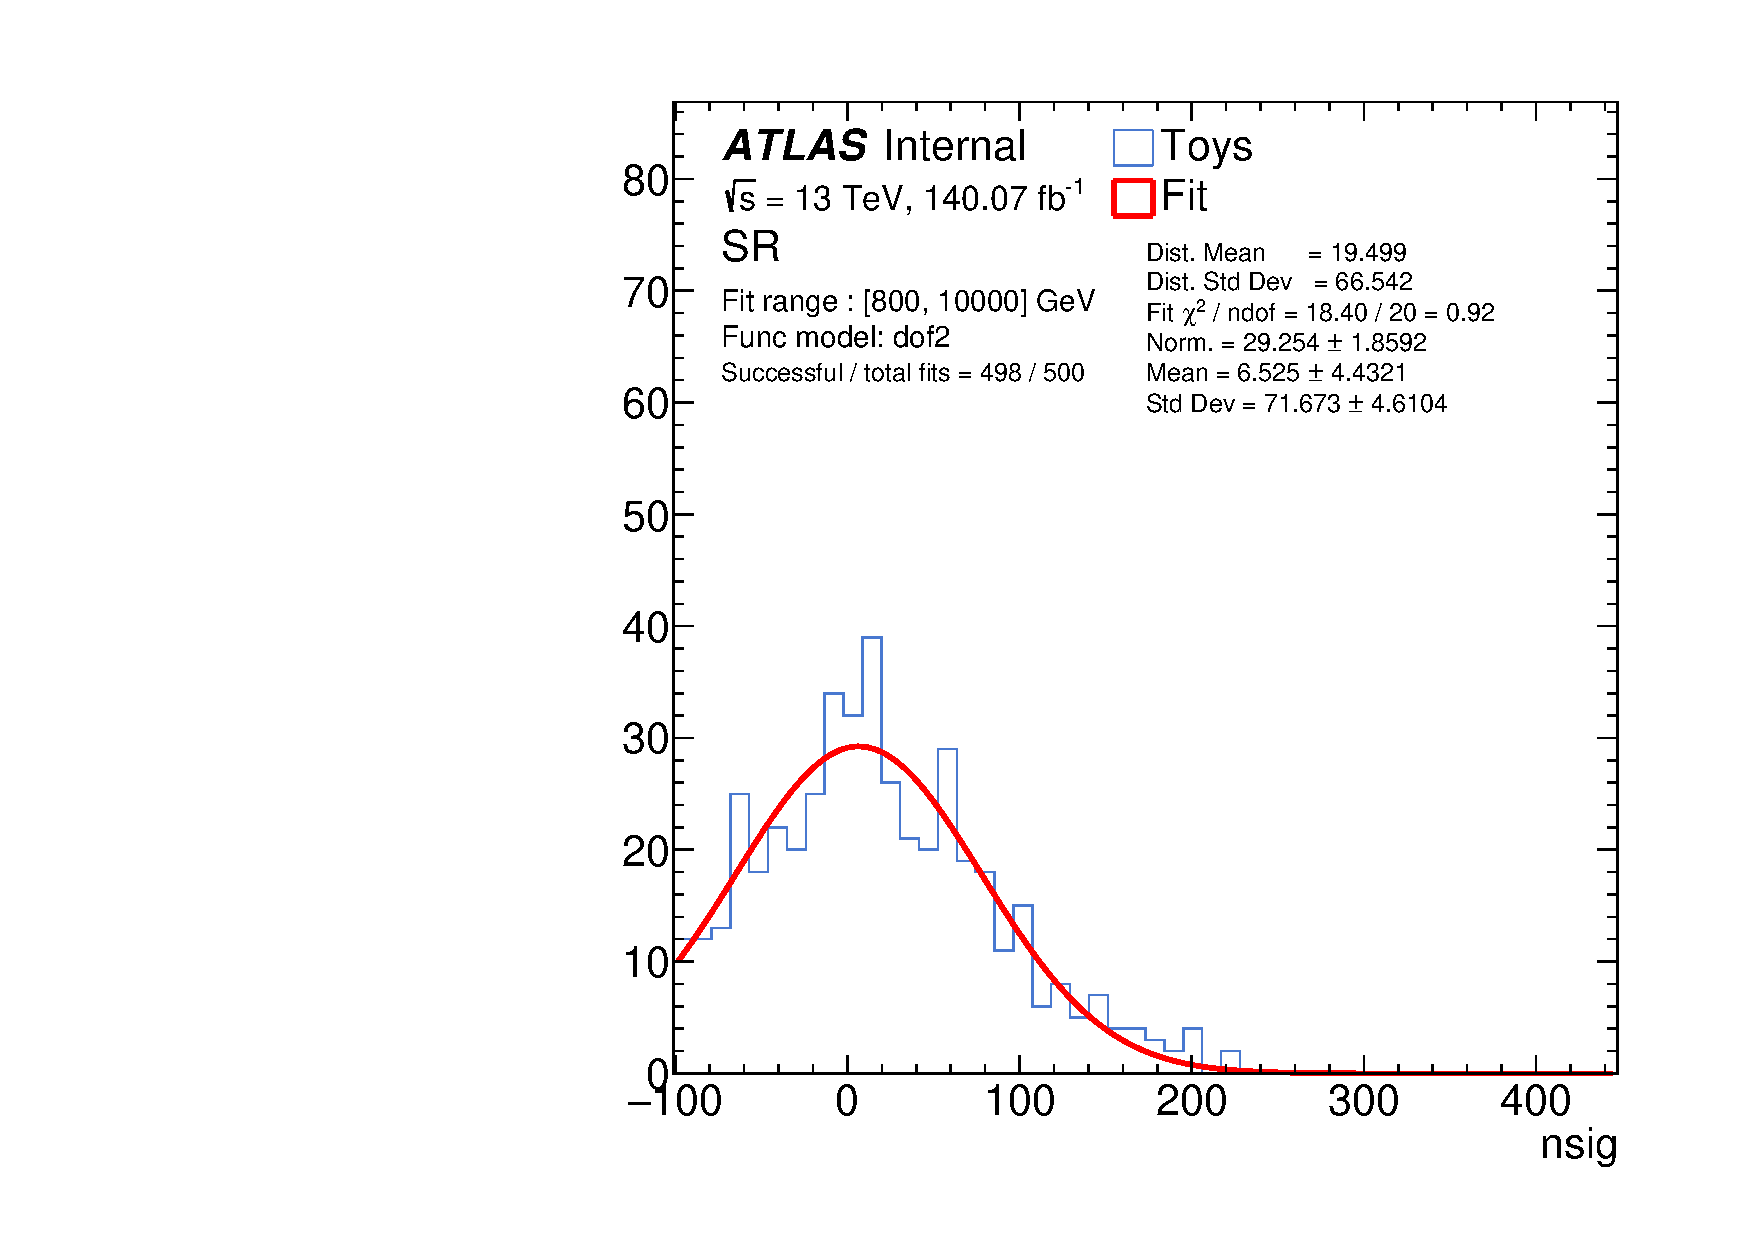
\includegraphics[width=\textwidth]{5_resonances/bkg/modeling/ss/toys/fits/can__photonjet_Pythia__SR__dof2__range_800_10000__qStar_f1p00_M2000__toys_nsig}
        \caption{\(\mq = 2000~\gev\)}
    \end{subfigure}
    \hfill
    \begin{subfigure}[h]{0.49\linewidth}
        \centering
        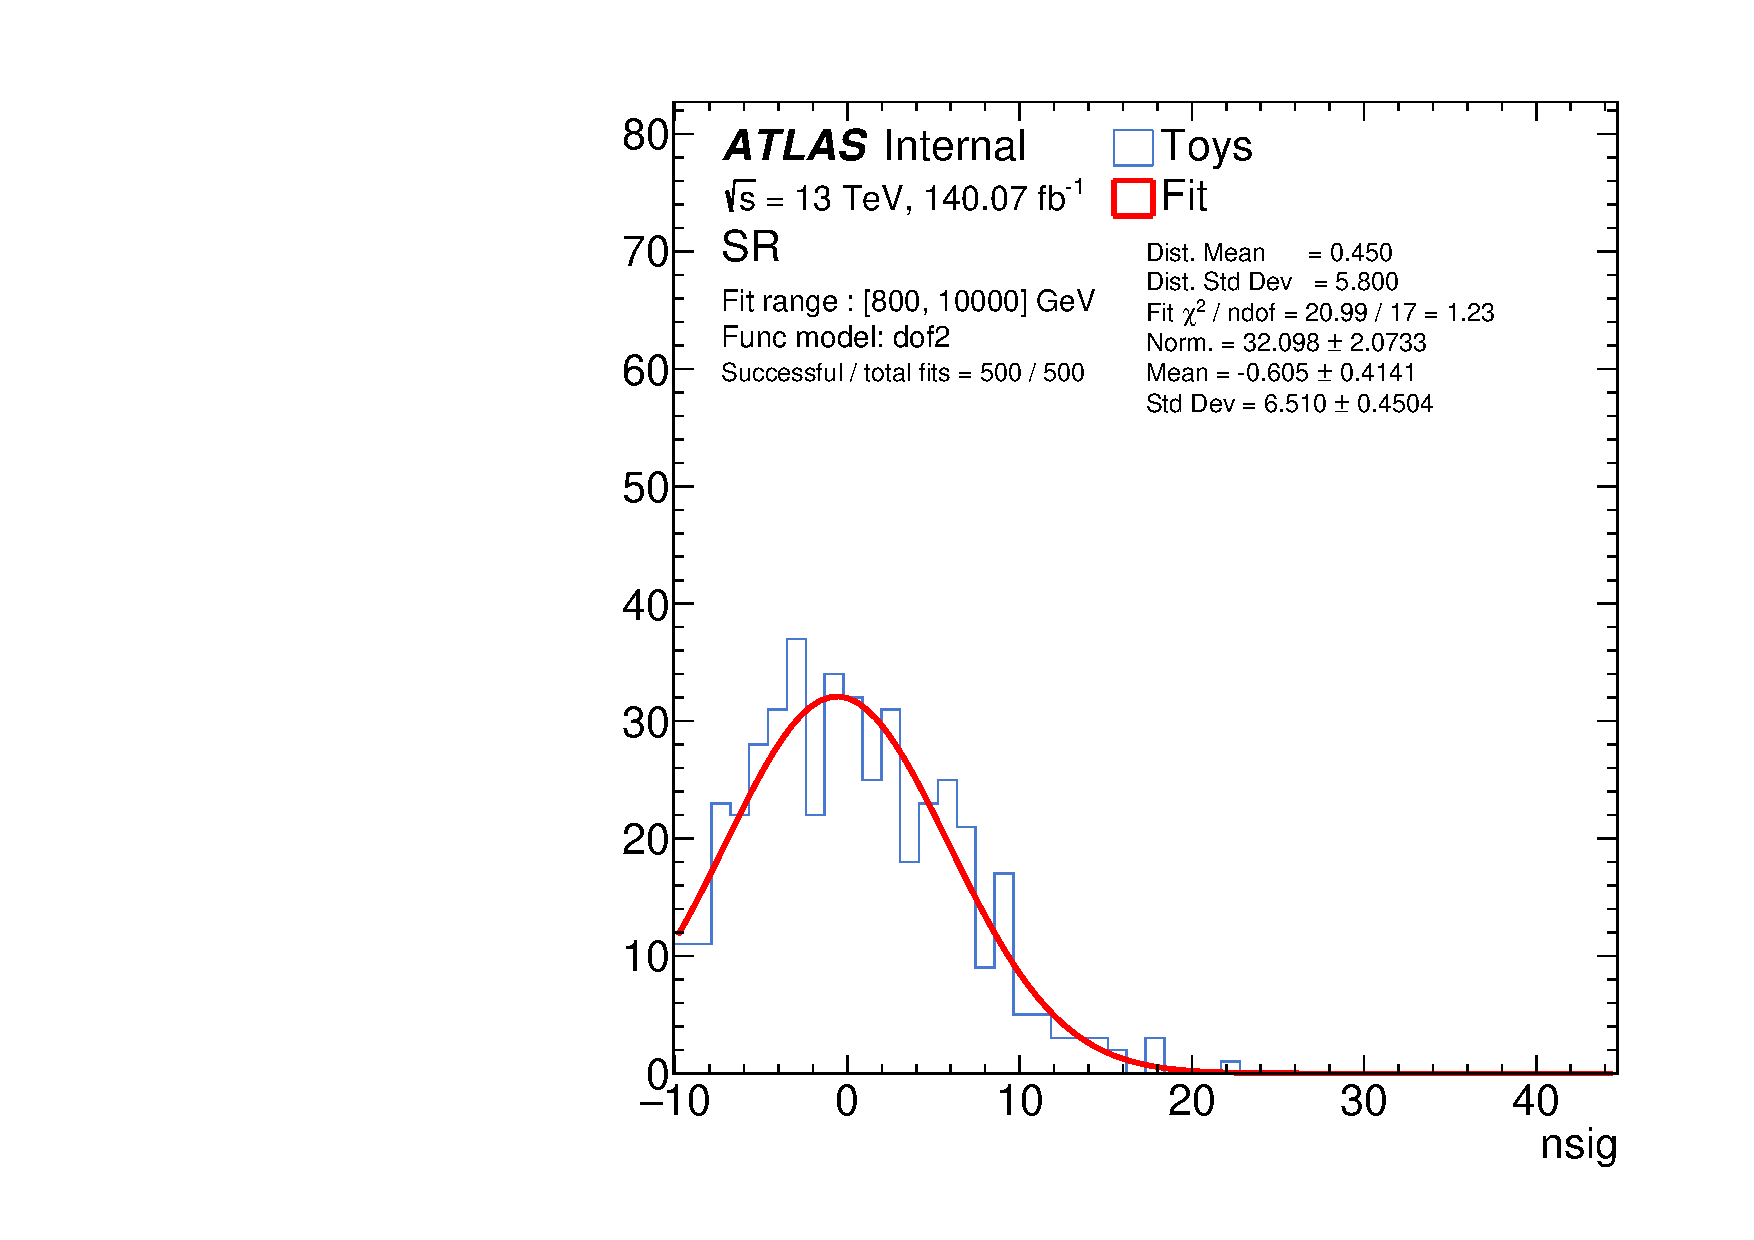
\includegraphics[width=\textwidth]{5_resonances/bkg/modeling/ss/toys/fits/can__photonjet_Pythia__SR__dof2__range_800_10000__qStar_f1p00_M4000__toys_nsig}
        \caption{\(\mq = 4000~\gev\)}
    \end{subfigure}
    \caption{Distribución de \ac{SSig} (histograma azul) en la región SR, con un ajuste Gaussian. El valor final de la \ac{SSig} se obtiene directamente de la distribución, no del ajuste. La función utilizada para realizar el ajuste es el \textit{dof2} y el ajuste se realiza en el rango de \([800, 1000]~\gev\). La se\~nal utilizada corresponde a \qstar con \(f=1\).}
    \label{fig:bkg:modeling:sigbkg:sstest:sstest_toys_distributions}
\end{figure}


En general, para que un modelo pase el test de \ac{SSig}, el valor \sspur tiene que estar dentro de los límites aceptables de:
\begin{equation}
    \label{eq:bkg:modeling:sigbkg:sstest:condition}
    |\sspur| < 0.5 \sigma_{\text{fit}}
\end{equation}
y sólo después puede utilizarse para estudios posteriores. En los dos casos mostrados en la \Fig{\ref{fig:bkg:modeling:sigbkg:sstest:sstest_toys_distributions}}, se pasa el test, donde los coeficientes \(\sspur / \sigma_{\text{fit}}\) son \(19.5 / 66.5 = 0.29\) y \(0.45 / 5.80 = 0.07\) para las masas \(\mq = 2000\) y \(\mq = 4000~\gev\), respectivamente.
% El objetivo principal de estos tests es encontrar un grupo de funciones apropiadas para ser utilizadas, así como el rango de ajuste óptimo para estos modelos funcionales. Se consideran diferentes límites inferiores y superiores para los rangos de ajuste dependiendo de la región de la señal que se esté estudiando.

La \Fig{\ref{fig:bkg_modeling:sstest_results_asimov_SR}} muestra los resultados de la \ac{SSig} para los tres modelos de se\~nal estudiados en la región SR, donde el fondo está representado por las muestras Asimov. En cada figura, se comparan las diferentes funciones para un rango fijo de ajuste, siendo este el rango en el que la \ac{SSig} es mínima. De forma similar, los resultados utilizando los toys se encuentran en la \Fig{\ref{fig:bkg_modeling:sstest_results_toys_SR}}. Estas figuras muestran en el panel superior el valor de la \sspur para cada masa. En el panel inferior, por su parte, muestra el cociente \(\sspur / \sigma_{\text{fit}}\), el cual se espera que se cumpla la \Eqn{\ref{eq:bkg:modeling:sigbkg:sstest:condition}} para cada masa de se\~nal.

De la comparación de la \Fig{\ref{fig:bkg_modeling:sstest_results_asimov_SR}} (Asimov) y \Fig{\ref{fig:bkg_modeling:sstest_results_toys_SR}} (toys) se puede ver que en el caso de los toys, los tests de \ac{SSig} se han realizado con señales con masas hasta \(5000~\gev\). La razón detrás de esto es la ausencia de eventos en las distribuciones \myj para \(\myj \gtrsim 5.5~\tev\).
% (como se vió en la \Sect{\ref{subsubsec:bkg:modeling:preparation:toys}}), por lo que un ajuste de \ac{SB} a cero eventos carece de significado físico.


\begin{figure}[ht!]
    \centering
    \begin{subfigure}[h]{0.32\linewidth}
        \centering
        \includegraphics[width=\textwidth]{5_resonances/bkg/modeling/ss/asimov/results/SR/gaus/width0p02/plots/can__SS__photonjet_Pythia__gaus__SR__width0p02__range_1200_8000}
        \caption{Gaussiana con \(\sigma_G / \mG = 0.02\).}
    \end{subfigure}
    \hfill
    \begin{subfigure}[h]{0.32\linewidth}
        \centering
        \includegraphics[width=\textwidth]{5_resonances/bkg/modeling/ss/asimov/results/SR/qstar/q_1p00/plots/can__SS__photonjet_Pythia__qstar__SR__q_1p00__range_1000_8000}
        \caption{\qstar.}
    \end{subfigure}
    \begin{subfigure}[h]{0.32\linewidth}
        \centering
        \includegraphics[width=\textwidth]{5_resonances/bkg/modeling/ss/asimov/results/SR/QBH/n1/plots/can__SS__photonjet_Pythia__QBH__SR__n1__range_1000_8000}
        \caption{\ac{QBH} con \(n=1\).}
    \end{subfigure}\\
    \caption{Resultados de los tests de \ac{SSig} en la región SR donde el fondo está representado por una muestra Asimov. Las diferentes figuras corresponden a los 3 modelos de se\~nal considerados en esta tesis. Para cada caso, se muestran los resultados de la \ac{SSig} en el rango de ajuste que da la mínima \ac{SSig}, y las distintas funciones utilizadas están representadas por los puntos de diferentes colores.}
    \label{fig:bkg_modeling:sstest_results_asimov_SR}
\end{figure}


\begin{figure}[ht!]
    \centering
    \begin{subfigure}[h]{0.32\linewidth}
        \centering
        \includegraphics[width=\textwidth]{5_resonances/bkg/modeling/ss/toys/results/SR/gaus/width0p02/plots/can__SS__photonjet_Pythia__gaus__SR__width0p02__range_1200_8000}
        \caption{Gaussiana con \(\sigma_G / \mG = 0.02\).}
    \end{subfigure}
    \hfill
    \begin{subfigure}[h]{0.32\linewidth}
        \centering
        \includegraphics[width=\textwidth]{5_resonances/bkg/modeling/ss/toys/results/SR/qstar/q_1p00/plots/can__SS__photonjet_Pythia__qstar__SR__q_1p00__range_1000_8000}
        \caption{\qstar.}
    \end{subfigure}
    \begin{subfigure}[h]{0.32\linewidth}
        \centering
        \includegraphics[width=\textwidth]{5_resonances/bkg/modeling/ss/toys/results/SR/QBH/n1/plots/can__SS__photonjet_Pythia__QBH__SR__n1__range_1000_8000}
        \caption{\ac{QBH} con \(n=1\).}
    \end{subfigure}\\
    \caption{ídem a la \Fig{\ref{fig:bkg_modeling:sstest_results_asimov_SR}} pero los resultados provienen de utilizar toys como el fondo.}
    \label{fig:bkg_modeling:sstest_results_toys_SR}
\end{figure}


Debido a que se cuenta con dos metodologías (muestras de toys y Asimov) para calcular el test de \ac{SSig}, los resultados de ambos se combinan dando preferencia a los toys, ya que se calculan de forma más robusta. La combinación se realiza del siguiente modo:
\begin{enumerate}
    \item Se utilizan los resultados de \ac{SSig} procedentes de toys hasta el punto de masa en el que se espera que haya una cantidad considerable de eventos de fondo. El punto de masa máximo considerado para todas las regiones dominadas por \ljets (\bjets y \cjets) es \(<5~\tev\) (\(<4~\tev\)). Por tanto, los resultados de \acp{SSig} utilizando toys sólo contribuyen hasta \(\sim 5~\tev\).
    \item Los resultados de \ac{SSig} utilizando las muestras de Asimov se utilizan para el resto del rango de masas, por lo que sólo contribuyen en el rango \(> 5~\tev\).
\end{enumerate}
La \ac{SSig}, o sesgo de ajuste, se utiliza en los ajustes finales a los datos como una de las incertezas sistemáticas asociadas al modelado del fondo, por lo que se desea que esta incerteza sea lo más pequeña posible. Para cada región de señal y modelo de señal, después de realizar la combinación anteriormente mencionada, se crea un ranking de los rangos de ajuste y modelos funcionales, basado en la media absoluta de \ac{SSig}. Esta cantidad indica qué combinación de rango de ajuste y modelo funcional proporciona la menor \ac{SSig} en promedio para cada punto de masa, dando la misma importancia a cada masa.

































\subsubsection{Tests de \acl{SI}}
\label{subsubsec:bkg:modeling:sigbkg:sitest}

El test de \acf{SI} comprueba la capacidad de una estrategia de ajuste de determinar correctamente la cantidad de señal presente en un conjunto de datos. Se realiza de forma similar al test de \ac{SSig}, con la diferencia de que se inyecta una señal de la hipótesis esperada con cierta amplitud sobre los pseudodatos o toys de \ac{BO}. Mientras que la definición de \sspur para los tests de \ac{SSig} era simplemente el número de eventos de señal extraídos, mostrado por la \Eqn{\ref{eq:bkg:modeling:sigbkg:sstest:sspur_definition_sstest}}, en estos tests se generaliza de tal manera que \sspur es ahora la diferencia entre las señales extraídas y las inyectadas:
\begin{equation}
    \label{eq:bkg:modeling:sigbkg:sitest:sspur_definition}
    \sspur = 
    \begin{cases}
        N_{\text{fit}} - N_{\text{inj}} & \qif \text{Asimov dataset},\\
        \expval{N_{\text{fit}} - N_{\text{inj}}}_{\text{toys}} & \qif \text{Toys dataset}.
    \end{cases}
\end{equation}

La amplitud de la inyección se denota en unidades de \(\sqrt{B}\), que tiene en cuenta la raíz cuadrada del número de eventos de fondo en el rango \ac{FWHM} de la señal en cuestión, corregida por el número de eventos de señal en dicho rango:
\begin{equation*}
    \sqrt{B} \equiv \frac{
        \displaystyle
        \sqrt{\sum_{\text{bins in FWHM}} b_i}
        }{
        \displaystyle
        \sum_{\text{bins in FWHM}} s_i 
    }
\end{equation*}
La inclusión de esta corrección tiene por objetivo que las amplitudes reportadas en unidades de \(\sqrt{B}\) correspondan siempre a relaciones \(S / \sqrt{B}\).

Los tests de de \ac{SI}, se realizan con 300 toys por hipótesis de señal, región de señal y amplitud de inyección, en los mismos rangos que en los tests de \ac{SSig}, y utilizando diferentes modelos funcionales. El criterio recomendado para pasar los tests de \ac{SI} es \(|\sspur| < 0.5 N_{\text{inj}}\). En la \Fig{\ref{fig:bkg:modeling:sigbkg:sitest:siginj_qstar}}, se muestran ejemplos del test para el modelo de señal \ac{EQ}. En los paneles superiores de las figuras se muestra, en función de \(N_{\text{sig}}^{\text{inj}} / \sqrt{B}\), la señal extraída en el rango \ac{FWHM} \(N_{\text{sig}}^{\text{fit}} / \sqrt{B}\) para diferentes masas. Los paneles inferiores de los gráficos muestran la \sspur calculada como en la \Eqn{\ref{eq:bkg:modeling:sigbkg:sitest:sspur_definition}}, dividida por la amplitud de la señal inyectada \(N_{\text{inj}}\). En todos los casos, se supera el test de \ac{SI}, ya que la relación es \(<0.5\). Además, se observa que los resultados muestran una linealidad muy buena. Los resultados de los demás modelos de señal se muestran en \App{\ref{app:si_results}}, donde se observa una buena linealidad en todos los casos.
% \fixme{revise definition of ratio. Should it be with the uncertainty, or with the injecected signal?}

\begin{figure}[ht!]
    \centering
    \begin{subfigure}[h]{0.49\linewidth}
        \centering
        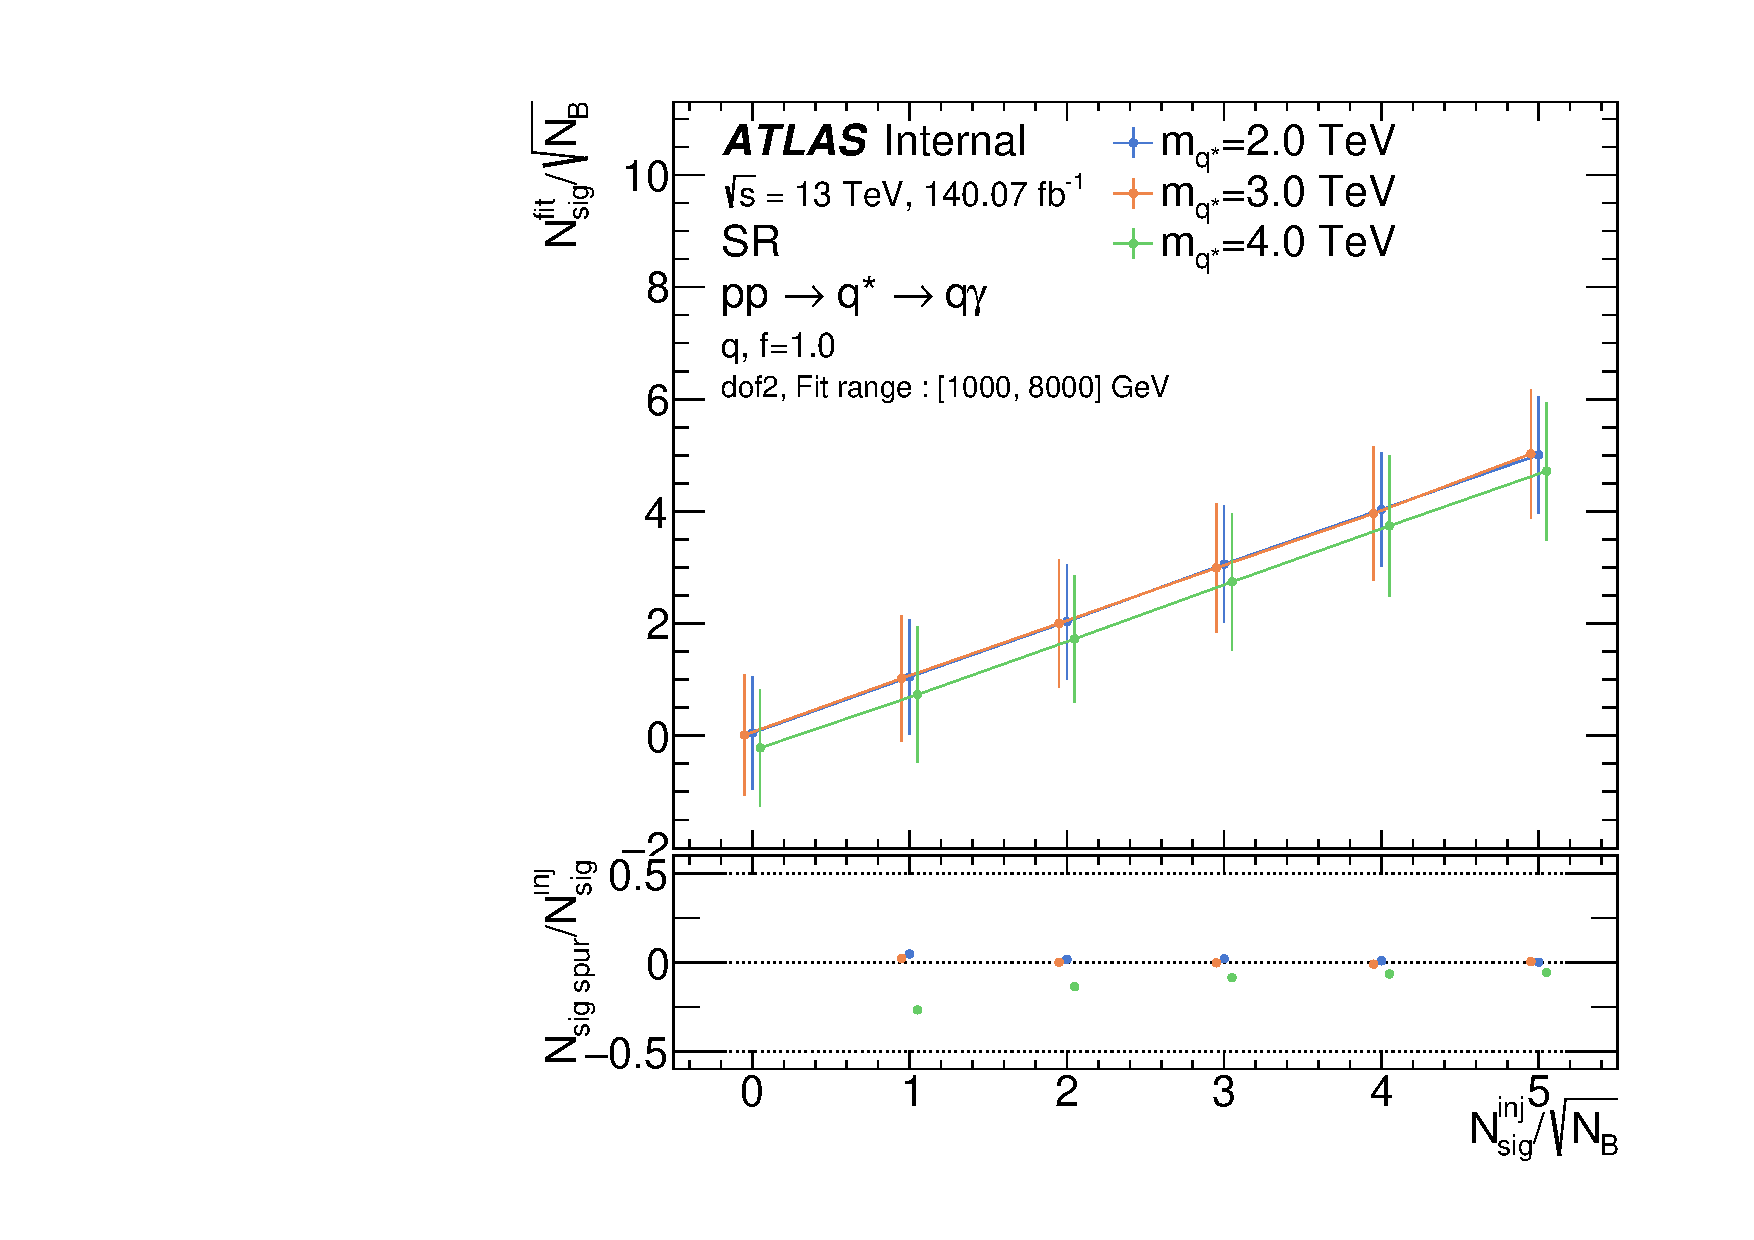
\includegraphics[width=\textwidth]{5_resonances/bkg/modeling/si/toys/SR/qstar/q_1p00/dof2__range_1000_8000/plots/can__SigInj__photonjet_Pythia_jfakeisosmooth__qstar__SR__q_1p00__dof2__range_1000_8000}
        \caption{SR.}
    \end{subfigure}
    \hfill
    \begin{subfigure}[h]{0.49\linewidth}
        \centering
        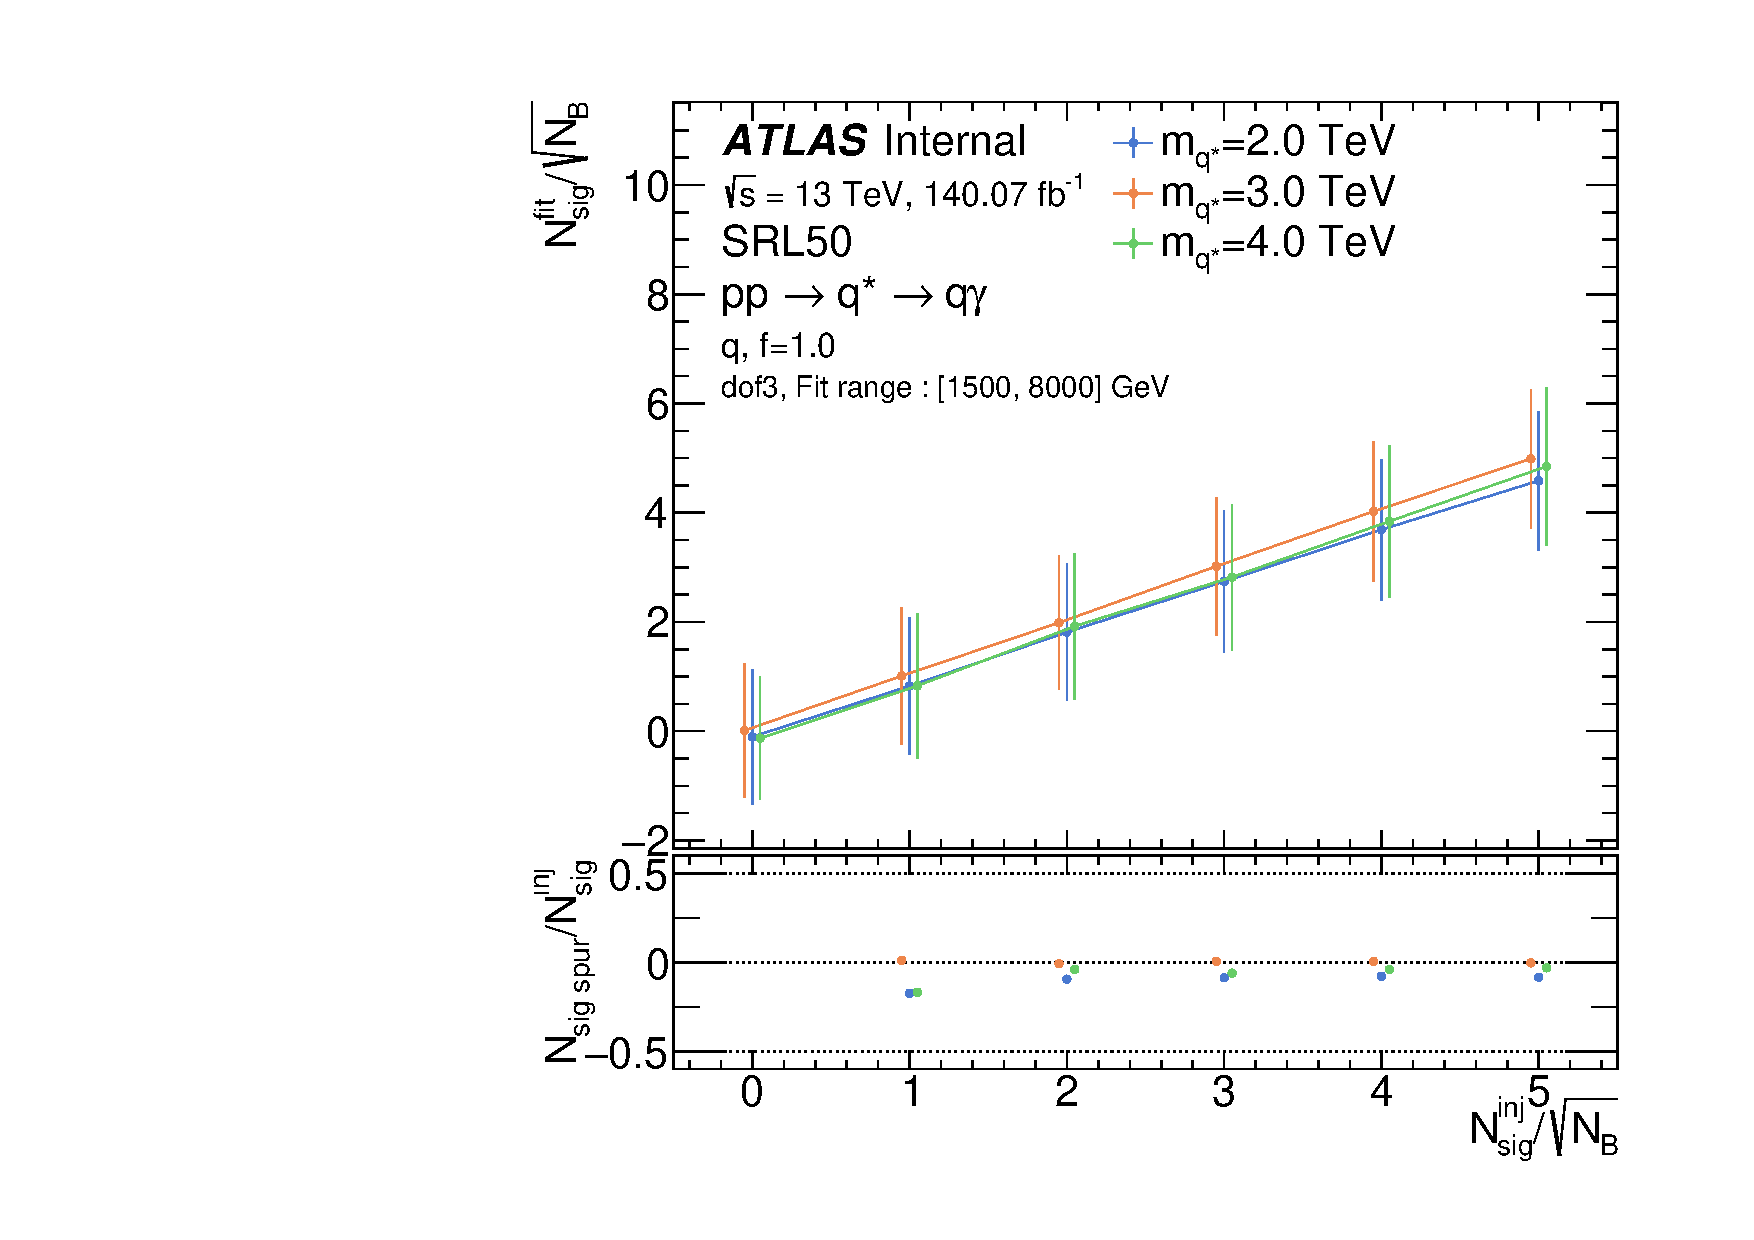
\includegraphics[width=\textwidth]{5_resonances/bkg/modeling/si/toys/SRL50/qstar/q_1p00/dof3__range_1500_8000/plots/can__SigInj__photonjet_Pythia_jfakeisosmooth__qstar__SRL50__q_1p00__dof3__range_1500_8000}
        \caption{SRL.}
    \end{subfigure}\\
    \begin{subfigure}[h]{0.49\linewidth}
        \centering
        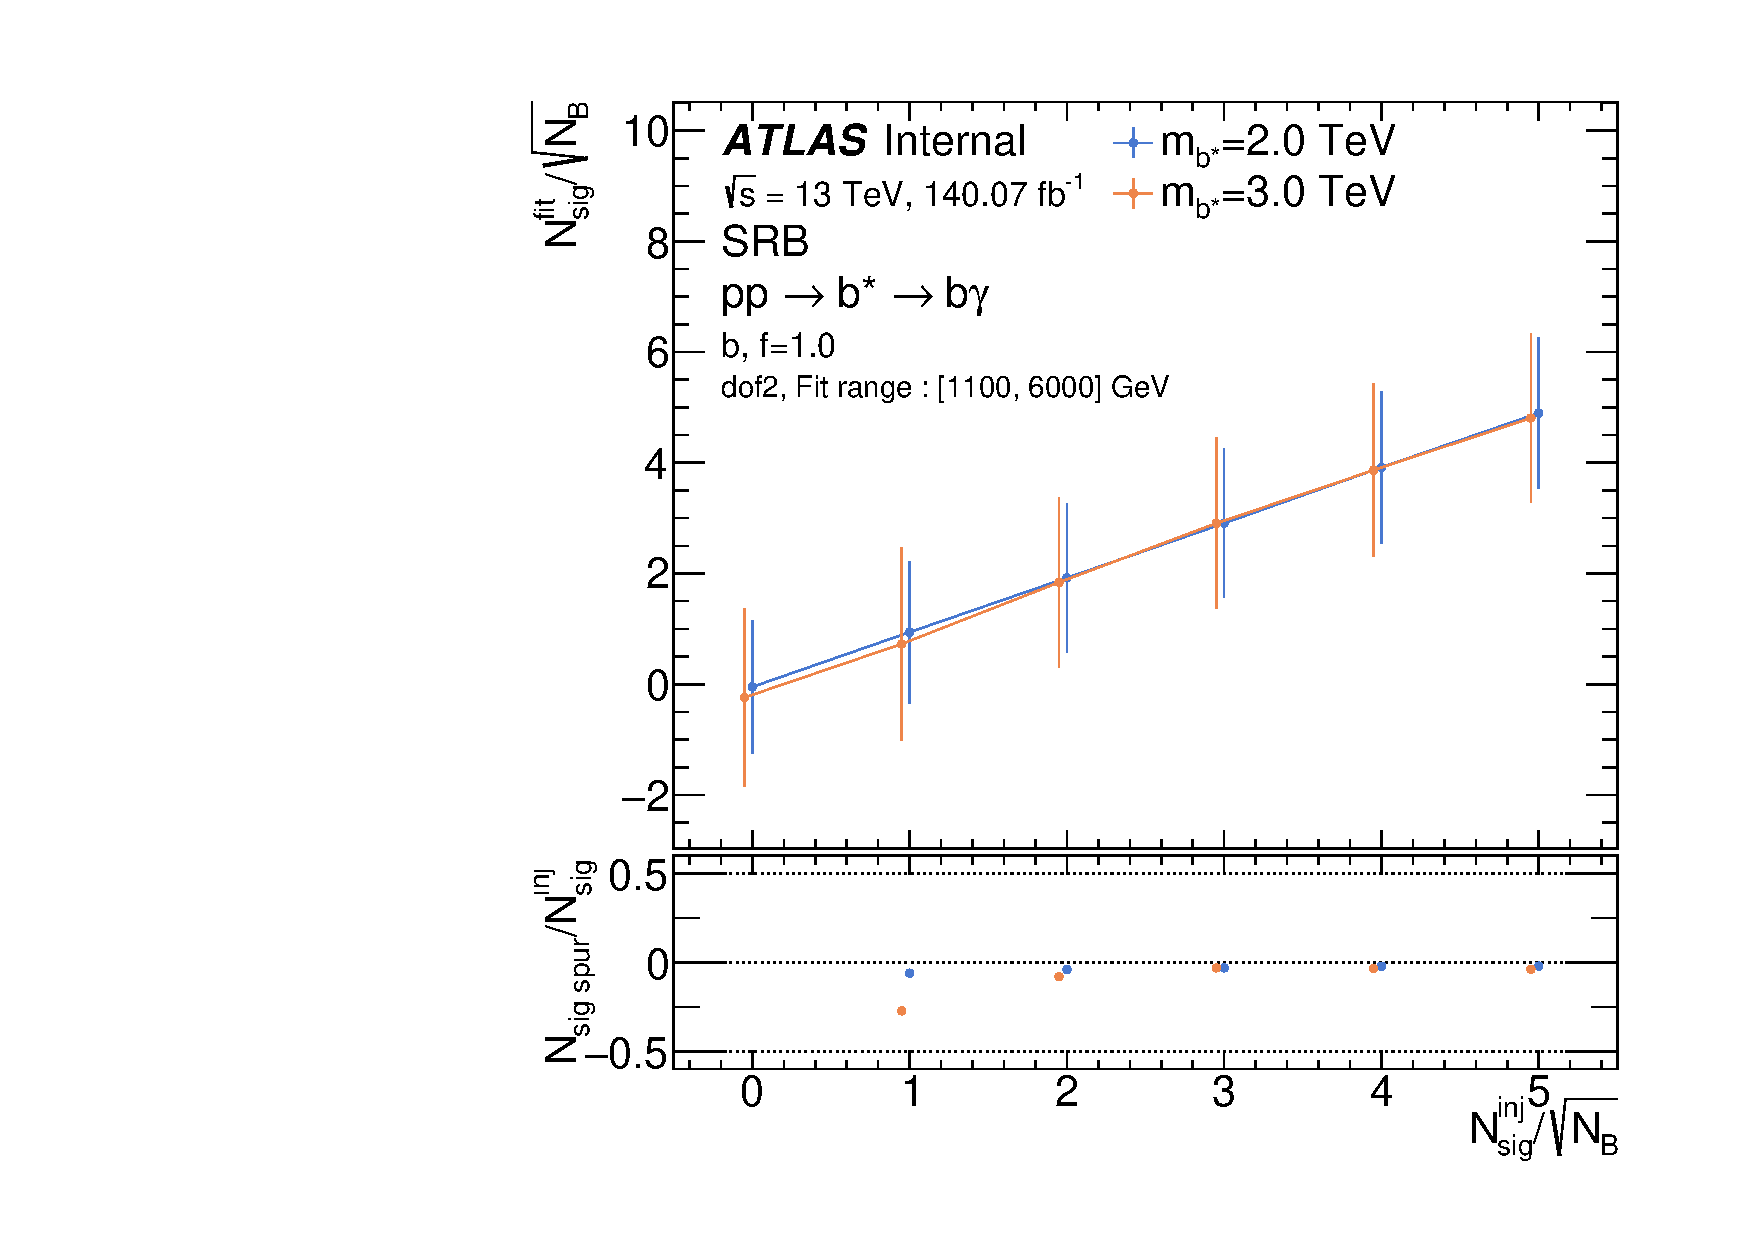
\includegraphics[width=\textwidth]{5_resonances/bkg/modeling/si/toys/SRB/qstar/b_1p00/dof2__range_1100_6000/plots/can__SigInj__photonjet_Pythia_jfakeisosmooth__qstar__SRB__b_1p00__dof2__range_1100_6000}
        \caption{SRB.}
    \end{subfigure}
    \hfill
    \begin{subfigure}[h]{0.49\linewidth}
        \centering
        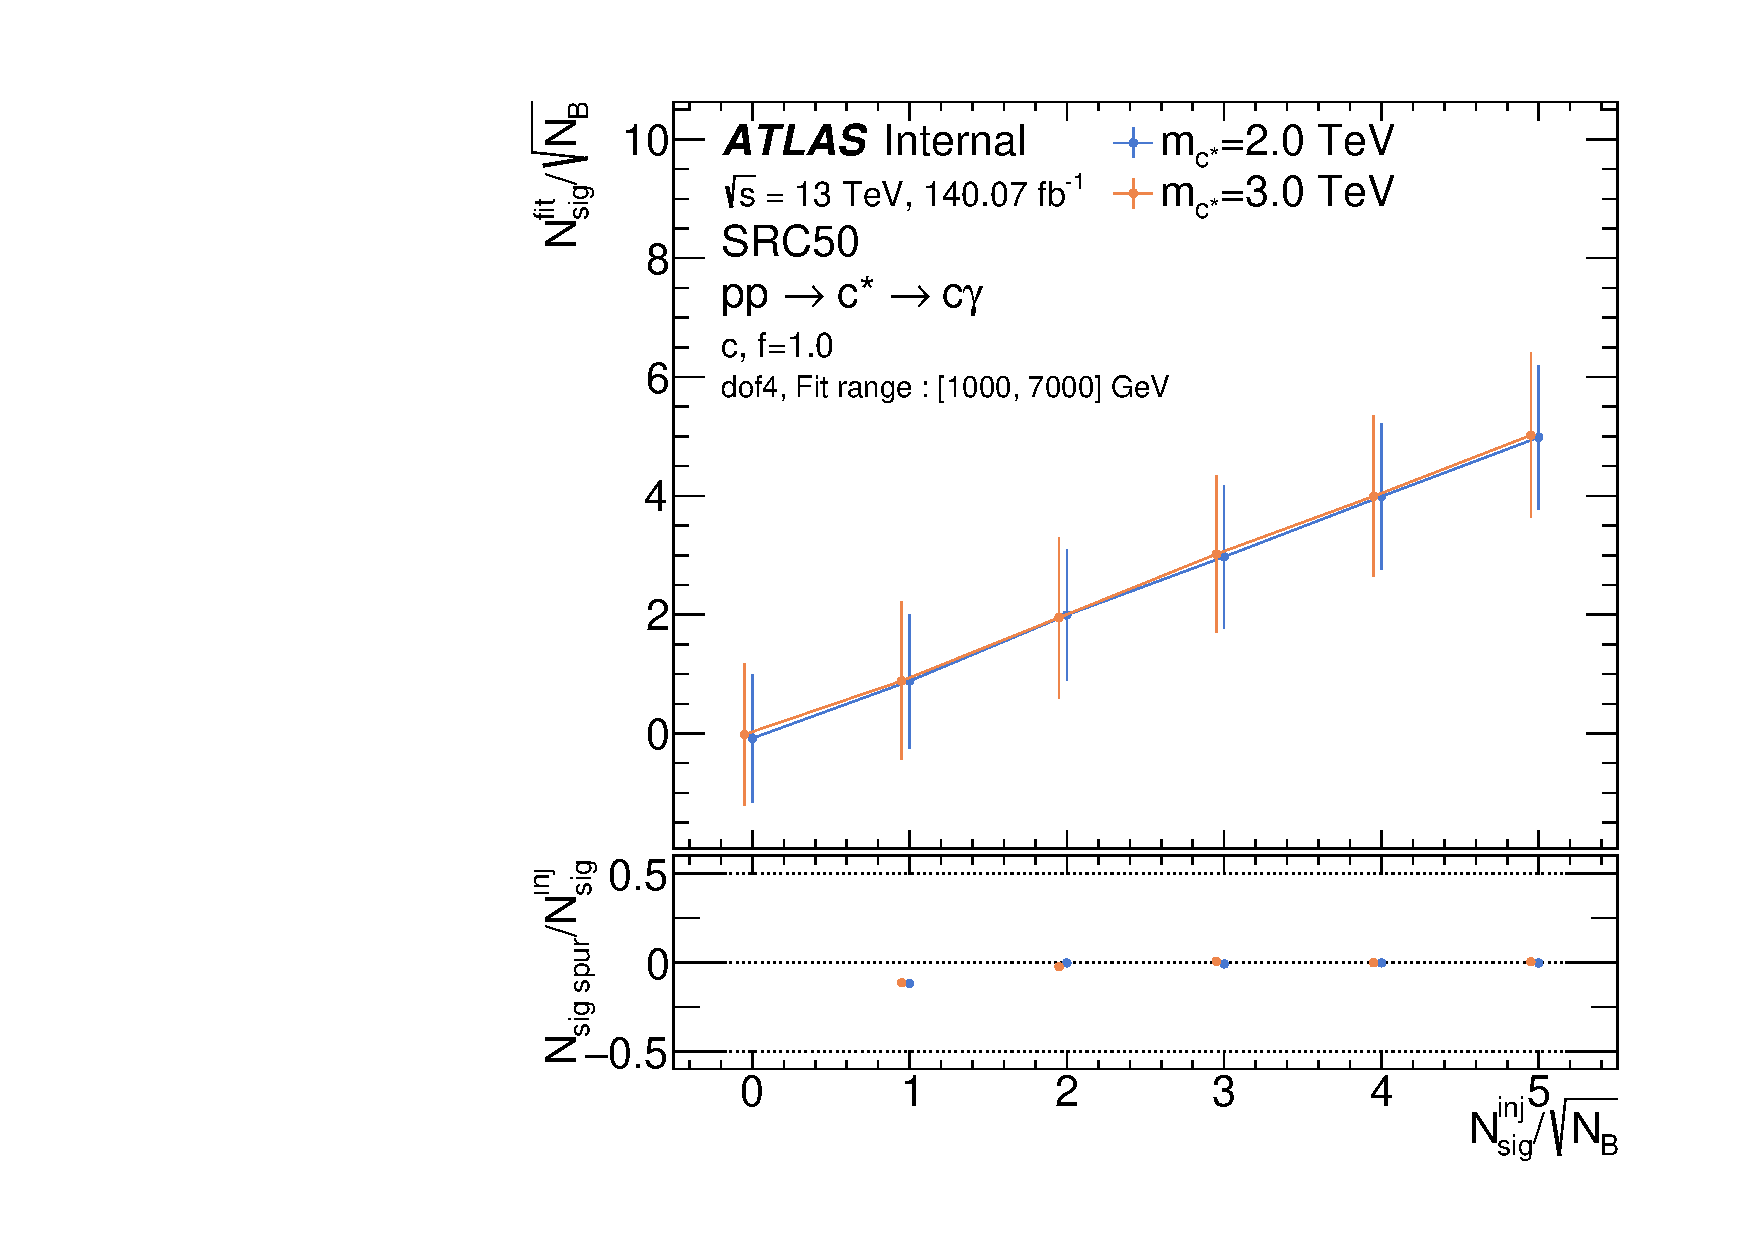
\includegraphics[width=\textwidth]{5_resonances/bkg/modeling/si/toys/SRC50/qstar/c_1p00/dof4__range_1000_7000/plots/can__SigInj__photonjet_Pythia_jfakeisosmooth__qstar__SRC50__c_1p00__dof4__range_1000_7000}
        \caption{SRC.}
    \end{subfigure}\\
    \caption{Resultados de los test de \ac{SI} utilizando el modelo teórico de \ac{EQ} en las regiones SR, SRL, SRB and SRC, respectively. En cada caso, el rango del fit y la forma funcional que dan la menor \ac{SSig} son utilizados. Cada se\~nal, correspondiendo a diferentes masas, se muestra con un color diferente. El eje-\(x\) muestra la amplitud de la se\~nal inyectada en unidades de \(\sqrt{N_B}\), mientras que el eje\(y\) representa la se\~nal extraída en unidades de \(\sqrt{N_B}\).}
    \label{fig:bkg:modeling:sigbkg:sitest:siginj_qstar}
\end{figure}































\subsubsection{Tests-\(F\)}
\label{subsubsec:bkg:modeling:preparation:ftest}

Una vez establecidos el rango de ajuste óptimo y la clasificación de una función en virtud de los tests de \ac{SSig}, el último test estadístico utilizado para determinar la función para modelar el fondo se conoce como test-\(F\). El test compara los ajustes realizados con una función \(a\) con parámetros \(p_a = n\) con otra función \(b\) que tiene parámetros \(p_b = n+1\). Para el test-\(F\), el modelo \(a\) es un subconjunto del modelo \(b\). En este test, se calcula un estadístico de prueba \(F\) a partir de los valores \chisq resultantes:
\begin{equation}
    \label{eq:bkg:modeling:preparation:ftest:ftest}
    F = \frac{
        \displaystyle
        \frac{\chisq_a - \chisq_b}{p_b - p_a}
    }{
        \displaystyle
        \frac{\chisq_b}{N - p_b}
    },
\end{equation}
donde \(N\) es el número total de bines de la muestra. De la ecuación anterior, se puede notar que \(F \ra 0\), implica \(\chisq_a - \chisq_b \ra 0\), indicando que los ajustes realizados por ambas funciones arrojan resultados similares. Por el contrario, valores altos de \(|F|\) significan que existen diferencias entre las dos funciones, la cual una se ajusta mejor a los datos.
Cuando \(F\) toma valores grandes positivos, indica que la función \(a\) no logra ajustar tan bien los datos como lo hace la función más compleja \(b\).
% Es importante notar el caso en el que \(F < 0\), ya que indica que la función más simple logra describir los datos mejor que la función más compleja. Esto se puede dar cuando al agregar un parámetro más a la función resulta en una 


% que el modelo con \(n\) parámetros debe descartarse, mientras que en los casos en los que \(F \to 0\) (\(\chisq_a - \chisq_b \to 0\)), la diferencia entre los modelos no es significativa, lo que lleva a seleccionar el modelo con la menor cantidad de parámetros, es decir, el modelo \(a\) con \(n\) parámetros.

Para discernir entre estos casos, se define la hipótesis nula, \(H_0\), como aquella en la que el modelo \(b\) no proporciona una mejor diferencia significativa en comparación con el modelo \(a\) (pequeño \(F\)), y en esta situación, \(F\) tendrá una distribución \(F\) con \((p_b - p_a, N - p_b)\) \ac{dof}. La hipótesis nula se rechaza si el valor \(F\) es superior a un valor crítico, normalmente fijado en el que da lugar a un \(p\left(F(p_b-p_a, N-p_b)\right)<0.05\). En resumen, si el \pval de la comparación de los modelos \(a\) y \(b\) es \(>0.05\), no se rechaza la hipótesis nula y los dos modelos se consideran similares, mientras que los valores p \(<0.05\) significan que hay pruebas en contra de la hipótesis nula y se rechaza el modelo más simple \(a\).
Para el estudio de selección de la función de mejor ajuste, el modelo \(a\) es la función nominal con \textit{dofn} y el modelo \(b\) es la función alternativa \textit{dof(n+1)}.

Los ajustes se realizan con toys extraídos del ajuste \textit{dof7} de la distribución de \ac{BO} de \ac{MC}. Los rangos de ajuste seleccionados para estos estudios son los decididos a partir del test de \ac{SSig} anterior. Los modelos \(a\) y \(b\) se ajustan al mismo toy, y se comparan sólo si ambos ajustes convergen. Para cada uno de los toys, se calcula el valor \(F\) según la \Eqn{\ref{eq:bkg:modeling:preparation:ftest:ftest}}, y finalmente, el valor \(p\).



\begin{figure}[ht!]
    \centering
    \begin{subfigure}[h]{0.49\linewidth}
        \centering
        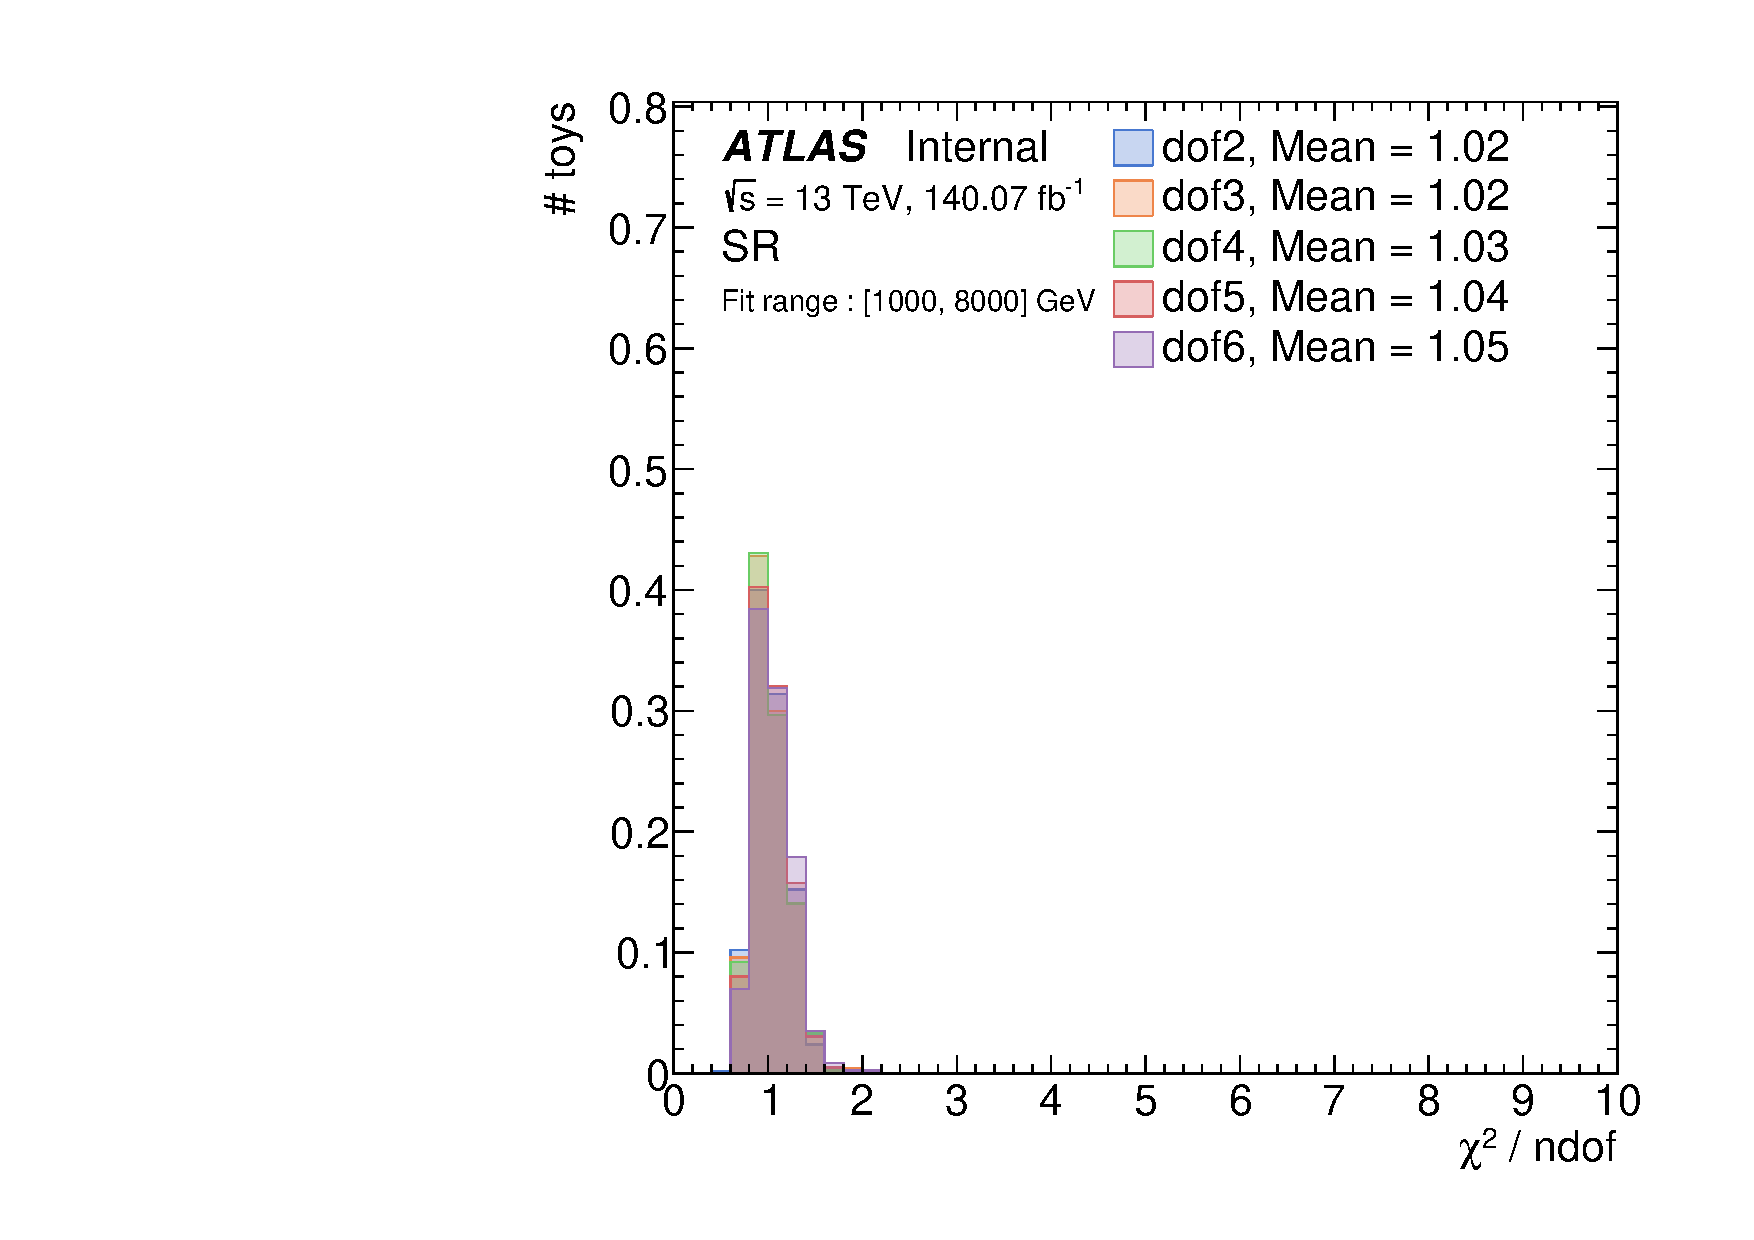
\includegraphics[width=0.8\textwidth]{5_resonances/bkg/modeling/ftest/SR/can__photonjet_Pythia_jfakeisosmooth__SR__chi2ndof__range_1000_8000__toys}
        \caption{SR}
    \end{subfigure}
    \begin{subfigure}[h]{0.49\linewidth}
        \centering
        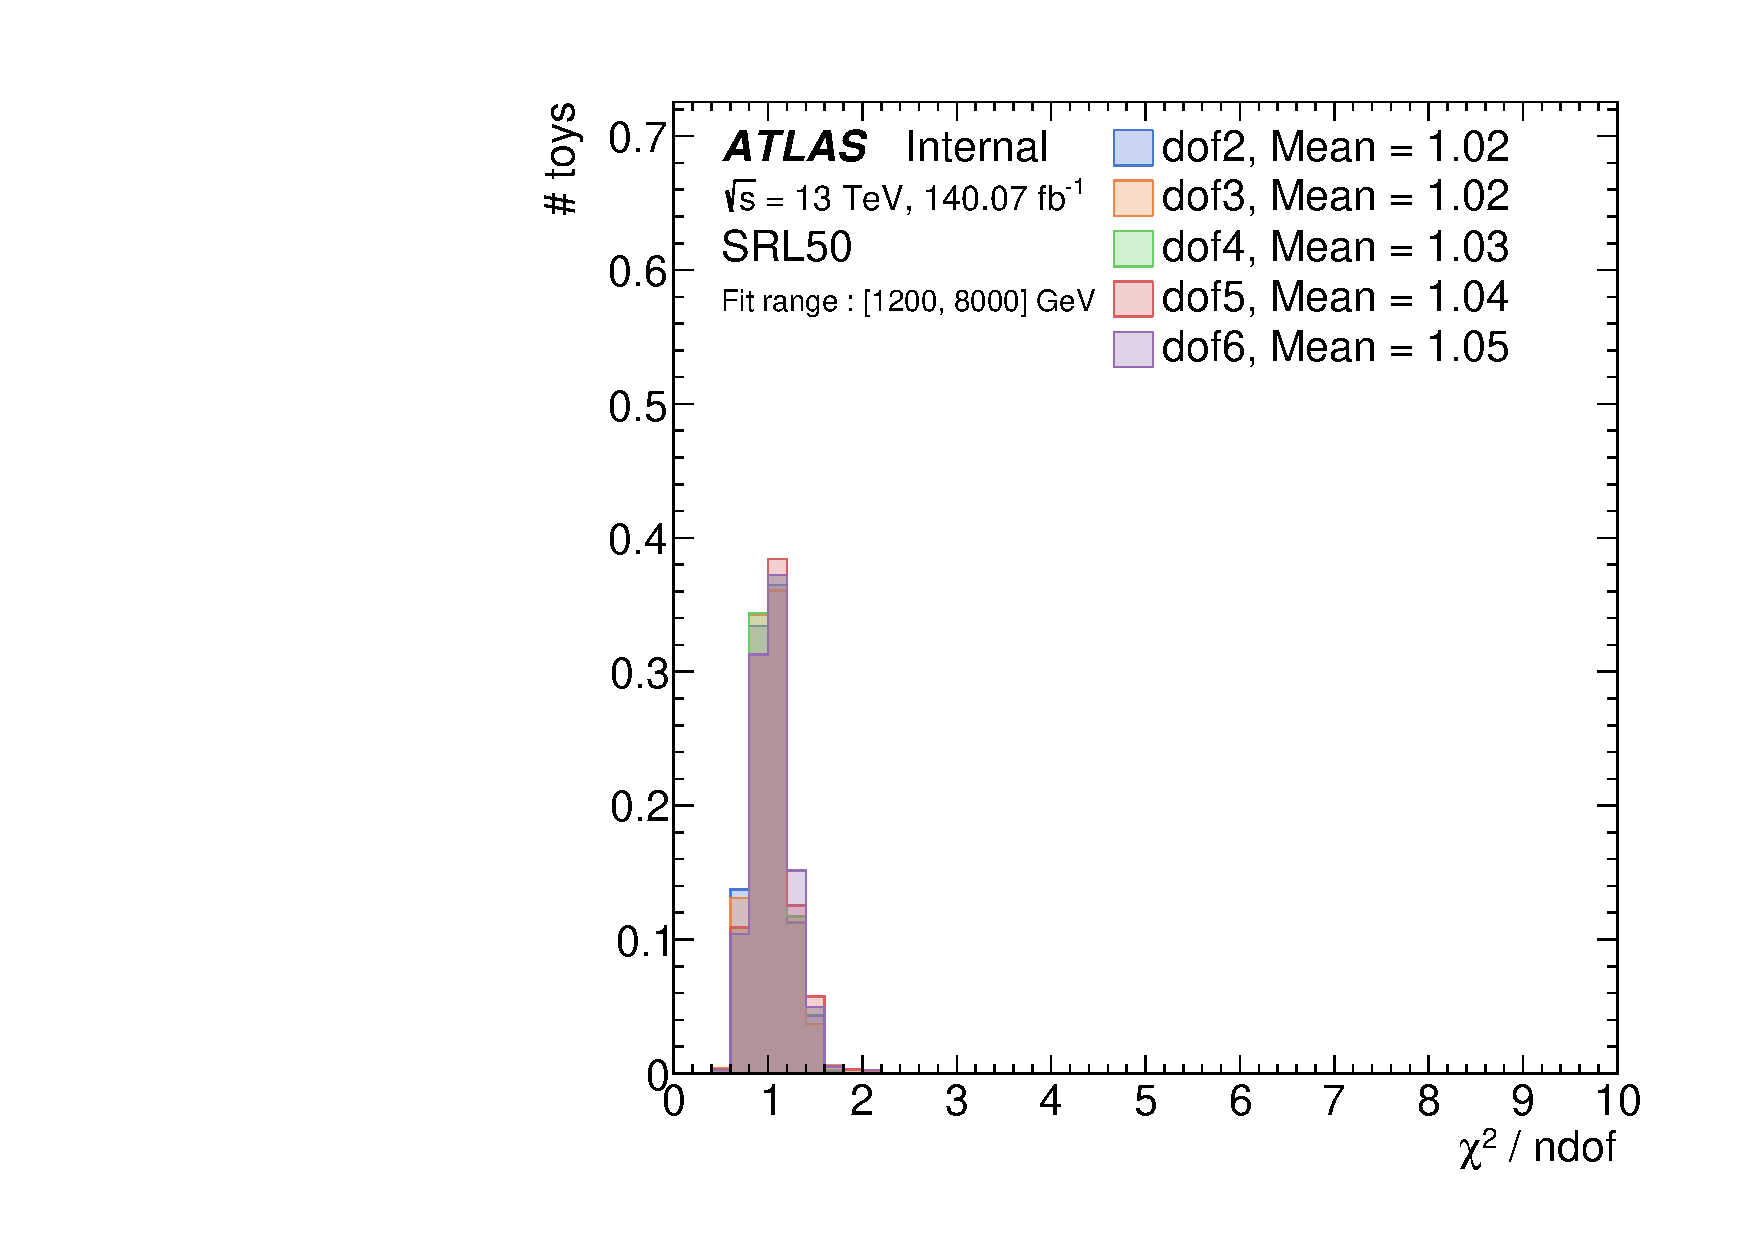
\includegraphics[width=0.8\textwidth]{5_resonances/bkg/modeling/ftest/SRL50/can__photonjet_Pythia_jfakeisosmooth__SRL50__chi2ndof__range_1200_8000__toys}
        \caption{SRL}
    \end{subfigure}
    \\
    \begin{subfigure}[h]{0.49\linewidth}
        \centering
        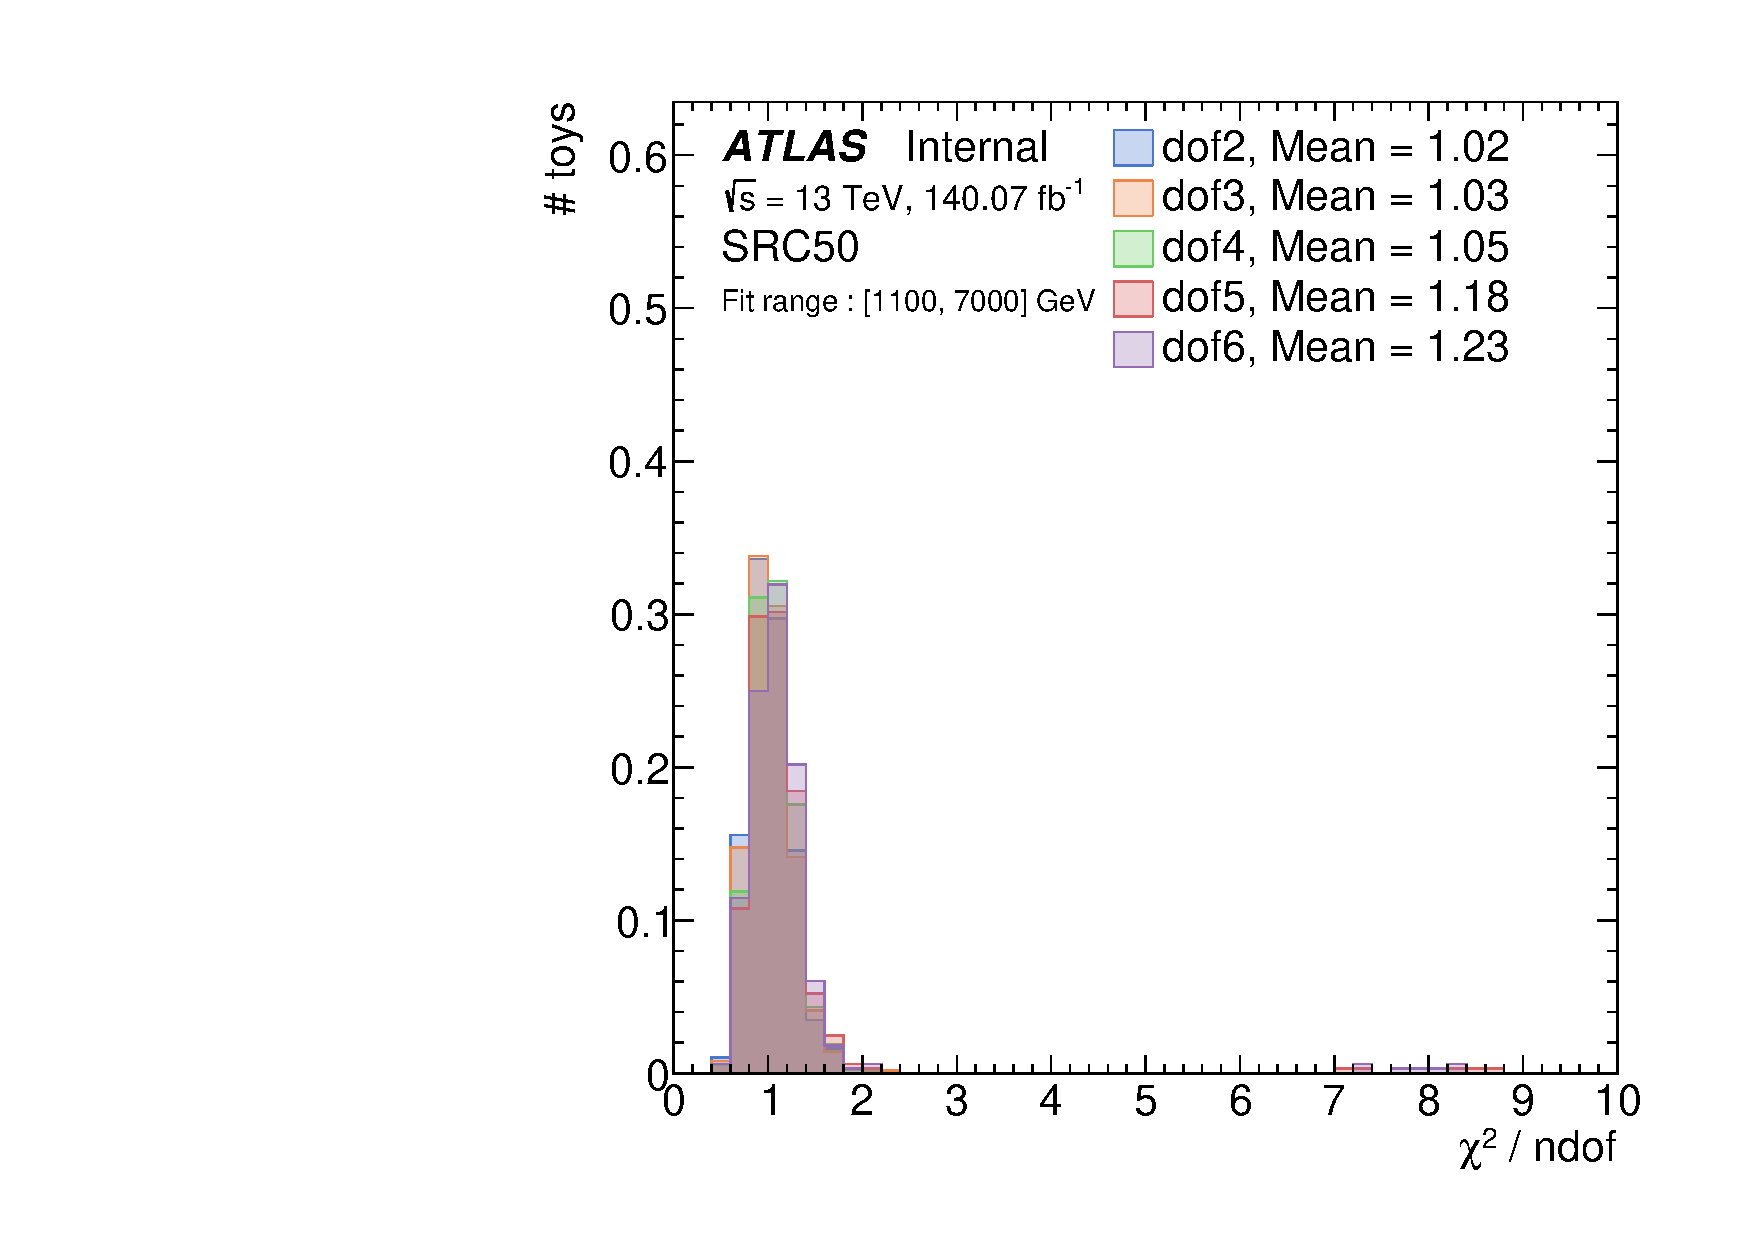
\includegraphics[width=0.8\textwidth]{5_resonances/bkg/modeling/ftest/SRC50/can__photonjet_Pythia_jfakeisosmooth__SRC50__chi2ndof__range_1100_7000__toys}
        \caption{SRC}
    \end{subfigure}
    \begin{subfigure}[h]{0.49\linewidth}
        \centering
        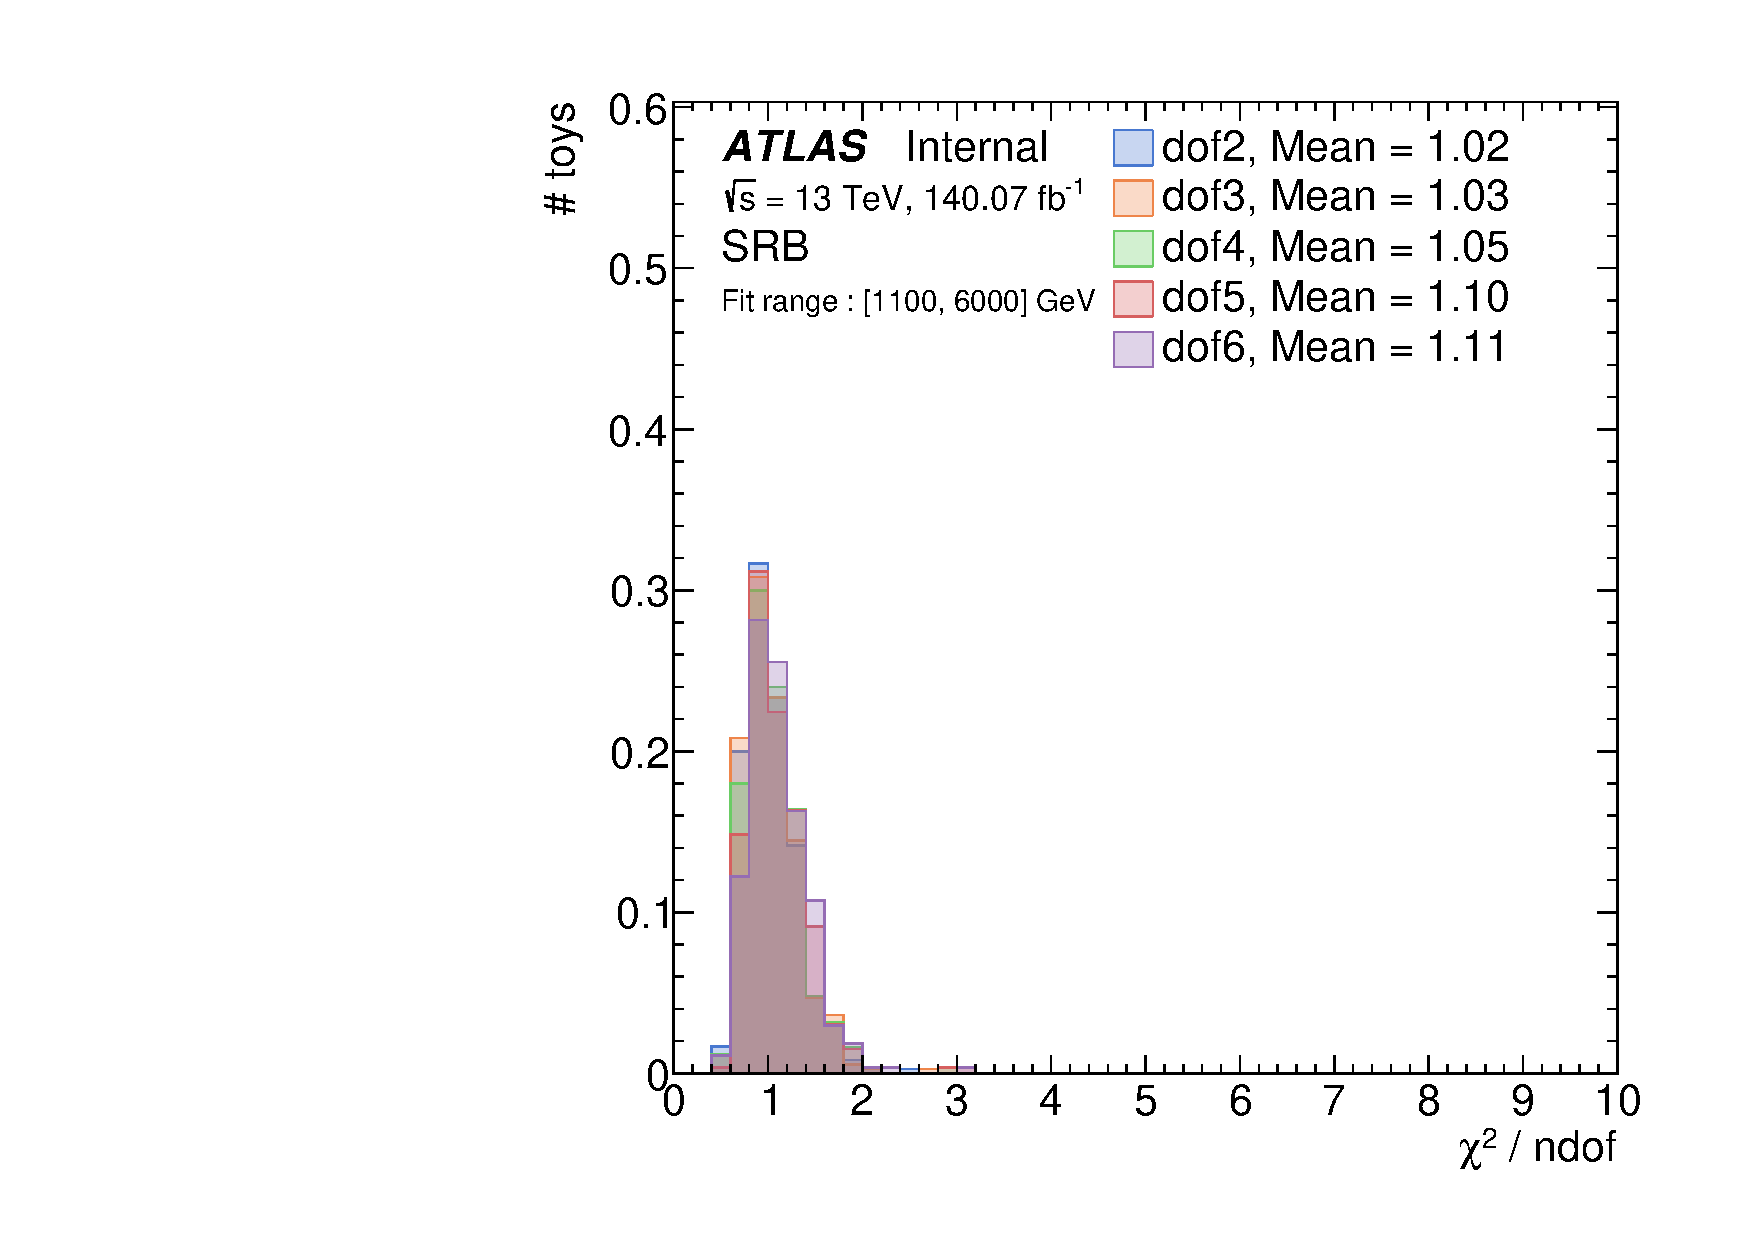
\includegraphics[width=0.8\textwidth]{5_resonances/bkg/modeling/ftest/SRB/can__photonjet_Pythia_jfakeisosmooth__SRB__chi2ndof__range_1100_6000__toys}
        \caption{SRB}
    \end{subfigure}
    \caption{Distribución de \(\chisq / \text{ndof}\) para cada modelo funcional en cada región de se\~nal.}
    \label{fig:bkg:modeling:preparation:ftest:chi2ndof}
\end{figure}

\begin{figure}[ht!]
    \centering
    \begin{subfigure}[h]{0.49\linewidth}
        \centering
        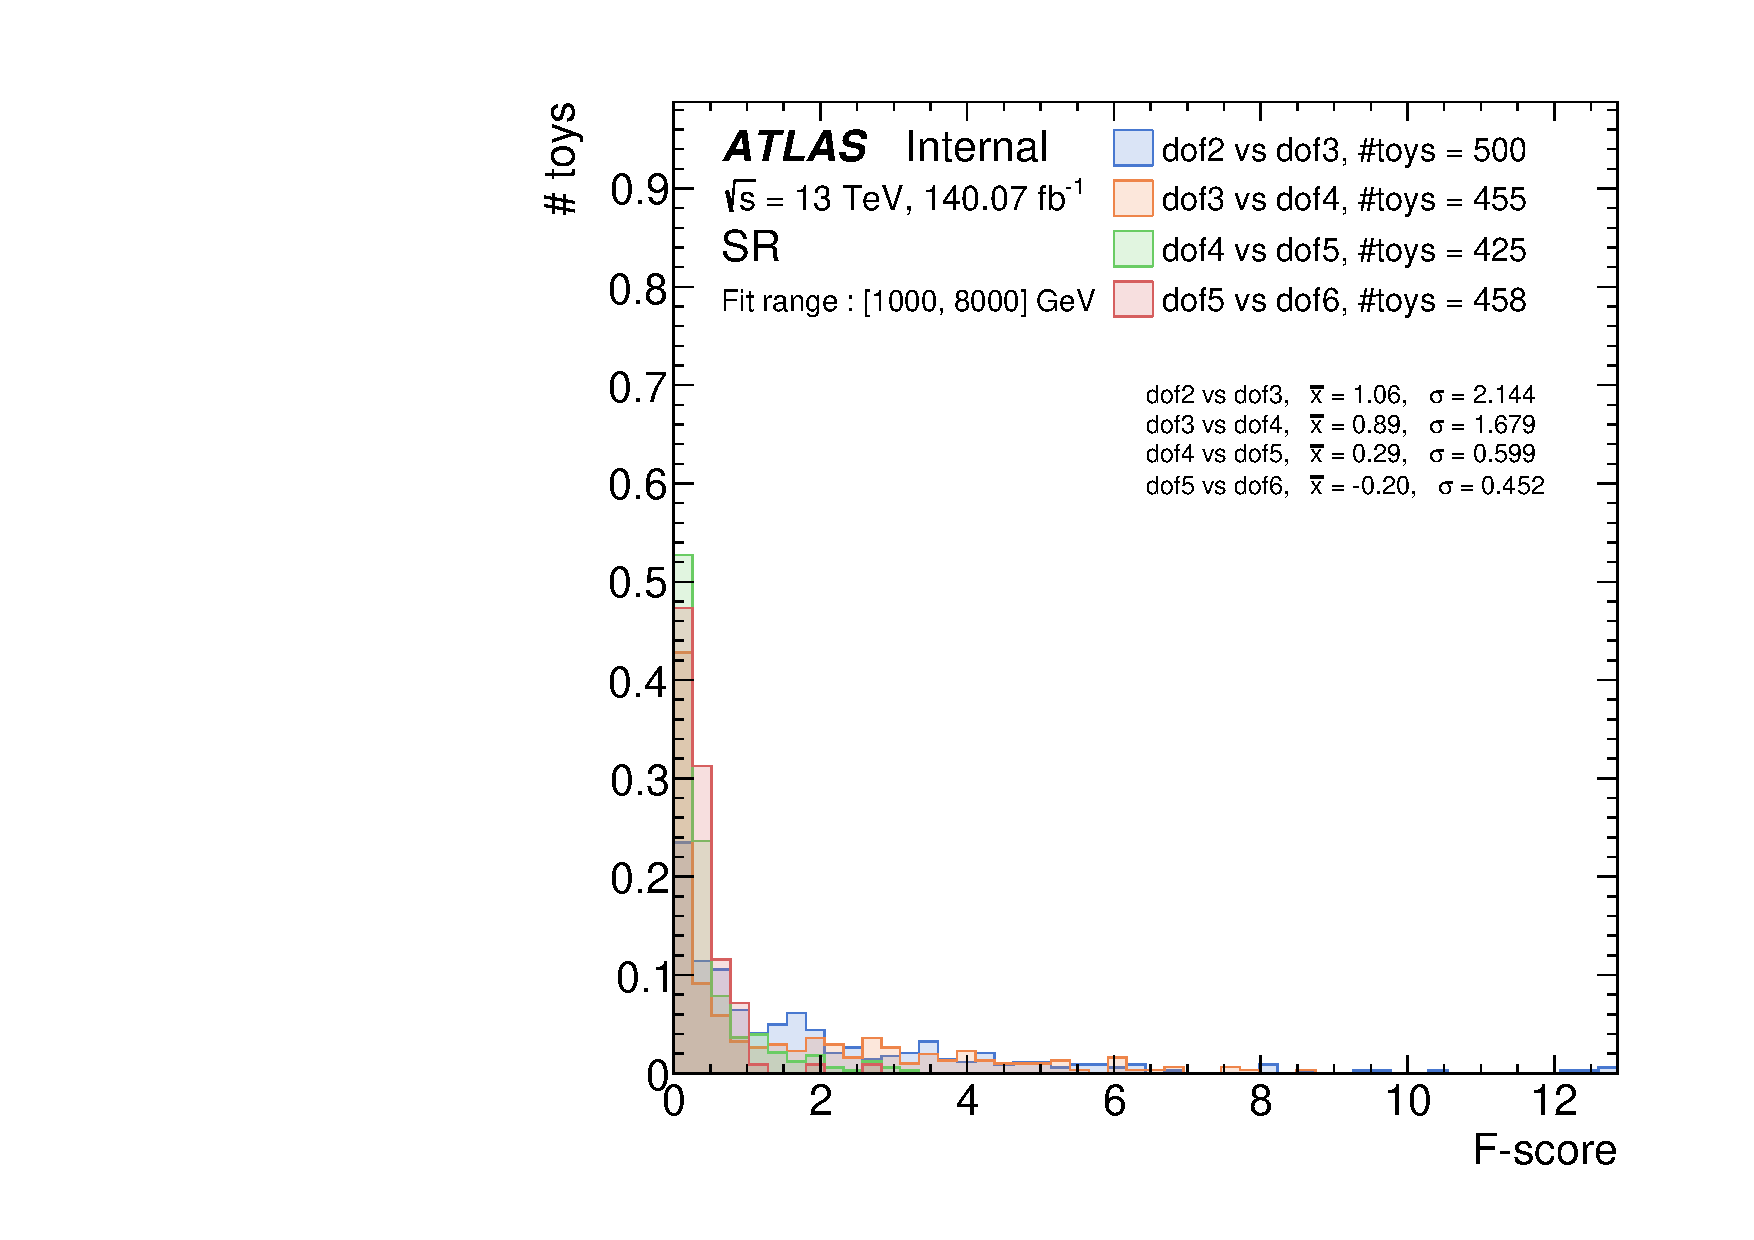
\includegraphics[width=0.8\textwidth]{5_resonances/bkg/modeling/ftest/SR/can__photonjet_Pythia_jfakeisosmooth__SR__fvalue__range_1000_8000__toys}
        \caption{SR}
    \end{subfigure}
    \begin{subfigure}[h]{0.49\linewidth}
        \centering
        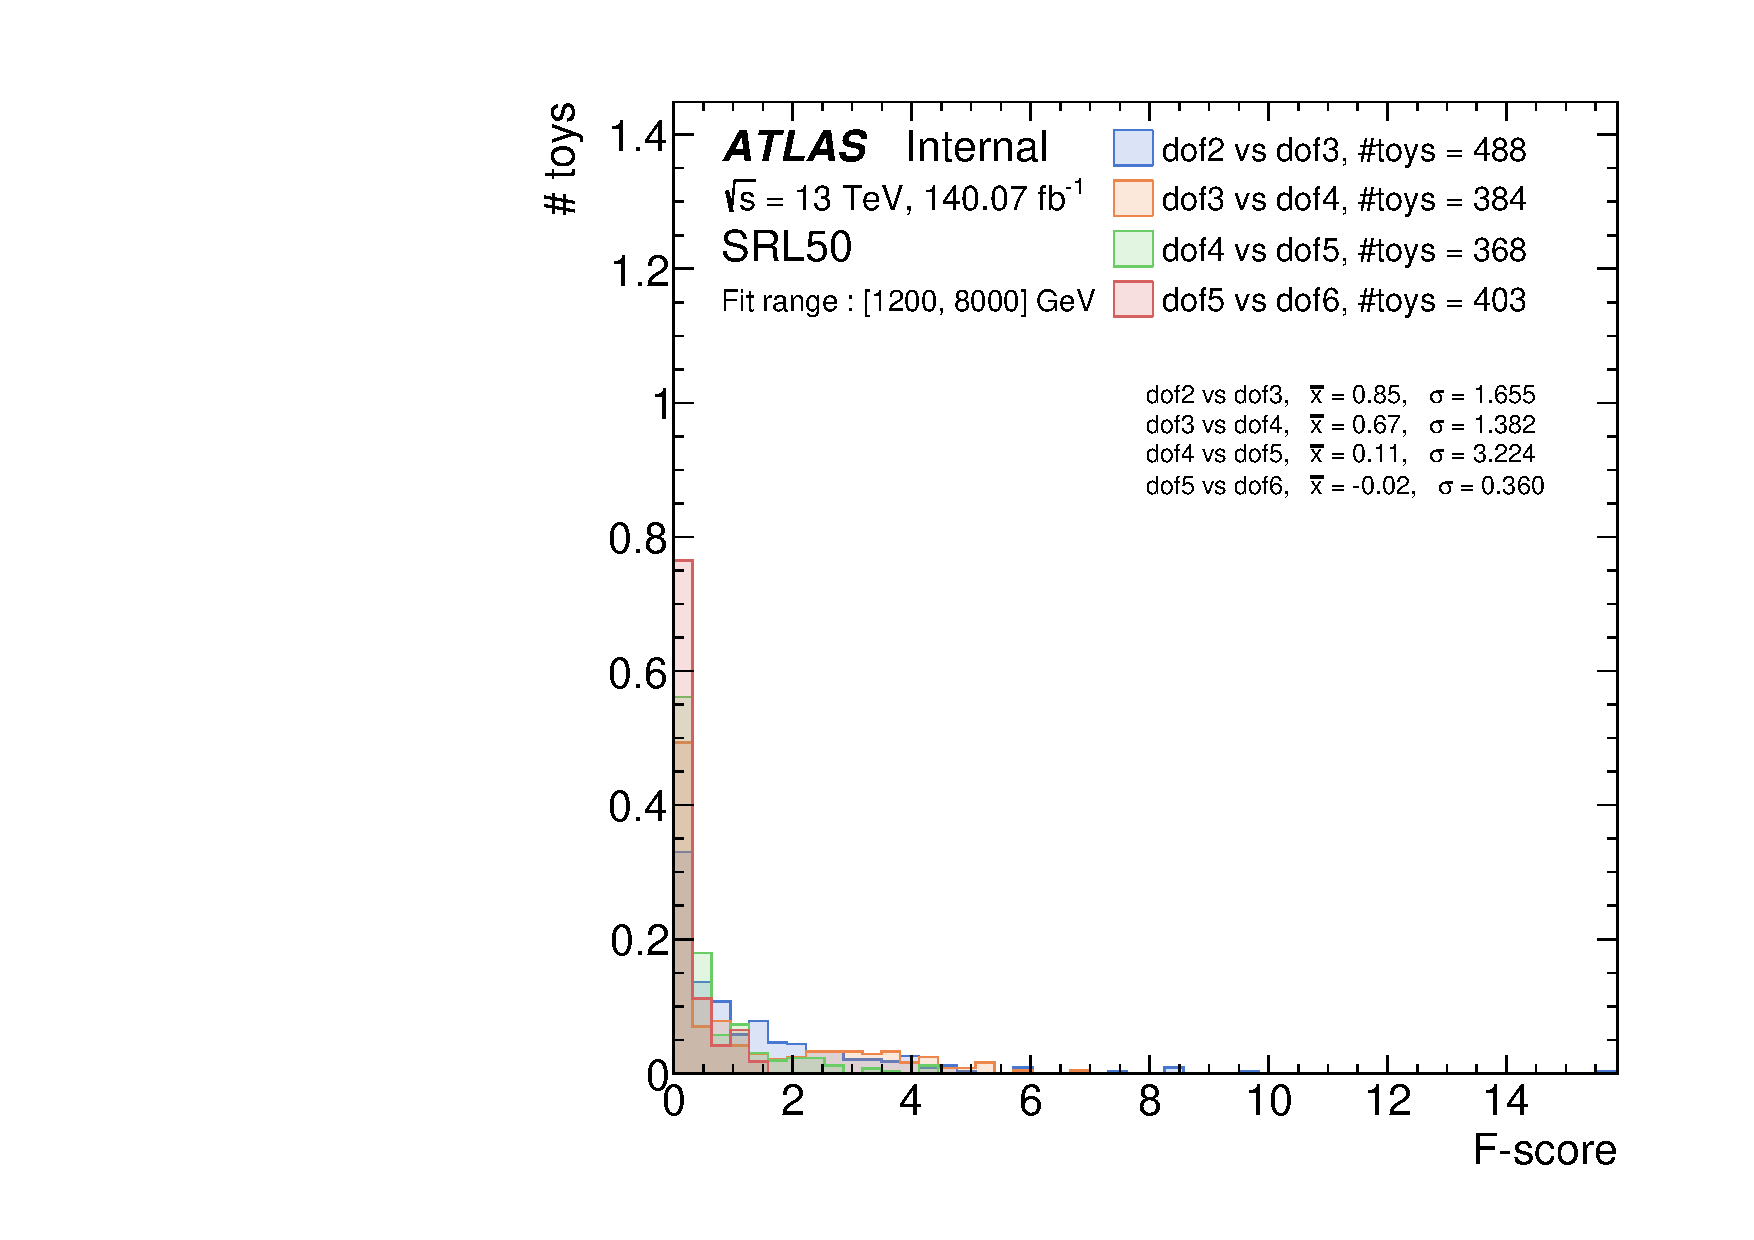
\includegraphics[width=0.8\textwidth]{5_resonances/bkg/modeling/ftest/SRL50/can__photonjet_Pythia_jfakeisosmooth__SRL50__fvalue__range_1200_8000__toys}
        \caption{SRL}
    \end{subfigure}
    \\
    \begin{subfigure}[h]{0.49\linewidth}
        \centering
        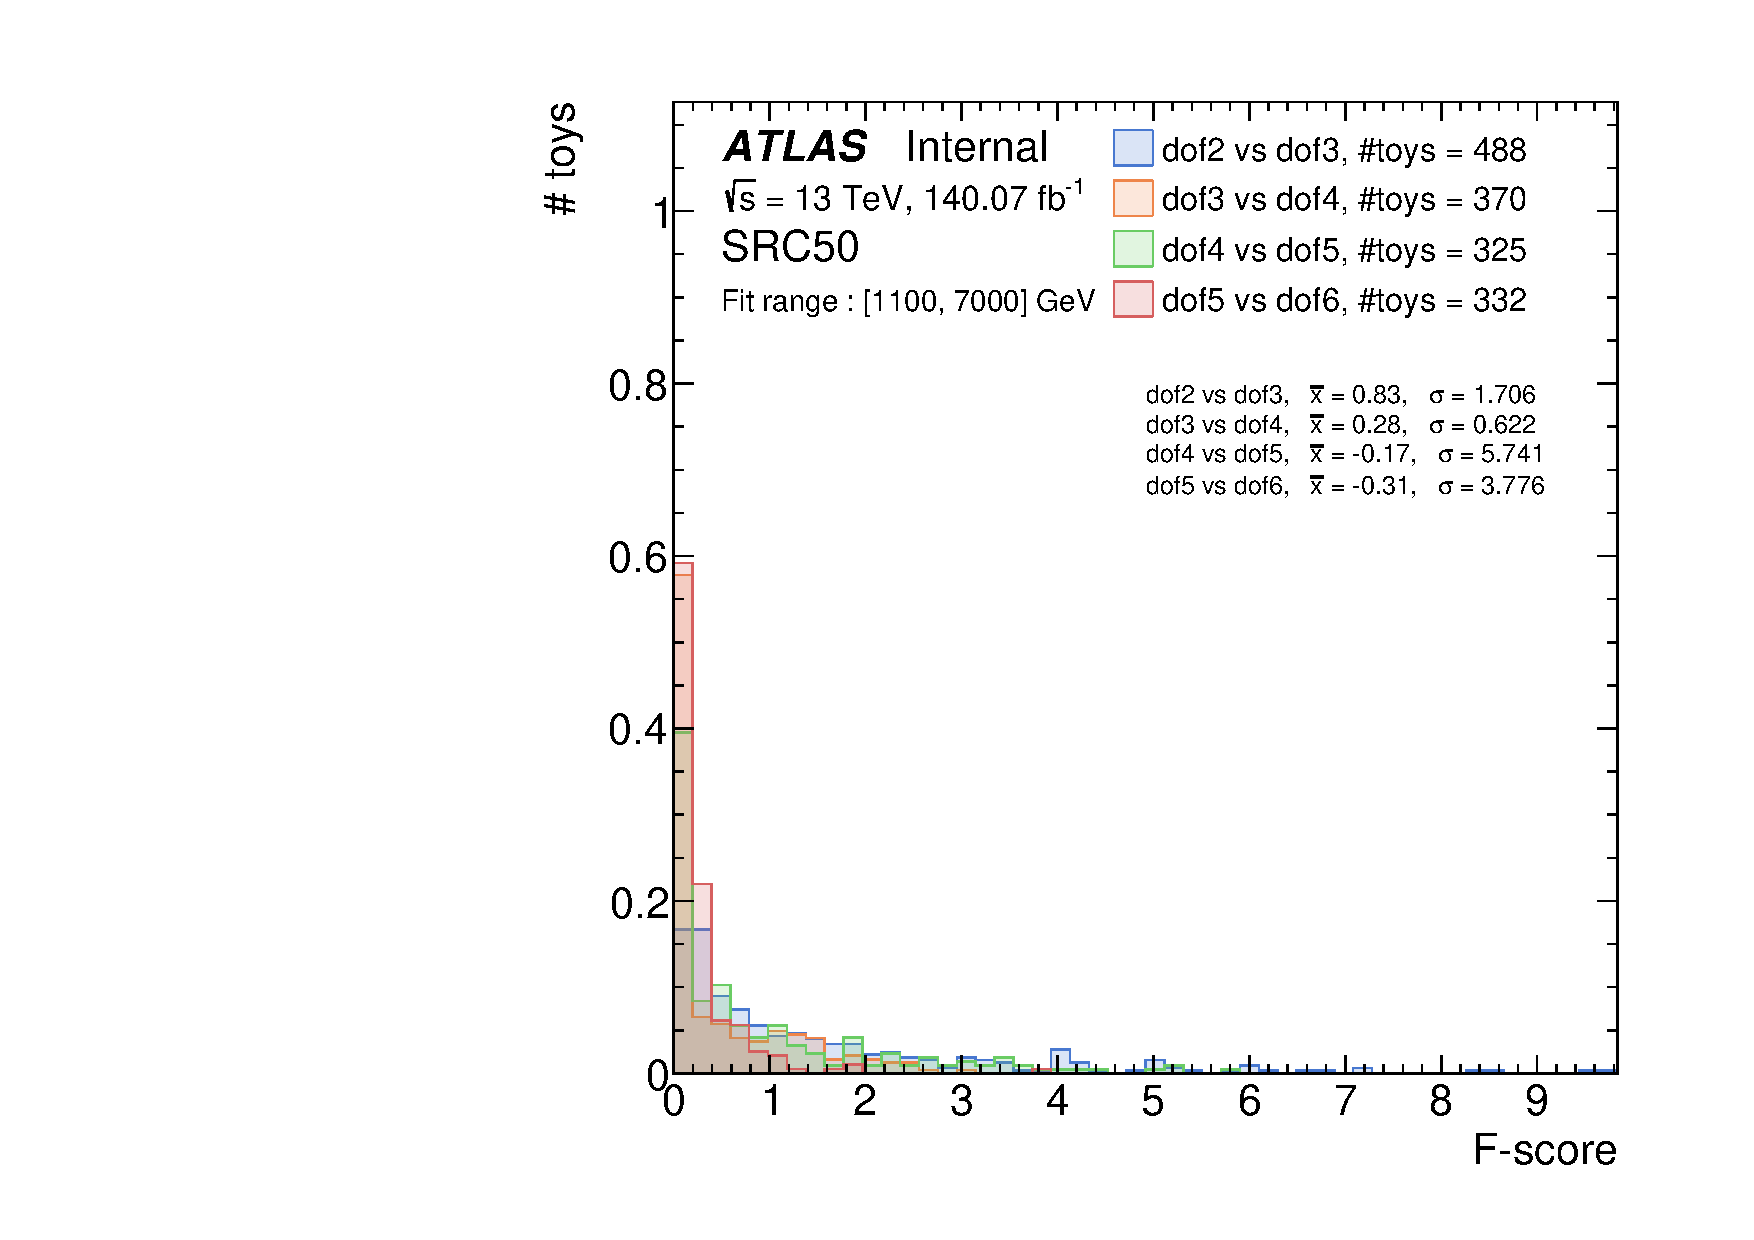
\includegraphics[width=0.8\textwidth]{5_resonances/bkg/modeling/ftest/SRC50/can__photonjet_Pythia_jfakeisosmooth__SRC50__fvalue__range_1100_7000__toys}
        \caption{SRC}
    \end{subfigure}
    \begin{subfigure}[h]{0.49\linewidth}
        \centering
        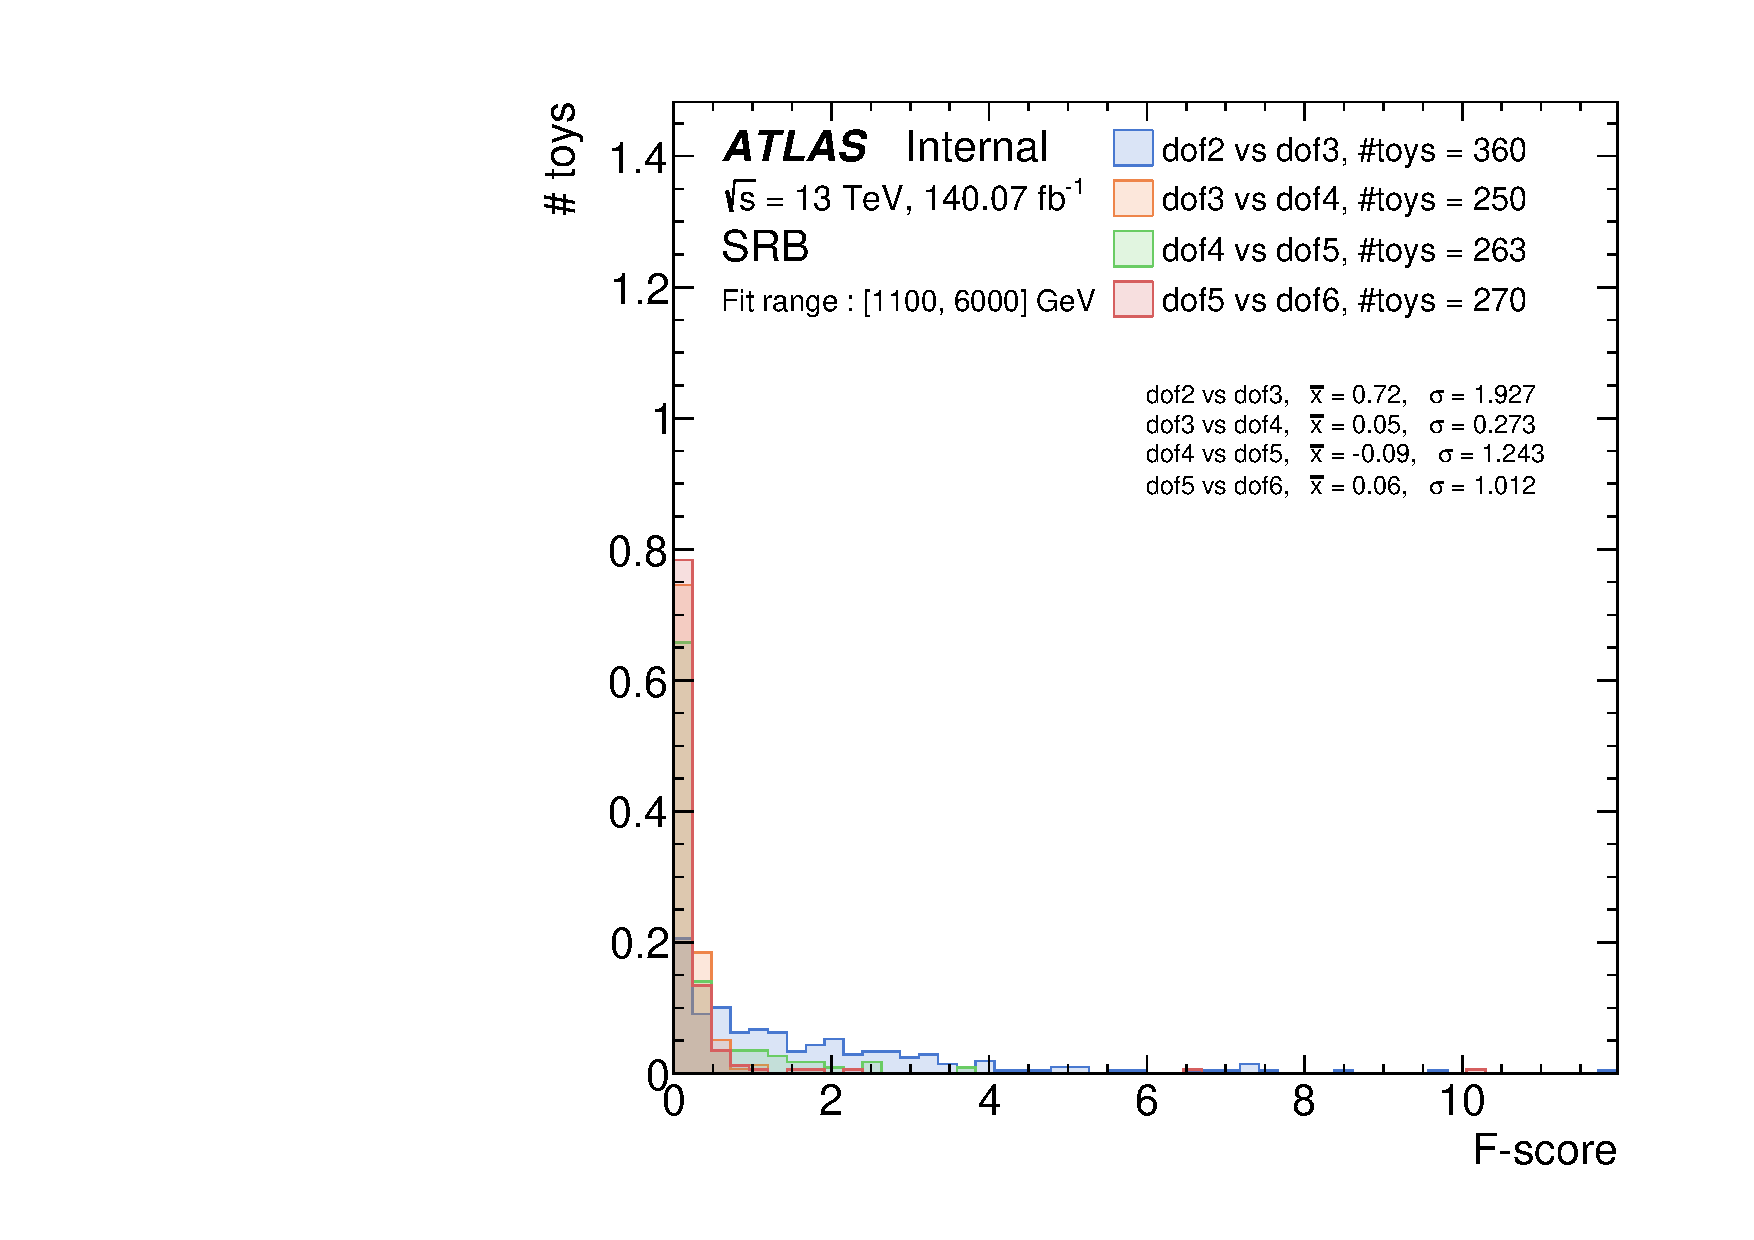
\includegraphics[width=0.8\textwidth]{5_resonances/bkg/modeling/ftest/SRB/can__photonjet_Pythia_jfakeisosmooth__SRB__fvalue__range_1100_6000__toys}
        \caption{SRB}
    \end{subfigure}
    \caption{Distribuciones del estadístico \(F\). Los tests se realizan comparando dos modelos funcionales a la misma vez, mostrado por cada histograma. Para cada uno de ellos, se indica el número de toys con el que fue realizado, así como también le valor medio de la distribución (\(\bar{x}\)) y el ancho (\(\sigma\)).}
    \label{fig:bkg:modeling:preparation:ftest:ftest}
\end{figure}

\begin{figure}[ht!]
    \centering
    \begin{subfigure}[h]{0.49\linewidth}
        \centering
        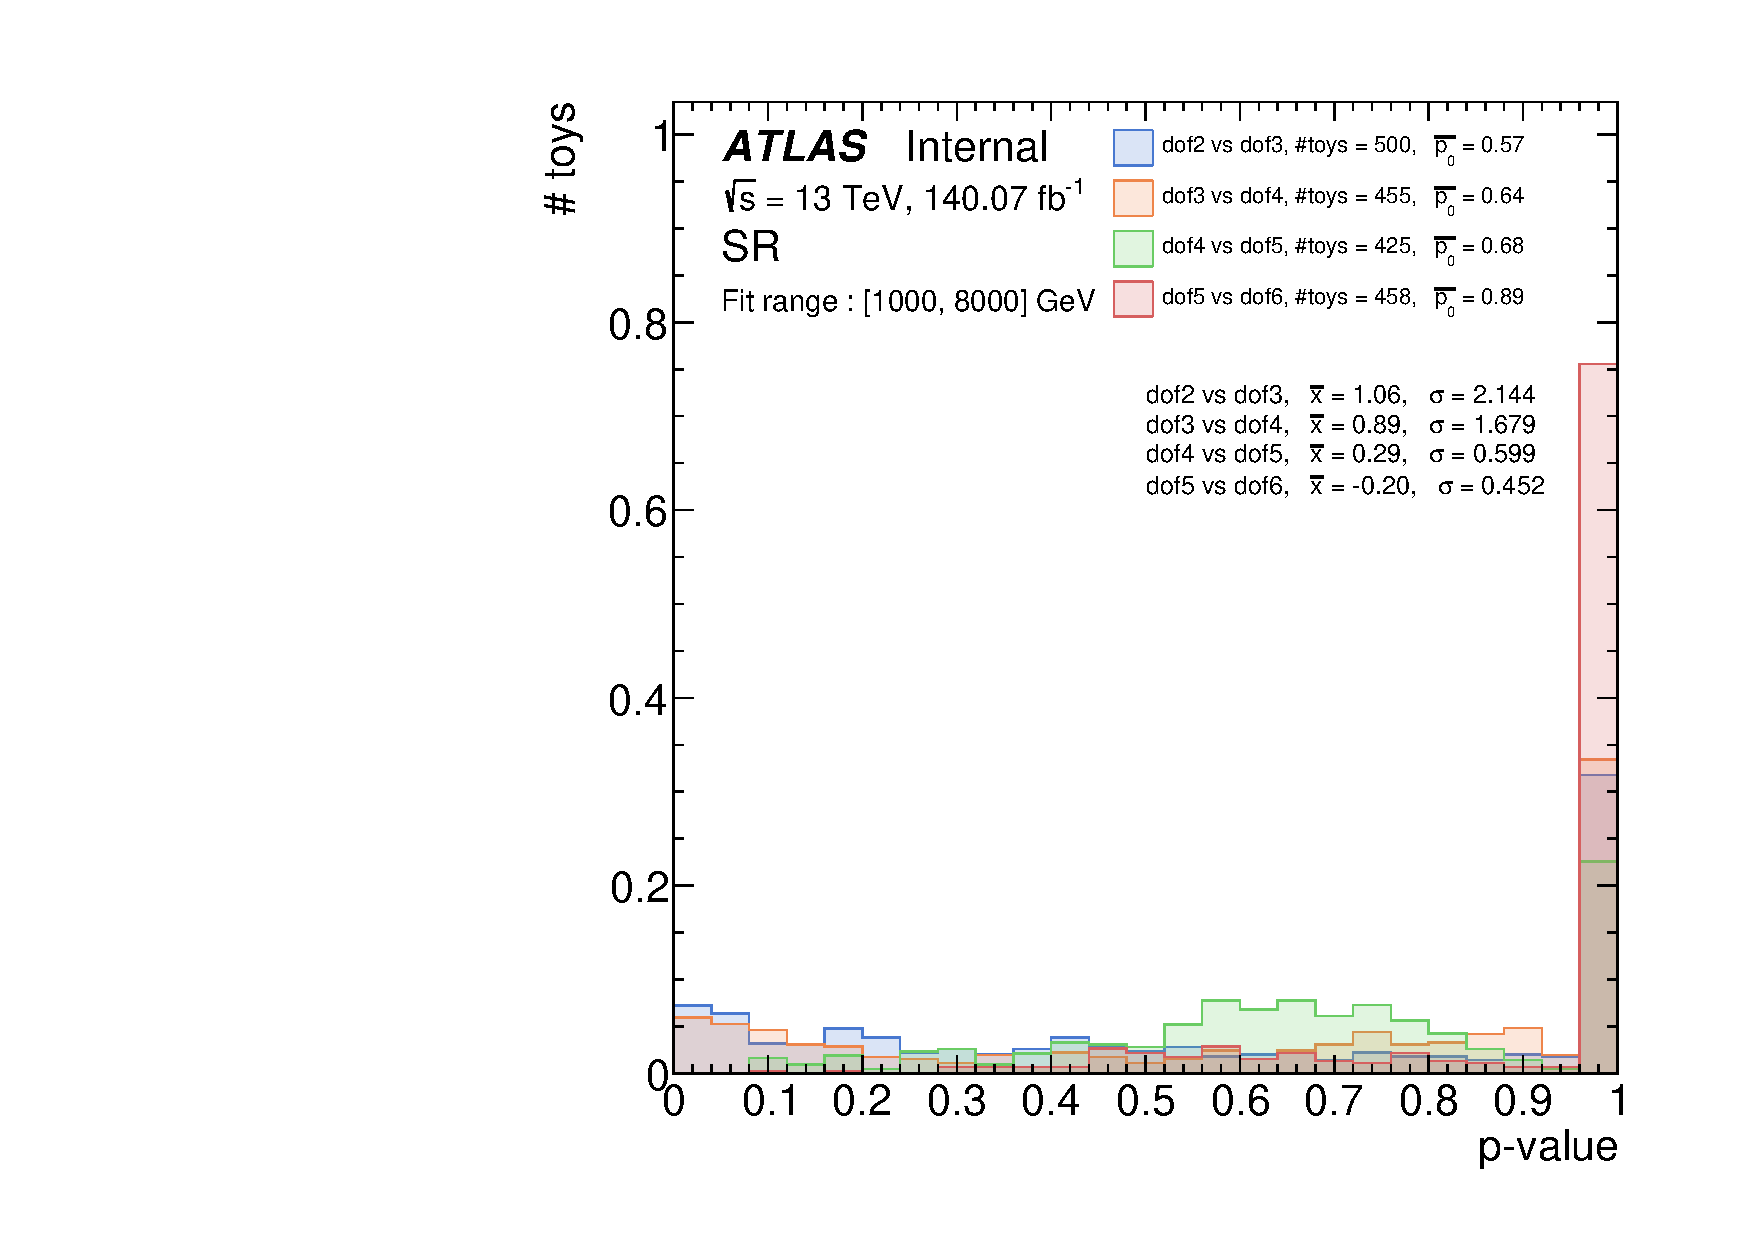
\includegraphics[width=0.8\textwidth]{5_resonances/bkg/modeling/ftest/SR/can__photonjet_Pythia_jfakeisosmooth__SR__fvalue_pvalue__range_1000_8000__toys}
        \caption{SR}
    \end{subfigure}
    \begin{subfigure}[h]{0.49\linewidth}
        \centering
        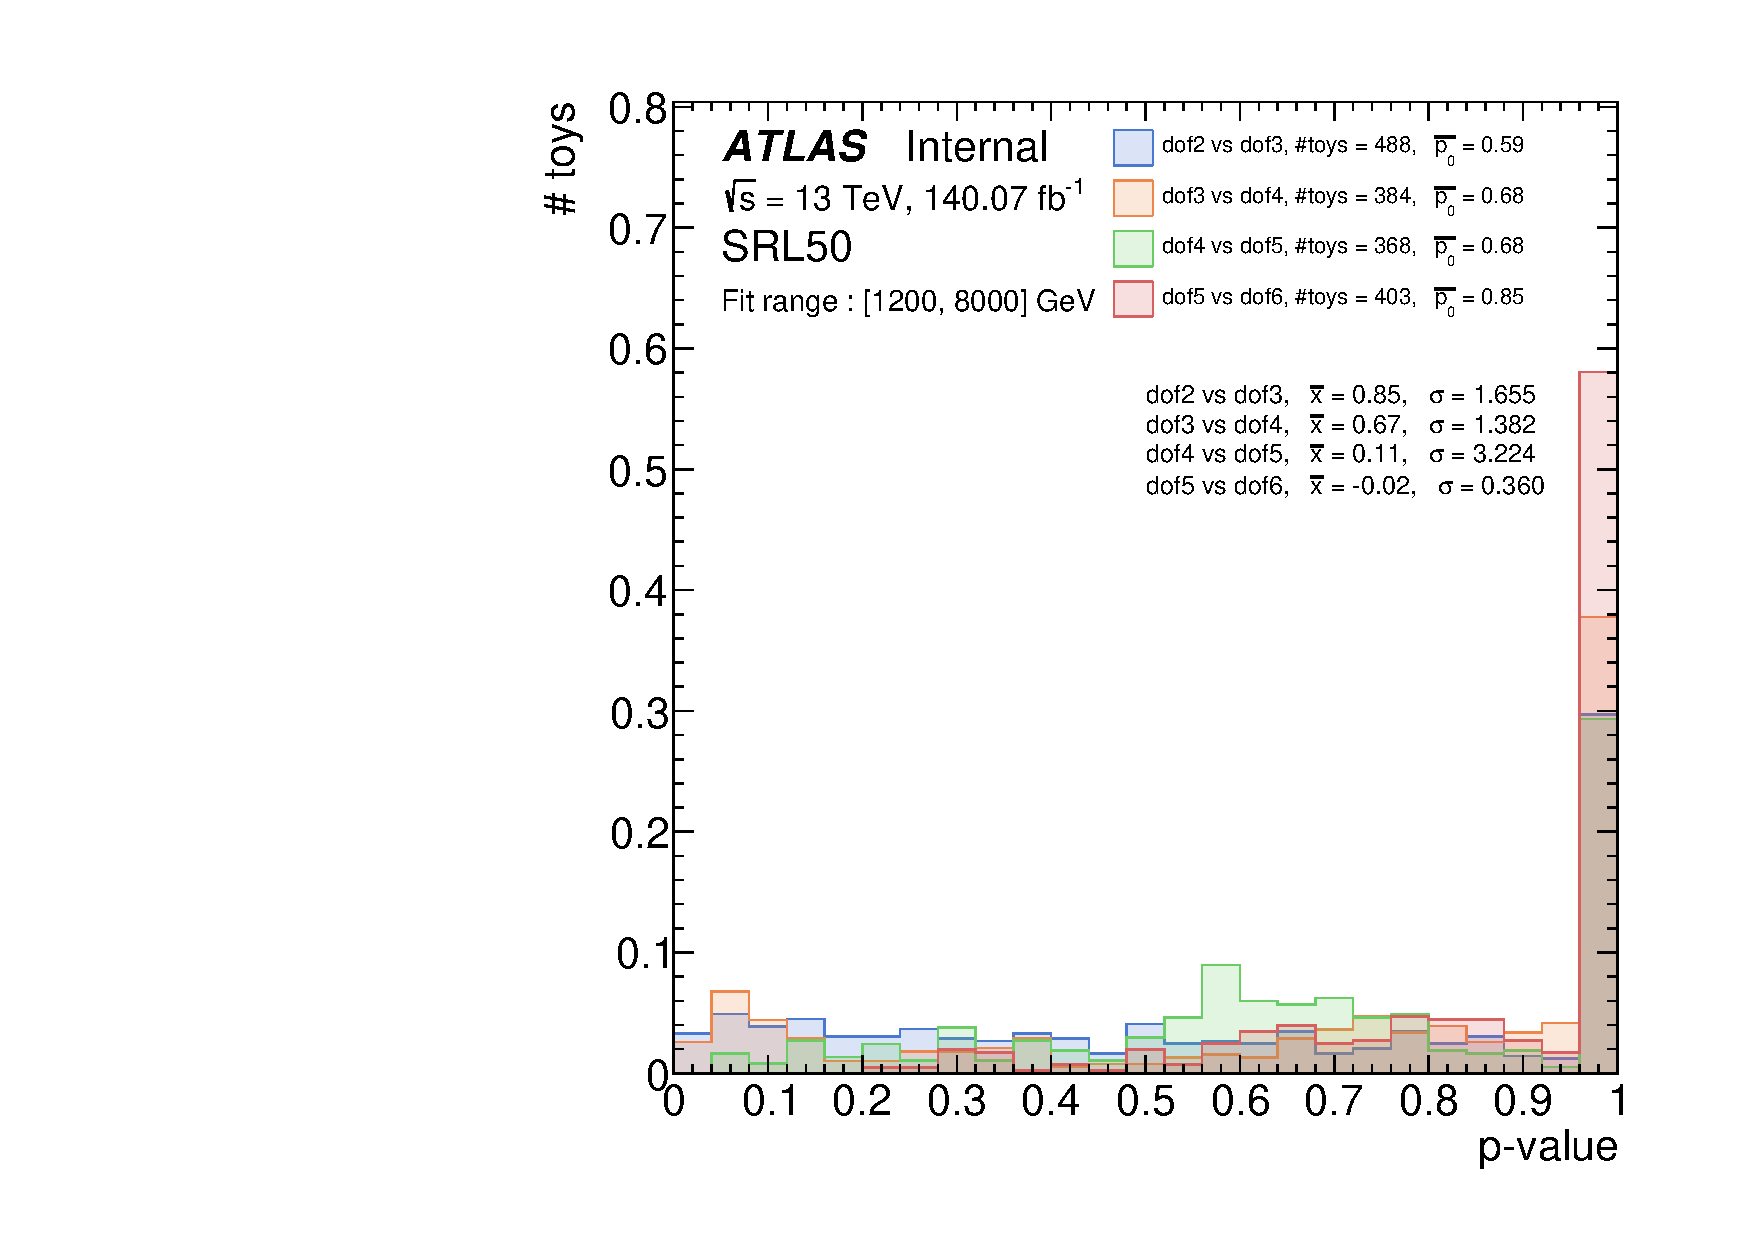
\includegraphics[width=0.8\textwidth]{5_resonances/bkg/modeling/ftest/SRL50/can__photonjet_Pythia_jfakeisosmooth__SRL50__fvalue_pvalue__range_1200_8000__toys}
        \caption{SRL}
    \end{subfigure}
    \\
    \begin{subfigure}[h]{0.49\linewidth}
        \centering
        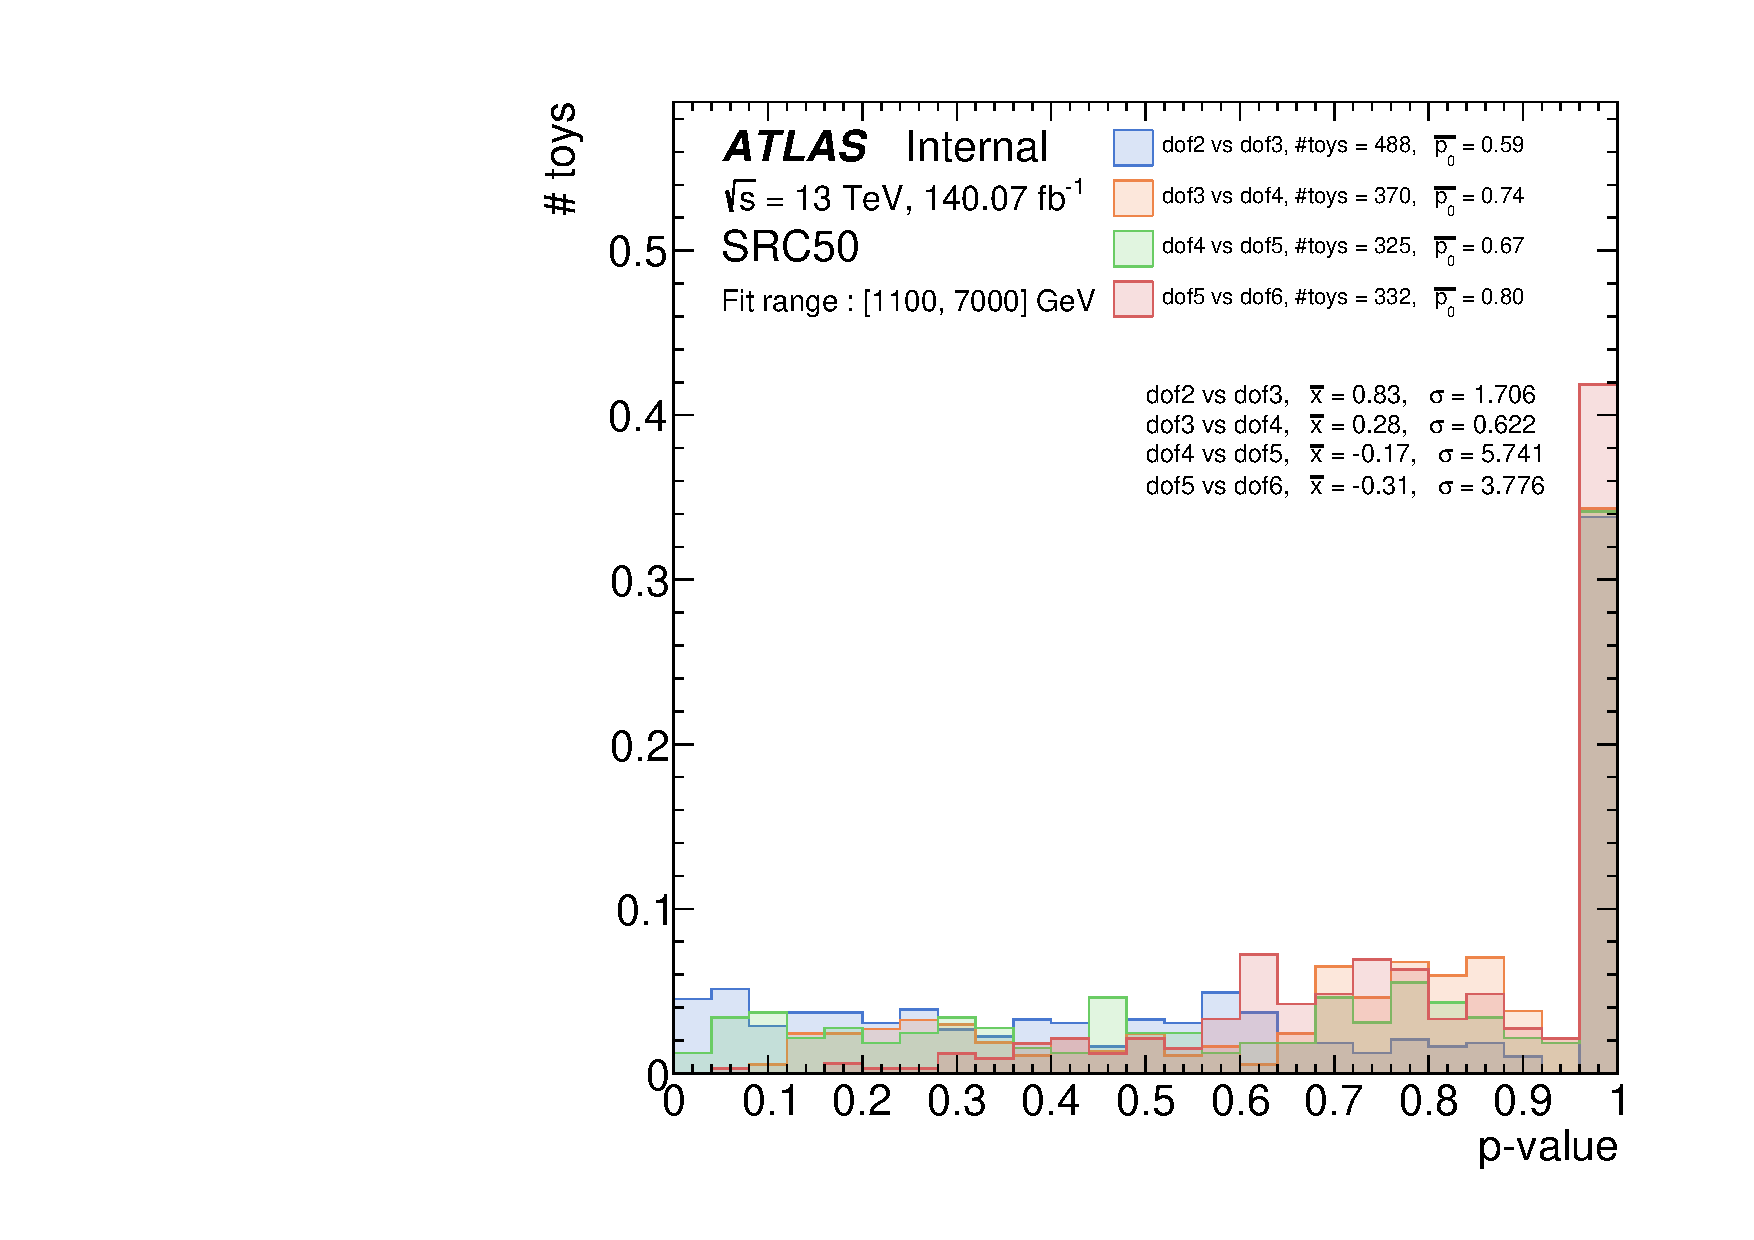
\includegraphics[width=0.8\textwidth]{5_resonances/bkg/modeling/ftest/SRC50/can__photonjet_Pythia_jfakeisosmooth__SRC50__fvalue_pvalue__range_1100_7000__toys}
        \caption{SRC}
    \end{subfigure}
    \begin{subfigure}[h]{0.49\linewidth}
        \centering
        \includegraphics[width=0.8\textwidth]{5_resonances/bkg/modeling/ftest/SRB/can__photonjet_Pythia_jfakeisosmooth__SRB__fvalue_pvalue__range_1100_6000__toys}
        \caption{SRB}
    \end{subfigure}
    \caption{Distribución de los valores \(p\) del estadítico \(F\), comparando el rendimiento de cada par de funciones. Los valores medios y anchos mostrados corresponden a los de la distribución del estadístico \(F\), mientras que el valor \(p\) promedio se se\~nala en cada caso.}
    \label{fig:bkg:modeling:preparation:ftest:ftest_pvalue}
\end{figure}

La \Fig{\ref{fig:bkg:modeling:preparation:ftest:chi2ndof}} muestra las distribuciones \(\chisq / \text{ndof}\) de cada uno de los modelos para diferentes regiones de señal calculadas a partir de toys. Se puede observar que todas las distribuciones están centradas en \(\sim 1\), lo que significa que en general todos los modelos describen correctamente la distribución de \ac{BO}. Para cuantificar el comportamiento de los diferentes modelos entre ellos, las distribuciones del valor \(F\) se muestran en la \Fig{\ref{fig:bkg:modeling:preparation:ftest:ftest}} en las diferentes regiones de señal, comparando dos modelos a la vez. Para cada par, se muestra el número de toys que convergen para ambos modelos, así como el valor medio y los anchos de las distribuciones. Asimismo, en la \Fig{\ref{fig:bkg:modeling:preparation:ftest:ftest_pvalue}} se puede observar la distribución de valores \(p\) para el test \(F\), que muestra que todas las comparaciones entre modelos conducen a valores \(p(F)\) muy cercanos a 1 indicando que ningún modelo se ajusta mejor que otro a las distribuciones. Por esta razón, no se descarta ningún modelo funcional utilizando el test \(F\).





































\subsection{Resumen de las estrategias del modelado del fondo}
\label{subsec:bkg:modeling:strategy_summary}

A lo largo de esta sección se han realizado diferentes tests estadísticos para determinar la óptima combinación de rango y función de ajuste para modelar la distribución de fondo en los datos. Estos tests se han realizado para cada una de las regiones de señal consideradas en el análisis, y también para cada modelo de señal.

En el primer paso, se realizaron tests de \ac{SSig} para decidir cuáles de estas combinaciones de rangos y funciones minimizan la aparición de cualquier señal al realizar los ajustes de \ac{BO}. Además, la incerteza de modelado de fondo resulta de esta prueba, lo que significa que el uso de la combinación que conduzca a la menor \ac{SSig}, también influirá en las incertezas finales al realizar la búsqueda en los datos. Para cada rango de ajuste, se clasifican los modelos funcionales y se pasan todos por los tests de \ac{SI} y tests \(F\). La primera comprueba si la función es capaz de capturar toda la señal inyectada al fondo, y la segunda comprueba si añadiendo otro \ac{dof} a la función se observa una mejora significativa en los ajustes.

Como se discute en la \Sect{\ref{sec:strategy:stat_treatment:fits_results}}, se estudian dos tipos de ajustes a los datos. En los ajustes de \ac{BO}, sólo se tiene en cuenta la forma funcional del fondo y la intensidad de la señal en la \Eqn{\ref{eq:strategy:stat_treatment:stat_model:likelihood}} se fija en 0. Estos ajustes se realizan en las regiones SR, SRB y SRC, utilizando las funciones y rangos indicados en la \Tab{\ref{tab:bkg:modeling:strategy_modeling:summary}}.
Por otro lado, para la interpretación de \ac{SB} se deja variar la intensidad de la señal \(\mu\) y se cuantifica la señal resultante del ajuste. Los ajustes a los datos se realizan entonces con un modelo \ac{SB}, en el que el componente de señal es una \ac{PDF2} y la función de fondo difiere para cada modelo y región de señal.

En la \Tab{\ref{tab:bkg:modeling:strategy_modeling:summary}}, se muestra un resumen de las formas funcionales y los rangos de ajuste para cada modelo y región de señal. Para los ajustes de \ac{BO}, se eligen utilizar las funciones y rangos óptimos que se encontraron para los modelos de \qstar, \bstar y \cstar, ya que ellos arrojan los menores valores de \ac{SSig}. 
Los modelos de \ac{QBH} son estudiados sólo en la región inclusiva, ya que se espera que esté dominado mayormente por jets lights, teniendo entonces muy bajas eficiencias de selección de \bjets y \cjets.
Para realizar interpretaciones sobre el modelo de \qstar, se considera la región inclusiva SR. En esta región es donde se observa la mayor significancia (ver la \Tab{\ref{tab:signals:acc_eff:qstar_signficances}}), y se encontró que hacer fits simultáneos en las 3 regiones ortogonales no brindaba ningún beneficio significativo. De forma similar para los \bstar en la región SRB, se encuentra aquí la mayor significancia de esta se\~nal, es por ello que se decide utilizar sólo la región SRB. Finalmente, como se discutió en la \Sect{\ref{sec:signals:acc_eff}}, una gran mejora en las significancias puede lograrse al realizar los estudios con las se\~nales de \cstar en las 3 regiones SRL, SRB y SRC en simultáneo.


\begin{table}[ht!]
    \centering
    \caption{Resumen de los rangos (en GeV) y las funciones que son ajustadas a los datos para cada región del análisis y modelo de se\~nal. La última columna indica si un ajuste simultáneo es realizado utilizando las regiones SRB, SRL y SRC.}
    \resizebox{\linewidth}{!}{
        \begin{tabular}{lccccc}
            \toprule
                                & SR                      & SRL                               & SRC                               & SRB                               & \begin{tabular}{@{}c@{}} Ajuste simultáneo \\SRC+SRB+SRL? \end{tabular}\\
            \midrule
            \ac{BO}             & \textit{dof2}, \([1000,8000]\)    & \textit{dof2}, \([1200,8000]\)    & \textit{dof4}, \([1100,7000]\)    & \textit{dof2}, \([1100,6000]\)    & No                      \\
            \midrule
            Gaussianas          & \textit{dof3}, \([1200,8000]\)    & \textit{dof3}, \([1500,8000]\)    & \textit{dof4}, \([1000,7000]\)    & \textit{dof5}, \([900,7000]\)     & No                      \\
            \ac{QBH}            & \textit{dof5}, \([1000,8000]\)    & -                                 & -                                 & -                                 & -                       \\
            \ac{EQ}, \qstar     & \textit{dof2}, \([1000,8000]\)    & -                                 & -                                 & -                                 & -                       \\
            \ac{EQ}, \cstar     & -                                 & \textit{dof2}, \([1200,8000]\)    & \textit{dof4}, \([1100,7000]\)    & \textit{dof2}, \([1100,6000]\)    & Yes                     \\
            \ac{EQ}, \bstar     & -                                 & -                                 & -                                 & \textit{dof2}, \([1100,6000]\)    & -                       \\
            \bottomrule
        \end{tabular}
    }
    \label{tab:bkg:modeling:strategy_modeling:summary}
\end{table}

